% The class: the leet one
\documentclass[oneside,12pt,a4paper]{memoir}%con oneside|twoside se pone a doble
% o simple pana gi
\usepackage[left=4.0cm,top=2.5cm,right=2.5cm,bottom=2.5cm]{geometry} 

% DISCLAIMER
% Questo file e` stato prodotto a puro scopo personale e lo condivido con il solo
% scopo di condividerlo: in nessun modo l'intento di questo file e` quello di proporre
% o imporre una struttura ad un documento di tesi
%    
% In nessun modo sono responsabile dell'(ab)uso di questo file o di altri file che
% ne possono derivare
%
% Federico (fmaggi@elet.polimi.it)
   
% GUIDELINE
% - Consiglio di usare PDFLaTeX e di conseguenza figure in .pdf
% - Per vari motivi separo il frontespizio dal resto della tesi: compilatelo a parte
%   ed includetelo togliendo il commento al comando di seguito che include il PDF frontespizio/main
% - Non servono altri package a meno di scopi particolari: ho incluso tutto il necessario
%   in preamble.tex
% - Mi riferisco sempre alla ``nuova'' filosofia di usare LaTeX quindi per problemi, errori o
%   situazioni di panico, perfavore rifatevi a questi due riferimenti e a nient'altro:
%      - memoir: http://www.ctan.org/tex-archive/macros/latex/contrib/memoir/memman.pdf
%      - cose da non fare: http://www.ctan.org/tex-archive/info/l2tabu/italian/l2tabuit.pdf
% - Se vi state chiedendo come mai il margine piu` esterno e` maggiore di quello interno allora non
%   avete letto `memman.pdf' :-D
% - Per COMPILARE: 1) latex, 2) bibtex, 3) latex, 4) latex
% - Se ancora non lo usate consiglio l'ambiente AUCTeX+RefTeX sotto Emacs

% Dedicated settings
% Packages and their settings
% \usepackage[italian]{babel}
% \usepackage[latin1]{inputenc}
\usepackage[latin1]{inputenc}
\usepackage[spanish]{babel}
\usepackage[T1]{fontenc}
\usepackage{textcomp}
\usepackage{palatino}%era palatino times
%\usepackage[scaled=0.9]{beramono}
\usepackage{acronym}
\usepackage{amsmath}
\usepackage{amssymb}
\usepackage{wasysym}
\usepackage{graphicx}
\usepackage{listings}
\usepackage{lstcustom}
%para girar paginas
\usepackage{lscape}


\usepackage{appendix}


\usepackage[thmmarks]{ntheorem}
\usepackage[plainpages=false,pdfpagelabels,hypertexnames=false]{hyperref}
\usepackage{longtable}
%\usepackage{authordate1-4}
\usepackage{pdfpages}
\usepackage{anysize}


 
\usepackage{color}
\definecolor{rosa}{rgb}{1,0.5,0.5} % valores de las componentes roja, verde y azul (RGB)
% Listings
\lstset{
  basicstyle=\ttfamily\tiny,
  basewidth=0.6em,
  showstringspaces=false,
  frame=lines,
  keywordstyle=\bfseries,
  captionpos=b,
  numbers=left,
  numberstyle=\tiny\ttfamily,
  breaklines=true,
  aboveskip=0.4cm
}
\renewcommand*{\lstlistingname}{Listing}

% Bibliography
%\renewcommand*{\bibtitle}{References}
%\renewcommand*{\bibheadtitle}{References}

% Theorems
\theoremstyle{plain}
\newtheorem{teorema}{Teorema}[section]
\newtheorem{lemma}{Lemma}[section]
\newtheorem{definizione}{Definition}[section]
\newtheorem{proposizione}{Proposition}[section]

\theoremheaderfont{\bfseries}
\theorembodyfont{\upshape}
\theoremstyle{nonumberplain}

\theoremheaderfont{\scshape}\theorembodyfont{\upshape}
\theoremstyle{nonumberplain}
\theoremseparator{}
\theoremsymbol{\rule{1ex}{2ex}}
\newtheorem{proof}{Demostraci\'on}

% Layout stuff
\frenchspacing
\raggedbottom
\linespread{1.3}%espaciado y medio
\setlength{\doublerulesep}{\arrayrulewidth}
\setlength{\parskip}{0.05cm}
\setlength{\parsep}{0cm}

% Epigraph
\epigraphfontsize{\Large}

% Numbering
\setsecnumdepth{subsection}
\maxsecnumdepth{subsection}

% Heading styles
\renewcommand{\chapnumfont}{\centering\normalfont\small\scshape}
\renewcommand{\chaptitlefont}{\centering\normalfont\huge\bfseries\scshape}
\setlength{\beforechapskip}{-10pt}
\setsecheadstyle{\Large\bfseries\scshape\raggedright}
\setsubsecheadstyle{\large\scshape\raggedright}
\setsubsubsecheadstyle{\normalsize\scshape\raggedright}
\setparaheadstyle{\large\bfseries\raggedright}
\setsubparaheadstyle{\normalsize\bfseries\itshape\raggedright}
\renewcommand{\printchaptername}{}
\renewcommand{\chapternamenum}{\scshape---~Cap\'itulo~}
\renewcommand{\afterchapternum}{~---\\\vspace{-0.2cm}}

% Lists
\renewcommand*{\descriptionlabel}[1]{\hspace\labelsep\normalsize\normalfont\sffamily #1}

% Captions and floats
\captionnamefont{\small\scshape}
\captiontitlefont{\small}

% Headers/footers styles
\makeevenfoot{Ruled}{\sffamily\bfseries\thepage}{}{}
\makeoddfoot{Ruled}{}{}{\sffamily\bfseries\thepage}

% ToC
\renewcommand{\cftchapterfont}{\normalfont\scshape\bfseries}

\usepackage{pslatex}


 

  
\begin{document}
\renewcommand\contentsname{\'INDICE} 
\renewcommand\listfigurename{LISTA DE FIGURAS}
\renewcommand\listtablename{LISTA DE TABLAS}
\renewcommand{\tablename}{Tabla}
\renewcommand{\bibname}{BIBLIOGRAF\'IA}
\renewcommand{\appendixname}{Anexos}

%\renewcommand{\abstractname}{RESUMEN}
\pagestyle{empty}
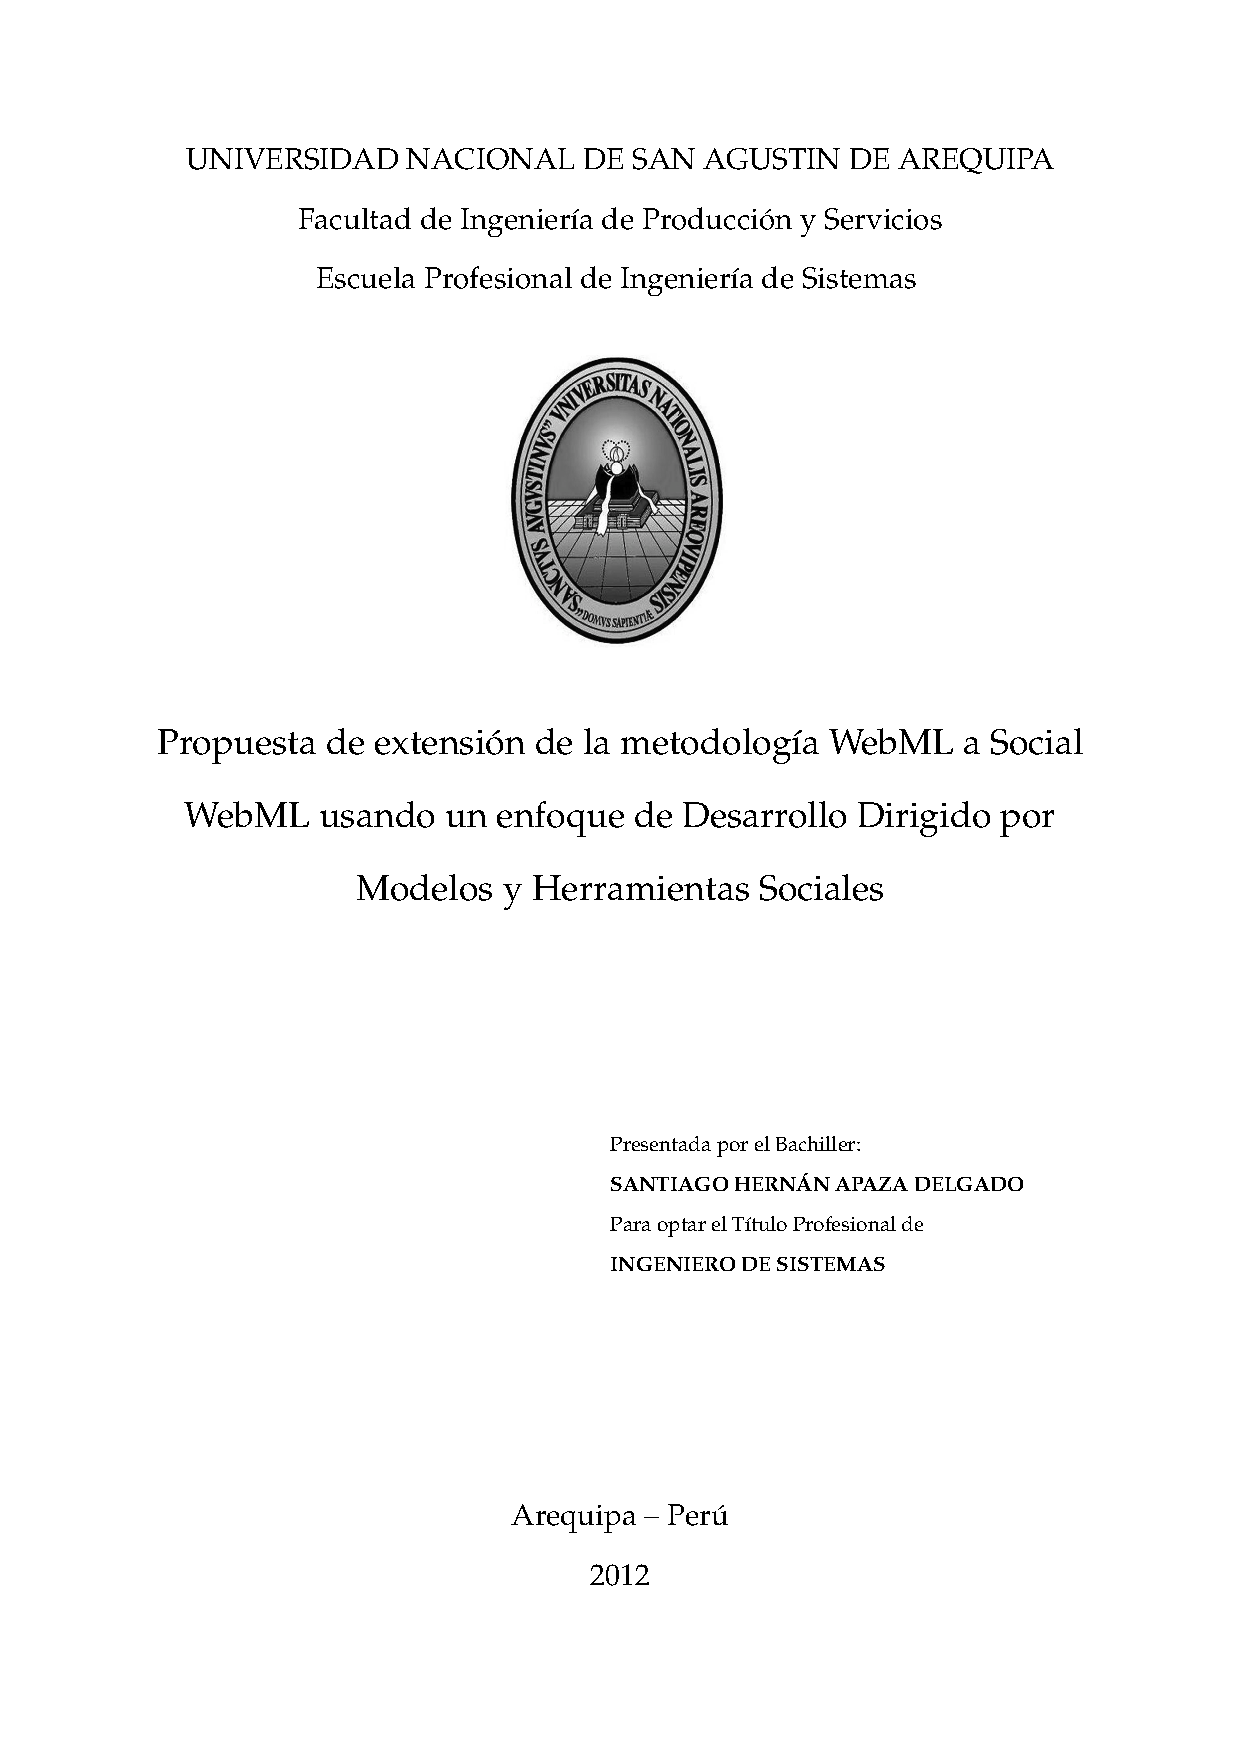
\includepdf[pages=1]{frontTitlePage/portada}
%\marginsize{4cm}{2.5cm}{2.5cm}{2.5cm}
\frontmatter
\pagestyle{plain}
   
%\hyphenation{} 
% Dedication
%\begin{epigraphs}
%  \qitem{
%    Dedicado a\ldots\ldots
%  }{\small Santiago Hern\'an Apaza Delgado}
%end{epigraphs}
 
% Acknowkedgements
%\chapter*{Reconocimientos}
%Gracias a\ldots\ldots

% Abstract (in English and Spanish)

\chapter*{RESUMEN}
\label{chap:abstract}

\textit{En este trabajo se presenta una propuesta para extender el lenguaje y
metodolog\'ia de desarrollo de aplicaciones basadas en web: WebML para que
con el uso del Desarrollo Dirigido por Modelos (MDD) y herramientas sociales,
en la cual prima el uso de las Redes Sociales, se pueda alcanzar el uso del
paradigma social y con el uso de un IDE se pueda generar de forma
autom\'atica aplicaciones \textbf{sociales} basadas en web y as\'i la existencia
de Social WebML.}



% Preface and conventions
\chapter*{Convenciones}
\label{chap:preface} 
En este cap\'itulo se enumeraran algunas convenciones l\'exicas, sint\'acticas y
tipogr\'aficas usadas en el presente documento.

\begin{comment}
\section*{Notations}
\label{sec:notations}
Lineas abajo se encuentra la lista de notaciones usadas en el documento,
con la explicaci\'on de su significado.
\end{comment}

\section*{Acr\'onimos}
\label{sec:acronyms}
Lineas abajo se encuentra la definici\'on de los acr\'onimos que aparecen
en el presente trabajo.

\begin{acronym} 
  \setlength{\itemsep}{0pt}\small
  \acro{COP}{\emph{Programaci\'on Orientada a Componentes (Component Oriented
  Programming)}}
  \acro{WebML}{\emph{Lenguaje de Modelado Web (Web Modeling Language)}}
  \acro{MDD}{\emph{Desarrollo Dirigido por Modelos (Model-Driven Development)}}
  \acro{MDA}{\emph{Arquitectura Dirigida por Modelos (Model-Driven
  Architecture)}}
  \acro{MDE}{\emph{Ingenier\'ia Dirigida por Modelos (Model-Driven
  Engineering)}} \acro{PIM}{\emph{Modelo Independiente de la Plataforma (Platform Independent
  Model)}}
  \acro{PDM}{\emph{Modelo de Definici\'on de la Plataforma (Platform
  Definition Model)}}
  \acro{PSM}{\emph{Modelo Espec\'ifico de la Plataforma (Platform Specific
  Model)}}
  \acro{DSL}{\emph{Lenguaje Espec\'ifico del Dominio (Domain Specific
  Language)}}
  \acro{CASE}{\emph{Ingenier\'ia de Software ayudada por Computadoras (Computer
  Aided Software Engineering)}}
  \acro{ERM}{\emph{Modelo Entidad--Relaci\'on (Entity-Relationship Model)}}
  \acro{UML}{\emph{Lenguaje de Modelado Unificado (Unified Modeling
  Language)}} 
  \acro{XML}{\emph{Lenguaje Extensible por Marcas (eXtensible Markup
  Language)}}
  \acro{OQL}{\emph{Lenguaje de Consulta de Objetos (Object Query Language)}}
  \acro{OCL}{\emph{Object Constraint Language}}
  \acro{RUP}{\emph{Rational Unified Process}}
  \acro{CRM}{\emph{Customer Relationship Manager}}
  \acro{FOAF}{\emph{Amigo de un Amigo (Friend Of A Friend)}}
  \acro{AJAX}{\emph{Asynchronous JavaScript And XML}}
  \acro{IDE}{\emph{Ambiente de Desarrollo Integrado (Integrated Development
  Environment)}}
  \acro{BPM}{\emph{Modelado de Procesos de Negocio (Business Process Modeling)}}
  \acro{NCM}{\emph{Modelo Conceptual de Navegaci\'on (Navigation Conceptual Model)}}
  \acro{ADM}{\emph{Modelo de Datos Araneus (Araneus Data Model)}}
  \acro{W3I3}{\emph{WWW Intelligent Information Infrastructure }}
\end{acronym}

% Lists
\clearpage
\tableofcontents
\clearpage
\listoffigures
\clearpage
\listoftables

% Main text
\mainmatter
\pagestyle{Ruled}

% Objective of the work
% Description of work done
% Main results and innovative aspects
% Outline of the thesis
\chapter{INTRODUCCI\'ON}
\label{chap:Introduction}
	\section{Planteamiento del problema}
	\label{sec:Problem}
	Hoy en d\'ia vivimos en un mundo considerado social, desde el \'ambito m\'as
	b\'asico de la interacci\'on f\'isica entre los mismos seres humanos y el
	ambiente que nos rodea hasta llegar inclusive a una interacci\'on ``virtual'',
	dentro de la cual en los \'ultimos a\~nos se ha notado un constante y r\'apido
	crecimiento; esto desde la aparici\'on de la Web 2.0 y su evoluci\'on 
	constante llegando incluso hasta hoy en d\'ia a hablar de una Web Social, en la
	cual subsisten y conviven los individuos sociales, los cuales, utilizan
	herramientas sociales (Wikis, blogs, etc.) entre ellas una de las m\'as
	importantes: Las Redes Sociales.
	 
	Con la aparici\'on de la Web 2.0 se cerr\'o una etapa en la historia de la
	Internet, ya que antes de ella se conoc\'ia \'unicamente una Internet de \'ambito
	informativo (el usuario solo pod\'ia acceder a la informaci\'on), y despu\'es del
	punto de quiebre dado por la Web 2.0 se dio comienzo al desarrollo de las
	denominadas aplicaciones basadas en web, en las cuales ya no se trataba
	de p\'aginas web, las cuales ten\'ian  \'unicamente por objetivo el acceso a
	informaci\'on, sino tambi\'en la de un intercambio, correcci\'on, valor
	a\~nadido, en otras palabras, una visi\'on de \'ambito interactivo (el usuario
	ya pod\'ia corregir, aportar, borrar, comentar, etc.)
 
	Al transcurrir el tiempo, analistas, dise\~nadores, desarrolladores, etc.
	comenzaron a notar que las herramientas de programaci\'on tradicionales, como por
	ejemplo \ac{UML}, \ac{RUP}, etc., no les ayudaban en muchos de los aspectos que
	este nuevo \'ambito de desarrollo conllevaba, como era la escalabilidad a niveles
	astron\'omicos, la concurrencia continua, las grandes cantidades de informaci\'on
	que se deb\'ia de manipular, y muchos otros aspectos los cuales pod\'ian no estar
	preconcebidos al momento del dise\~no pero que en el mundo real lo vivimos a cada
	instante; es por ello que se dise\~n\'o un lenguaje y metodolog\'ia adecuada para el
	desarrollo de aplicaciones basadas en web, el mismo que se nombr\'o como
	\ac{WebML}, con la aparici\'on de esta metodolog\'ia y lenguaje se pudo solucionar
	muchos aspectos del dise\~no, desarrollo, la misma forma de ver el ciclo de vida
	del desarrollo de una aplicaci\'on cambio de manera considerable.
	 
	Como se coment\'o inicialmente ahora vivimos el tiempo de la Web Social, y la
	metodolog\'ia y lenguaje \ac{WebML} al momento de ser concebida no previno la
	aparici\'on de una aplicaci\'on basada en web de tipo social como son por
	ejemplo las redes sociales o inclusive el uso de aquellas para brindar un valor
	a\~nadido a otras aplicaciones basadas en web, aunque gracias a una
	caracter\'istica que posee, es que se ha podido extender hacia otras ramas de
	desarrollo que no fueron pensadas de implementar un inicio, es por ello que
	se explotar\'a esta caracter\'istica para poder implementar el paradigma
	social en la metodolog\'ia y lenguaje \ac{WebML}
	
	\section{Justificaci\'on del problema}
	\label{sec:Justify}
	Tanto desde la implementaci\'on de una aplicaci\'on social basada en web como en su
	propia utilidad hacia y desde el usuario y due\~no de la aplicaci\'on son muchos
	los aspectos que difieren de una aplicaci\'on basada en web tradicional. Por
	ejemplo actualmente se puede notar la existencia de p\'aginas web, aplicaciones
	web y comunidades web, las cuales tienen por objetivo las de:
	\begin{itemize}
	  \item Informar de alguna determinada actividad a un grupo de usuarios.
	  \item Servir de apoyo a alguna determinada labor y sobre todo la
	  descentralizaci\'on del motor de actividades.
	  \item Mantener determinados lazos entre los individuos (usuarios) de la
	comunidad.
	\end{itemize}
	
	Aunque hoy en d\'ia se introduce parte de las comunidades en casi cualquier
	lugar no se est\'a logrando explotar y sobre todo llegar a acoger las
	caracter\'isticas de la web social. Es por ello que con la presente propuesta
	se persigue cubrir al menos los aspectos b\'asicos que se precisan para que
	desde su desarrollo hasta el momento de su liberaci\'on una aplicaci\'on basada
	en web sea considerada una aplicaci\'on ``social'' basada en web, las bases de
	nuestra propuesta estar\'an basadas en los conceptos brindados por \ac{WebML} y
	para el desarrollo de la misma se utilizar\'a un enfoque basado en Desarrollo
	Dirigido por Modelos para proveer modelos que puedan ser reutilizados y
	mejorados en posteriores proyectos.
	
	\section{Objetivos}
	\label{sec:Objectives}
	\begin{enumerate}
	  \item Objetivo General
	  
	  \begin{itemize}
	    \item Proponer la extensi\'on de la metodolog\'ia/lenguaje de desarrollo de
	    aplicaciones basadas en web (\ac{WebML}) a Social WebML para poder soportar
	    el paradigma Social.
	  \end{itemize}
	  
	  \item Objetivos espec\'ificos
	  
	  \begin{itemize}
	    %\item Proponer y dise\~nar plantillas de levantamiento de requisitos
	    %sociales.
	    \item Presentar una posible propuesta de uso espec\'ifico para los patrones
	    sociales de dise\~no.
	    \item Dise\~nar e implementar unidades de programaci\'on funcionales para el
	    desarrollo de aplicaciones sociales basadas en web.
	    \item Hacer uso de Herramientas Sociales en la extensi\'on del lenguaje de
	    desarrollo de aplicaciones basadas en web.
	  \end{itemize}
	  
	\end{enumerate}
	
	\section{Estado del Arte}
	\label{sec:Status}
	%%%%%se comenta%%%%%
	Como punto de partida se comenta el trabajo realizado por Gerosa et
	al.	en \cite{Gerosa2005}, en el cual se desarroll\'o una extensi\'on de la
	metodolog\'ia de desarrollo de software cl\'asico:
	Rational Unified Process denominada RUP3C llamada as\'i por: ``Cooperation,
	Comunication and Coordination'' procesos los cuales en este trabajo se defiende
	que son las bases para desarrollar una comunidad web la cual m\'as
	espec\'ificamente se basa en extender la fase de desarrollo haciendo uso de
	\ac{COP} y aspectos basados en las $3$ C's para
	dirigir el desarrollo de la comunidad de forma adecuada.
	
	Otro punto importante fue nombrado por Fraternali et al. en
	\cite{Fraternali2010} y Frattini y Silva en \cite{Frattini2007}, en los
	cuales se muestra un primer acercamiento a un \'ambito social a \ac{WebML}, en la cual
	esta es utilizada y en cierta forma extendida para el dise\~no e
	implementaci\'on de una comunidad web en la cual se describe los patrones de
	dise\~no sociales y ejemplos del uso de las mismas en algunas comunidades web
	actuales, as\'i como una descripci\'on a detalle de la metodolog\'ia \ac{WebML}
	como algunos puntos resaltantes a tomar en cuenta como aporte para el
	desarrollo de una comunidad web con \ac{WebML}.
	
	Desde el punto de vista nombrado en el p\'arrafo anterior
	Bozzon en \cite{Bozzon2009} propuso de forma te\'orica, el como debieran de
	comportarse los patrones de dise\~no sociales adem\'as de mostrar una
	implementaci\'on emp\'irica, desde una vista b\'asica hasta una vista complejo
	y ampliada de cada uno de los patrones sociales.
	
	De forma indirecta Brambilla en \cite{Brambilla2006} y Ceri et
	al. en \cite{Ceri2010} comenzaron a ampliar los trabajos propuestos
	anteriormente y a introducir un aspecto social en las metodolog\'ias
	comentadas, al proponer el uso de tecnolog\'ias, como por ejemplo \ac{AJAX}, en
	la auto--generaci\'on de aplicaciones basadas en web que ya posean un correcto
	dise\~no de requerimientos de negocio, el cual se realizaba con la
	metodolog\'ia \ac{BPM}, con lo cual se volv\'ia m\'as interactiva la relaci\'on
	existente entre el usuario y la aplicaci\'on generada.
	
	Brambilla et al. en \cite{Fraternali2011} propusieron una extensi\'on del
	\ac{BPM} en la cual las herramientas sociales juegan un papel muy importante en el
	aspecto de comunicaci\'on en un proceso de negocio, el cual es uno de los pilares
	que tomaremos al momento del desarrollo de la propuesta.
	
	\section{Metodolog\'ia del Trabajo}
	\label{sec:Methodology}
	La limitaci\'on m\'as resaltante en este proyecto son las diversas posturas que los
	autores toman al referirse o intentar definir lo que significa y por
	consiguiente que conlleva el t\'ermino ``social'' en el desarrollo de una
	aplicaci\'on social basada en web, con lo cual se podr\'ia no llegar a cubrir los
	aspectos que muchos autores consideren ``b\'asicos''.
	
	Una restricci\'on que es tanto a favor como en contra del desarrollo de este
	trabajo es el constante y r\'apido cambio tanto en tecnolog\'ias como en
	atributos dados al paradigma social, lo cual puede conllevar a facilidad en
	la captura del \textit{core} de los modelos a desarrollarse como en la variable
	complejidad que pueden llegar a tener la implementaci\'on de los mismos.
	
	\section{Organizaci\'on de la Tesis}
	\label{src:Organization}
	El presente trabajo est\'a organizado de la siguiente manera:
	
	\begin{enumerate}
	  %\item El Cap\'itulo I, muestra una introducci\'on a conceptos que ser\'an
	  %importantes a lo largo del proyecto, los cuales sientan las bases de
	  %conocimiento elemental para poder comprender, analizar y proyectar el
	  %objetivo principal del trabajo.
	  \item El Cap\'itulo \ref{chap:Process}, se mostrar\'a el \textit{Marco
	  Te\'orico} necesario para el desarrollo de este trabajo; desde una breve
	  explicaci\'on de la Web 2.0, la Web Social y Sem\'antica, as\'i como \ac{MDD}
	  y \ac{WebML} y para finalizar el cap\'itulo una breve rese\~na de algunos
	  trabajos relacionados a la propuesta presentada en este trabajo.
	  \item El Cap\'itulo \ref{chap:Proposal}, se presentar\'a la
	  \textit{Propuesta: Social WebML} en sus diferentes etapas, desde la etapa de
	  \textit{comunicaci\'on} hasta la etapa de \textit{construcci\'on}, dando un
	  breve hincapi\'e durante el cap\'itulo en algunos aspectos a tener en
	  consideraci\'on al momento de realizar cada etapa en el desarrollo de una
	  aplicaci\'on social basada en web.
	  \item El Cap\'itulo \ref{chap:studyCase}, se realizar\'a un \textit{Caso de
	  Estudio} did\'actico el cual tendr\'a por nombre \textit{WR Travel Agency} o
	  \textit{WRTA} en el cual se utilizar\'a la metodolog\'ia Social WebML para
	  brindar una soluci\'on a las necesidades sociales que esta tenga.
	  \item El Cap\'itulo \ref{chap:Conclusions}, se enumerar\'a las
	  \textit{Conclusiones} a las que se llego en el desarrollo del trabajo.
	\end{enumerate}

\chapter{MARCO TE\'ORICO}
\label{chap:Process}
	\section{Web 2.0}
	\label{sec:Web20}
	Como O'Reilly en \cite{OReilly2007} comenta: la web 2.0 aparece a partir de
	un punto tecnol\'ogico en el cual la web tradicional por s\'i misma ya no
	soportaba todas aquellas actividades que el usuario deseaba realizar, es por
	ello que se le a\~nadi\'o un conjunto de caracter\'isticas, ``necesarias m\'as
	no suficientes", para acomodarse a las necesidades del usuario, las cuales son
	acotadas y mejor entendidas por Frattini y Silva en \cite{Frattini2007},
	estas son enumeradas como sigue a continuaci\'on:
	
	%Caracter\'isticas
	\begin{enumerate}
	  \item La web como una plataforma - Esta caracter\'istica denota a la web
	  como una plataforma en la cual se puede a\~nadir servicios cada vez de mayor
	  complejidad\footnote{Actualmente \'esta caracter\'istica es mejor
	  entendida y/o conocida con el t\'ermino ``MashUp''}.
	  \item Aprovechar la inteligencia colectiva -  Esta caracter\'istica expresa
	  y/o define a la contribuci\'on de los usuarios como el recurso m\'as
	  importante a ser explotado.
	%Revisar nombre ingles/espa\~nol
	  \item Blogging\footnote{Es una forma sencilla y gratis de publicar en
	  Internet experiencias, comentarios, ideas, etc.} y la inteligencia de las
	  masas - Esta caracter\'istica define a las personas como los principales
	  actores, de los cuales siempre se tiene que tener en cuenta para las
	 decisiones a tomar.
	%Revisar nombre ingles/espa\~nol
	  \item Data as the next Intel Inside - Esta caracter\'istica expresa y/o
	  denota que la posesi\'on de la informaci\'on, la cual puede ser transformada
	  en oportunidades para las empresas.
	  \item Finalizaci\'on del concepto de \textit{ciclo de liberaci\'on de
	  software} - Esta caracter\'istica denota que el usuario final se
	  convertir\'ia en parte del equipo de desarrollo, jugando el papel de un
	  ``desarrollador'' y al mismo tiempo de tester\footnote{Actualmente el mayor
	  papel en la construcci\'on que realiza el usuario es como beta tester para
	  las liberaciones alfa y/o beta. Total Commander da un buen ejemplo de ello:
	  ``http://www.ghisler.com/800\_b23.php''}.
	%Revisar nombre ingles/espa\~nol
	  \item Lightweight programming model - Llegar a poseer una capacidad de mezcla
	  entre contenidos y servicios.
	  \item Software por encima del nivel de simples dispositivo - En esta
	  caracter\'istica se concibe la idea de descartar la PC en si misma y llegar
	  a la computaci\'on ubicua\footnote{Tambi\'en llamada ubicomp, en
	  la cual la interacci\'on con los componentes inform\'aticos no se llegue a
	  percibir estos como objetos diferenciados.}.
	%Revisar nombre ingles/espa\~nol
	  \item Rich user experience - Esta caracter\'istica m\'as como un consejo
	  de dise\~no se da en la frase: \textit{Los usuarios prefieren interfaces
	  f\'aciles de usar (esenciales y efectivas)}.
	\end{enumerate}
	
	Estas son las caracter\'isticas que O'Reilly en \cite{OReilly2007} propuso para
	comenzar una segunda etapa en la web, el cual con el pasar de los a\~nos los puntos
	antes nombrados se disgregaron y se especializaron, definiendo cada uno sus
	propios lineamientos.
%Agregar una referencia para el parrafo anterior.
	
	\section{Web Social y/o Web Semantic}
	\label{sec:SSWeb}
	Gruber en \cite{Gruber2008} coment\'o que la web social es representada por
	una clase de p\'aginas web y aplicaciones en un ecosistema de participaci\'on
	donde el ``valor'' es creado por la adici\'on de la contribuci\'on de muchos
	usuarios individuales, a lo cual Abu et al. en \cite{Bani2011} a\~nadieron que
	la participaci\'on de los usuarios se convierte en el principal generador de
	este valor y que la comunicaci\'on multi--direccional es aquella que crea
	conocimiento en el contexto de la conversaci\'on, en el cual se utiliza el
	conocido ``Sistema de Conocimiento Colectivo'' el cual es definido como la
	inteligencia colectiva m\'as una representaci\'on del conocimiento m\'as
	t\'ecnicas de razonamiento (tambi\'en llamado en este contexto: web
	sem\'antica).
	
	La web social es com\'unmente asociada a t\'erminos como inteligencia colectiva
	(collective intelligence) o sabidur\'ia de multitudes (wisdom of crowds) la
	cual esta basada en una arquitectura de participaci\'on y contribuci\'on
	colectiva, estos son considerados por Arroyo en \cite{Arroyo2007} como los
	principios de la web social y adem\'as los pilares para una nueva forma de
	construir p\'aginas web para permitir participaci\'on de gran n\'umero de
	usuarios. Adem\'as considera que la web se est\'a haciendo cada vez m\'as
	social ya que se est\'a dirigiendo cada vez m\'as a una larga cola de usuarios
	y todo esto gracias a que los servicios son cada vez m\'as f\'aciles de emplear
	y es por ello que Garcia-Molina et al. en \cite{Heymann2007} comentan que poco
	a poco la web social debe adoptar ciertos criterios, como convertirse en una
	unidad controladora (un administrador) en la cual la interacci\'on este bien
	definida entre los usuarios, los cuales deber\'ian de adoptar una forma de
	identificaci\'on \'unica, lo cual les brindar\'ia una identidad y sobre todo 
	que el acceso a la informaci\'on sea de f\'acil entrada para lo cual debiera de
	existir m\'ultiples interfaces (como por ejemplo las nubes de
	palabras\footnote{Tambi\'en conocidas como nube de tags o tag cloud, en la cual
	s representa de forma visual enlaces hacia distintos contenidos enlazados
	mediante las palabras existentes en la nube de tags}).

	Arroyo en \cite{Arroyo2007} y Garcia-Molina et al. en \cite{Heymann2007}
	plantearon una filosof\'ia para la Web Social, en la cual esta signifique
	que compartan recursos a la vez que se beneficia incluso a\'un m\'as de los
	recursos compartidos por otros, de esta forma la web se convertir\'ia en una
	plataforma de servicios en el sentido en que las p\'aginas web con esa
	filosof\'ia constituyan un espacio para que el usuario pueda participar
	a\~nadiendo contenidos de distintos tipos (mientras m\'as personas usen este
	servicio, este mejora) y para ello se tienen algunas caracter\'isticas
	representativas, como son:
	
	\begin{itemize}
	  \item Participaci\'on y colaboraci\'on del usuario
	  \item Incremento en los canales de comunicaci\'on
	  \item Interacci\'on
	  \item Compartir recursos y conocimientos (la meta es el beneficio mutuo)
	  \item Democracia (el usuario es el verdadero due\~no)
	  \item Car\'acter p\'ublico y abierto(f\'acil e intuitivo)
	  \item Obra colectiva (Por ejemplo Wikipedia)
	\end{itemize}
	
	Davies y Mintz en \cite{Davies2009} comentaron que las caracter\'isticas
	de la web social adicional a las anteriormente nombradas tambi\'en son:
	
	\begin{itemize}
	  \item El contenido social es generado por el usuario (mediante la
	  publicaci\'on de contenido)
	  \item Existencia de la facultad de poder crear y/o pertenecer a un grupo
	  (actualmente llamado: social networking)
	  \item Existencia de una plataforma cruzada en la cual los archivos son
	  compartidos (esta caracter\'istica es compartida con alguna de las
	  caracter\'isticas de la web sem\'antica en la cual se a\~nade que estos archivos
	  u objetos deben de ser compartidos con otras p\'aginas).
	  \item Unidades independientes de la p\'agina.
	  \item Los sub--segmentos\footnote{Como Davies y Mintz en \cite{Davies2009}
	  comentan, un sub--segmento es una porci\'on de contenido, o unidad de
	  programaci\'on, la cual puede ser referenciada independientemente de otras
	  unidades.} deben de ser completamente orientables (llamado fully
	  pointability), lo cual significa que una unidad puede apuntar hacia otra
	  unidad o hacia otro segmento.
	\end{itemize}
	
	Davies y Mintz en \cite{Davies2009} comentaron que de todas las
	caracter\'isticas antes nombradas y otra que pudieran encontrarse con el tiempo
	una de entre todas ellas se considerar\'ia el pilar de la web social, aquella
	que a diferencia de las otras tiene que existir, siendo esta: la
	caracter\'istica de la \textbf{contribuci\'on}.
	
	Adem\'as algo importante que comenta Abu et al. en
	\cite{Bani2011} es que con el crecimiento de la web social, se tienen millones
	de personas las cuales ofertan su conocimiento on--line lo cual significa que
	la informaci\'on es almacenada, buscable y f\'acilmente compartida; y un gran
	reto para la siguiente generaci\'on de la web sem\'antica y web social es
	encontrar el correcto emparejamiento entre lo que es puesto on--line y los
	m\'etodos para hacer \'util el razonamiento con la data. La verdadera
	inteligencia colectiva puede emerger si la data recolectada de todas las
	personas es agregada y recombinada para crear nuevos conocimientos y nuevas
	formas de aprender que los individuos humanos no pueden hacer por ellos mismos.
	
	%%%%%%%%%%%%%%%%%%%%%%%%%%%%%%%%%%%%%%%%
	\begin{figure}[here]
		\centering
		\caption{The FAQ--o--sphere}
		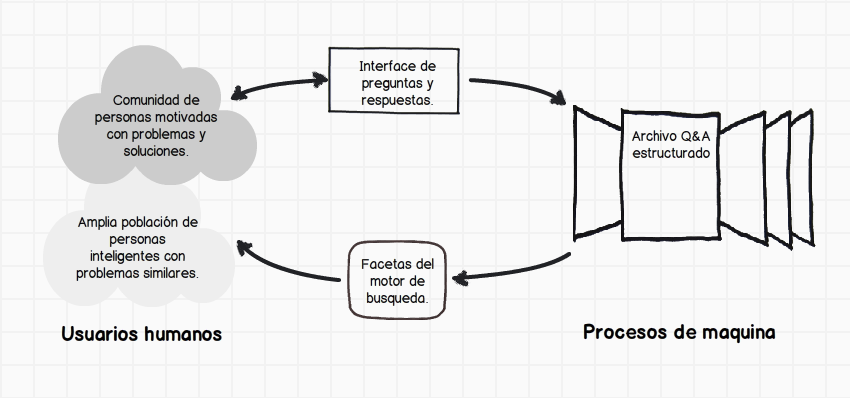
\includegraphics[width=0.9\textwidth]{figure/fig_faqosphere.png}
		\newline
		\textbf{Fuente:} Elaboraci\'on propia basada en: \textit{The
		FAQ--o--Sphere, an example of a collective knowledge system} visto por Gruber
		en \cite{Gruber2008}, p\'agina 4, Figura 1.
		\label{fig:FAQoSphere}
	\end{figure}
	 
	Sobre este contexto se desarrollaron algunas propuestas como son:
	\begin{itemize}
	  \item [a.] FAQ--o--sphere: El cual era un sistema experto que como se puede
	  ver en la Figura \ref{fig:FAQoSphere}, \'esta consume la data de una determinada
	  problem\'atica, recolectada de un conjunto de individuos y se realiza un
	  matching con un conjunto, c\'umulo o banco de problemas y desde las cuales da
	  una lista de aserciones similares. Es aqu\'i en donde ``Collected to
	  collective intelligence'' defin\'ia algunas restricciones que se deb\'ian de
	  considerar, como por ejemplo.
	  
	  \begin{itemize}
	    \item Conocimiento emergente: El cual deb\'ia de crearse desde el sistema,
	    considerando este tipo de conocimiento como nuevos.
	    \item Contenido inicial debe ser generado por el usuario.
	    \item Existencia de una sinergia humano/maquina, cuya combinaci\'on
	    proveer\'ia la capacidad de generar informaci\'on \'util que no puede ser
	    obtenida de otra forma.
	    \item Rendimiento creciente y a escala. 
	  \end{itemize}  
	    
	  \begin{figure}[here]
		\centering
		\caption{Conocimiento Colectivo: Real Travel}
		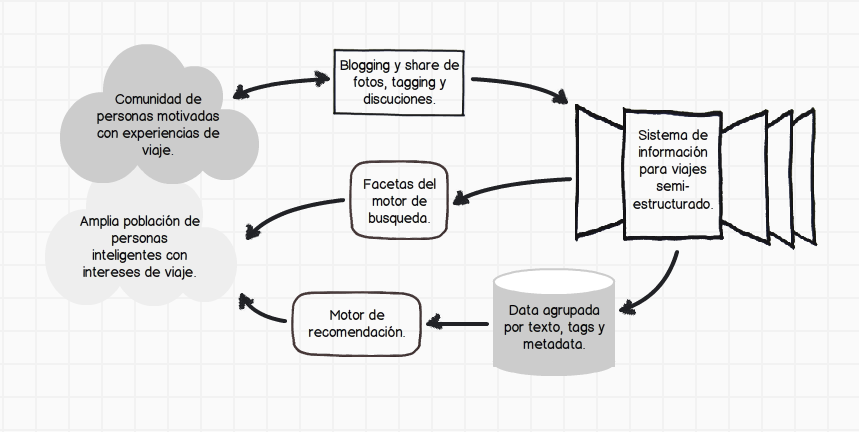
\includegraphics[width=0.9\textwidth]{figure/fig_realTravel.png} 
		\newline
		\textbf{Fuente:} Elaboraci\'on propia basada en: \textit{A collective
		knowledge system for travel} visto por Gruber en \cite{Gruber2008}, p\'agina
		14, Figura 2.
		\label{fig:realTravel}
	  \end{figure}
	
	  \item [b.] Real Travel: En esta propuesta se ve algunas similitudes con
	  respecto al modelo anterior los cuales se muestran en la Figura
	  \ref{fig:realTravel} y se explican a continuaci\'on.
	  
	  \begin{itemize}
	    \item Contenido real debe de ser hecho por los propios autores, el cual se
	    asemeja a la restricci\'on de que \textit{``El contenido inicial debe ser
	    generado por el usuario''}.
	    \item Debe lograrse una equivalencia a preguntar a los usuarios sobre sus
	    experiencias, el cual se asemeja conceptualmente a la restricci\'on de
	    \textit{``Existencia de una sinergia humano/maquina''}.
	    \item Se puede cubrir las necesidades y dar mayores soluciones a sus
	    problemas
	  \end{itemize} 
	  
	\end{itemize}
	

%%%%%%%%%%%%%%%%%%%%%%%%%%%%%%
	Estos modelos se basan en fomentar la contribuci\'on con la cual se
	incrementar\'ia los retornos con escalas y como resultado de estas condiciones
	se lograr\'ia un conocimiento emergente, pero este ya no ser\'ia generado por
	humanos sino inferido por el computador.
	
		\subsection{5 eras de la web social}
		\label{ssec:5eras}
		Se coment\'o la importancia de el poder identificarse de una manera
		\'unica en todo este mundo virtual llamado Internet, pero
		Owyang en \cite{Owyang2009} coment\'o que el uso de los ID's, representa solo
		el comienzo de la transformaci\'on en que la web evolucionar\'a paso a paso
		desde p\'aginas web sociales separadas, concebidas como islas por
		Panzer y Smarr en \cite{Smarr2010}, hacia una experiencia social compartida.
		Es por ello que Owyang en \cite{Forrester2009} coment\'o que
		para poder referirse a la web social se tiene que referirse a alg\'un tiempo
		en especial, los cuales se han dividido en un total de $5$ etapas de tiempo,
		cada una bien diferenciada del anterior y del posterior; a continuaci\'on se
		describir\'a cada una resaltando lo m\'as importante de cada era para poder
		entender como se deber\'ia de evolucionar en el desarrollo de la
		web social.
		
		%\begin{figure}[here]
		%	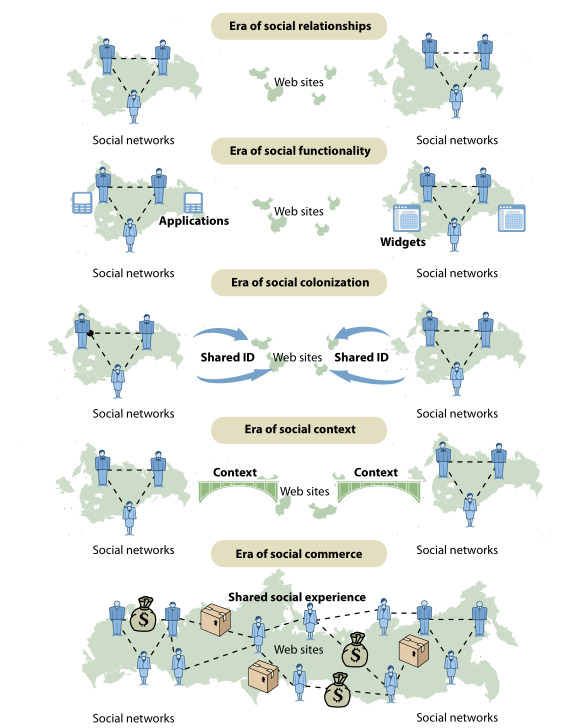
\includegraphics[width=0.9\textwidth]{figure/fig_5Eras.png}
		%	\caption{Las 5 eras de la Social Web}
		%	\label{fig:5Eras}
		%\end{figure}
	
		\begin{enumerate}
		  \item Era de las relaciones sociales (a\~nos $90$): Como se ve en la Figura
		  \ref{fig:5ErasA} en esta era las personas est\'an relacionadas y/o
		  conectadas a otras y comparten informaci\'on en lo que se consideran comunidades.
		  
		  \begin{figure}[here]
			\centering
			\caption{Las 5 eras de la Social Web -- Relaciones Sociales}
			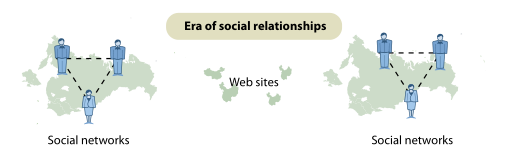
\includegraphics[width=0.9\textwidth]{figure/fig_5ErasA.png}
			\newline
			\textbf{Fuente:} \textit{The Five Eras Of The Social Web}, visto por Owyang
			en \cite{Forrester2009}, p\'agina 3, Figura 1.
			\label{fig:5ErasA}
		  \end{figure}
		
		  \item Era de la funcionalidad social: Como se ve en la Figura
		  \ref{fig:5ErasB} en esta era, el foco permanece en las actividades que se
		  realizan en las redes sociales las cuales consiguen hacer evolucionar a las
		  redes sociales a plataformas, las cuales soportan aplicaciones sociales
		  interactivas y estas son consideradas ``Sistemas operativos''. La tecnolog\'ia
		  en esta era entra en un creciente auge, pero teniendo un punto en contra lo
		  cual le pone un cota superior a su evoluci\'on y es que la tecnolog\'ia
		  subyacente solamente existe y persiste aun dentro de cada isla que se crea
		  dentro de cada red social, como se ve en la Figura \ref{fig:SNMap} estas
		  islas aunque comparten un mismo lugar de residencia (Internet), estas no se
		  relacionan de manera alguna, lo cual conllevar\'ia seg\'un Panzer y Smarr en
		  \cite{Smarr2010} a su posterior desaparici\'on.
		  
		  \begin{figure}[here]
			\centering
			\caption{Las 5 eras de la Social Web -- Funcionalidad Social}
			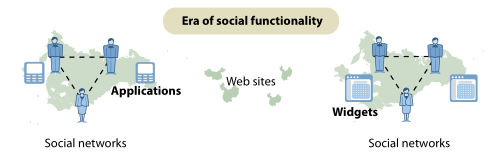
\includegraphics[width=0.9\textwidth]{figure/fig_5ErasB.png}
			\newline
			\textbf{Fuente:} \textit{The Five Eras Of The Social Web}, visto por Owyang
			en \cite{Forrester2009}, p\'agina 3, Figura 1.
			\label{fig:5ErasB}
		\end{figure}
		
		  Algunos aspectos representativos de esta era son:
		
		  \begin{itemize}
		    \item Los consumidores comparten sus experiencias, pero no pueden
		    conectarlas a trav\'es de las redes.
		    \item Aunque la evoluci\'on de las redes sociales se considera elevado y
		    r\'apido posee un l\'imite que es el alcance de su comunicaci\'on, pero para
		    esto comienza a surgir intentos para eliminar esta barrera, como son
		    \textit{Facebook Connect, O'Auth}, etc.
		    \item Las marcas comerciales se conectan con perfiles pero no pueden
		    alcanzar a toda la audiencia.
		  \end{itemize}
		  
		  \begin{figure}[here]
			\centering
			\caption{Mapa relativo de las Redes Sociales}
			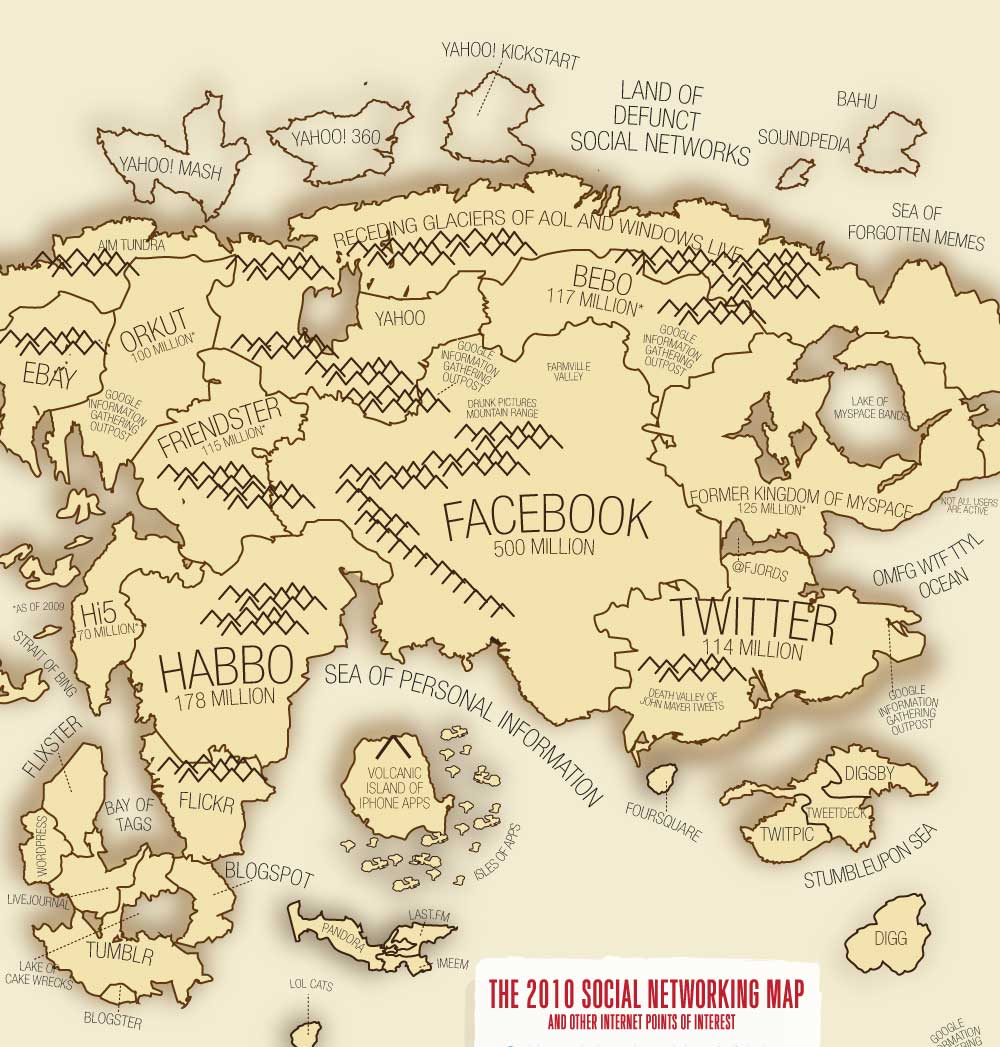
\includegraphics[width=0.7\textwidth]{figure/fig_SocialNetworkMap.png}
			
			\label{fig:SNMap}
		  \end{figure}
		
		  En conclusi\'on esta era posee una gran barrera que son las mismas islas que
		  hace que esta crezca tan r\'apida y esplendorosamente.
		    
		    
		  \begin{figure}[here]
			\centering
			\caption{Las 5 eras de la Social Web -- Colonizaci\'on Social}
			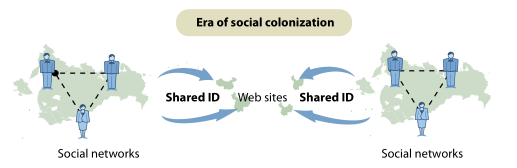
\includegraphics[width=0.9\textwidth]{figure/fig_5ErasC.png}
			\newline
			\textbf{Fuente:} \textit{The Five Eras Of The Social Web}, visto por Owyang
			en \cite{Forrester2009}, p\'agina 3, Figura 1.
			\label{fig:5ErasC}
		  \end{figure}
		
		  \item Era de la colonizaci\'on social ($2009$ en adelante): Como se ve en la Figura
		  \ref{fig:5ErasC} en esta era cada experiencia puede ser ahora social gracias
		  a que nuestra identidad puede migrar de un lugar a otro. Esto se realiza
		  gracias a: \textit{O'Auth} o \textit{Facebook Connect}. Las
		  caracter\'isticas m\'as resultantes en esta era son:
		  \begin{itemize}
		    \item Los usuarios, consumidores, clientes, etc. pueden navegar en la web
		    sin el sentimiento de una experiencia solitaria ya que gracias a tener
		    una identidad \'unica pueden encontrar a sus ``amigos'' donde sea que
		    ellos se encuentren. Un ejemplo sencillo es que ellos podr\'an ver
		    p\'aginas creadas y/o recomendadas por sus amigos en la \textit{``isla''}
		    donde ellos se encuentren.
		    \item Para a\~nadir valor, las redes sociales agregan actividades de
		    miembros a su red. Por ejemplo en la Figura \ref{fig:Biography}
		    vemos como \textit{Facebook} lo representa mediante una presentaci\'on en
		    \textit{biografia} o \textit{timeline}\footnote{www.facebook.com} en la
		    cual se puede ver como re\'une en un solo sitio y de manera organizada los
		    aspectos que Facebook considero de mayor relevancia para sus usuarios.
		    \item Se crea un cambio radical desde un marketing de forma
		    ``tradicional'' a un marketing mediante ``recomendaciones sociales''.
		  \end{itemize}

		  \begin{figure}[here]
			\centering
			\caption{Facebook: Modo Timeline o Biography}
			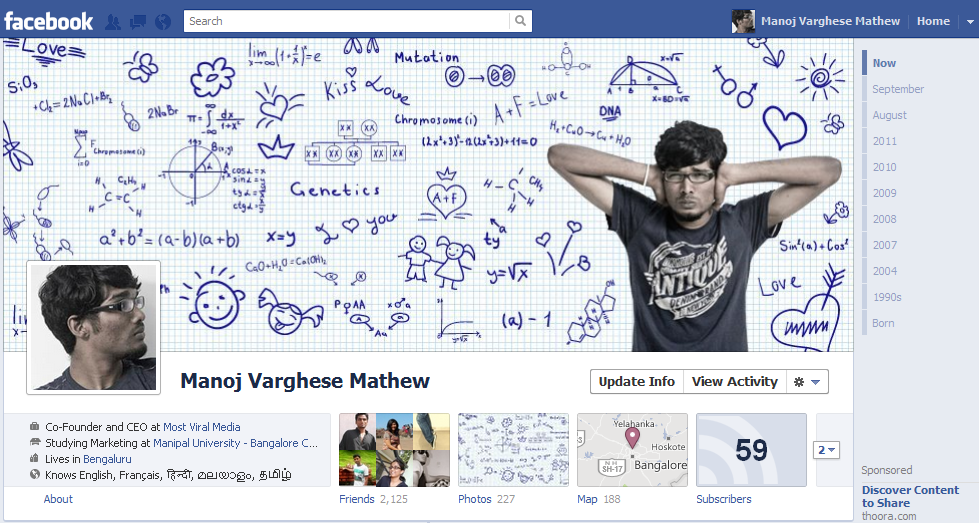
\includegraphics[width=0.9\textwidth]{figure/fig_biography.png}
			
			\label{fig:Biography}
		  \end{figure}
		  
		  
		\begin{figure}[here]
			\centering
			\caption{Las 5 eras de la Social Web -- Contexto Social}
			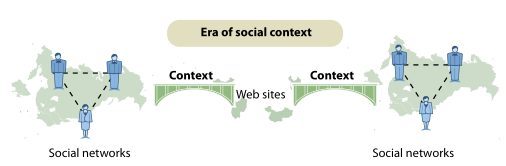
\includegraphics[width=0.9\textwidth]{figure/fig_5ErasD.png}
			\newline
			\textbf{Fuente:} \textit{The Five Eras Of The Social Web}, visto por Owyang
			en \cite{Forrester2009}, p\'agina 3, Figura 1.
			\label{fig:5ErasD}
		\end{figure}
		
		  \item Era del contexto social ($2010$ en adelante): Como se ve en la Figura
		  \ref{fig:5ErasD} el contenido personalizado y preciso, desde las redes
		  sociales, gracias a la experiencia del usuario basado en sus preferencias,
		  su comportamiento y sus amigos. En esta era se logra la tan anhelada
		  identidad portable, no solo restringi\'endonos a informaci\'on personal sino
		  tambi\'en a experiencias, demograf\'ia e historia.
		  Otras caracter\'isticas importantes de esta era son:
		  
		  \begin{itemize}
		    \item El usuario dependiendo de la situaci\'on expondr\'a informaci\'on
		    relevante asociada a su ID, a las p\'aginas web que visite.
		    \item Las redes sociales cambiaran su modelo de negocios.
		    \item Las marcas comerciales personalizar\'an sus p\'aginas web para
		    impulsar los resultados, realizando de esta forma un marketing de tipo
		    ad--hoc para cada usuario.
		    \item Los resultados de la b\'usqueda ser\'an de contenido basado en
		    relevancia social de forma que la informaci\'on ser\'a m\'as r\'apida y relevante
		    al momento de b\'usqueda.
		    \item Los dispositivos m\'oviles permiten a cualquiera tener un entorno en
		    el bolsillo.
		    \item Los proveedores de TV enlazar\'an el aspecto social con la web
		    tradicional generando as\'i la televisi\'on Social. Un ejemplo de una
		    tecnolog\'ia que poco a poco busca este objetivo en la actualidad
		    es Apple TV\footnote{http://www.apple.com/es/appletv/}.
		  \end{itemize}
		    
		    
		\begin{figure}[here]
			\centering
			\caption{Las 5 eras de la Social Web -- Comercio Social}
			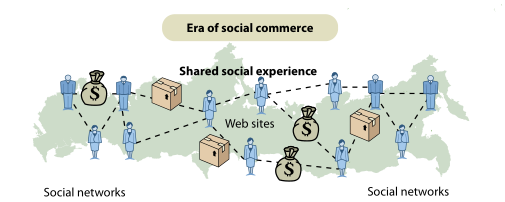
\includegraphics[width=0.9\textwidth]{figure/fig_5ErasE.png}
			\newline
			\textbf{Fuente:} \textit{The Five Eras Of The Social Web}, visto por Owyang
			en \cite{Forrester2009}, p\'agina 3, Figura 1.
			\label{fig:5ErasE}
		\end{figure}
		
		
		  \item Era del comercio social: Como se ve en la Figura
		  \ref{fig:5ErasE} las comunidades definen productos y servicios
		  futuros, manejando as\'i la innovaci\'on y por consiguiente convirti\'endose en
		  repositorios de identidades y relaciones. Algunas caracter\'isticas de esta
		  era son:
		  
		  \begin{itemize}
		    \item Los usuarios dejar\'an que las comunidades tome el control sobre lo
		    que compran.
		    \item Las redes sociales se convertir\'an en la siguiente generaci\'on de
		    sistemas \ac{CRM} (Por ejemplo SalesForte\footnote{http://salesforte.com/})
		    \item Los formularios de registro desaparecer\'an y el contenido estar\'a
		    fragmentado.
		    \item La privacidad se convertir\'a en un gran reto y a la vez en un gran
		    punto de crecimiento sostenible ya que mientras m\'as seguridad exista
		    sobre un determinada p\'agina  web, la conexi\'on entre esta y una
		    marca comercial ser\'a m\'as fuerte y por consiguiente m\'as confiable de
		    elecci\'on por el usuario.
		    \item Una sobre exposici\'on causar\'a el retiro de las redes sociales de
		    vez en cuando.
		    \item Las redes sociales tendr\'an como necesidad fundamental, el
		    reforzar seriamente sus capacidades de tratamiento de datos.
		  \end{itemize}
% Anhadir porque se supone estos
		Aunque en la actualidad se deber\'ia de estar en la $4^a$ 
		era, relativamente se est\'a a mediados de la $3^a$.
		\end{enumerate}
		
		\subsection{Desarrollo de Aplicaciones Sociales}
		\label{sec:DevelopingSA}
		Para poder desarrollar aplicaciones sociales primero debe hablarse
		sobre la concepci\'on, planteamiento y producci\'on de sitios web y aplicaciones
		que soportan la interacci\'on social. Porter en \cite{Porter2008} le llama
		``Dise\~no Social'' y comenta que el reto del software social es la
		problem\'atica del dise\~no de interfaces que sean flexibles \'osea que
		soporten el comportamiento social actual y deseado de las personas que lo
		usan. Porter en \cite{Porter2008} acota una frase muy especial.
		
		\begin{quotation}
		\textit{Solo los seres humanos son sociales por lo tanto nuestro software
		tambi\'en debe serlo.}
		\end{quotation}
		
		Al momento de desarrollar aplicaciones sociales se debe tener algunas
		consideraciones como por ejemplo:
		
		Abu et al. en \cite{Bani2011} comenta el como debiera de ser el ambiente del
		desarrollo social, el cual considera que debiera tener herramientas de programaci\'on
		colaborativa en tiempo real con caracter\'isticas de redes sociales integradas,
		con el cual se proveer\'ia un amplio rango  de facilidades para colaboraci\'on
		s\'incrona, as\'incrona y ``compartici\'on de informaci\'on entre miembros del
		equipo''. Y define al ambiente de desarrollo social como un espacio virtual
		donde los desarrolladores de un proyecto se inter--relacionan, por ejemplo
		algo que se deber\'ia tener en cuenta al momento del desarrollo de las
		aplicaciones es lograr lo que Porter en \cite{Porter2008} denomina
		\textit{Efecto Amazon} en la cual nos comenta que las personas van primero a
		un lugar, no para adquirir directamente lo que quieren, sino para hacer un
		estudio, ya que socialmente hablando lo que a las personas les gusta no
		generalmente es el producto, sino el conocimiento que se obtiene del mismo. Y
		siendo el caso que de verdad deseen la posesi\'on del producto, se detect\'o
		una actitud un poco extra\~na la cual era b\'asicamente que las personas
		buscan los defectos de aquellos productos que buscan, y de esta forma saber si
		estos productos tendr\'an alg\'un tipo de contradicci\'on contra lo que la
		marca comercial ofrece y lo que ellos desean.
		
		Tambi\'en nos habla sobre el efecto magn\'etico, nombrado as\'i ya que se basa
		simplemente en mantener a una persona el mayor tiempo posible navegando en la
		misma p\'agina, nos comenta que un buen ejemplo de esto es la utilizaci\'on de
		p\'aginas extremadamente grandes o como lo hace actualmente Facebook con el
		uso de p\'aginas sin fin, como se ve en la Figura \ref{fig:amazon}.
		Tambi\'en se pone \'enfasis en la comunicaci\'on de la forma ``Comentario'',
		ya que este logra concebirse como la informaci\'on m\'as pura que puede
		obtenerse de las personas, ya que este se obtiene:
		
		\begin{figure}[here]
			\centering
			\caption{Efecto Magn\'etico -- P\'agina sin fin}
			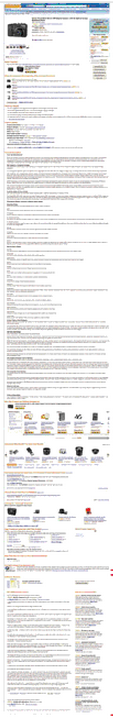
\includegraphics[width=0.2\textwidth]{figure/fig_amazon.PNG}
			\newline
			\textbf{Fuente:} Basado en el ejemplo del efecto magn\'etico visto por
			Porter en \cite{Porter2008}, p\'agina 3, Figura 1.1 (originalmente
			trabajado con Amazon pero en este caso visto en el caso de Facebook).
			\label{fig:amazon}
		\end{figure}
		
		\begin{itemize}
		  \item Sin realizar pago alguno
		  \item Hace que la referencia al objeto sea m\'inima
		  \item Logra alcanzar mayor atenci\'on del usuario 
		\end{itemize}
		
		\begin{figure}[here]
			\centering
			\caption{Comunicaci\'on Unidireccional}
			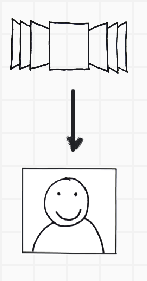
\includegraphics[width=0.3\textwidth]{figure/fig_onewayCommunication.PNG}
			\newline
			\textbf{Fuente:} Elaboraci\'on propia basada en \textit{The evolution of
			communication from one-way to many-way on the web}, visto por Porter en
			\cite{Porter2008}, p\'agina 15, Figura 1.2.
			\label{fig:oneWayCommunication}
		\end{figure}
		
		\begin{figure}[here]
			\centering
			\caption{Comunicaci\'on Bidireccional}
			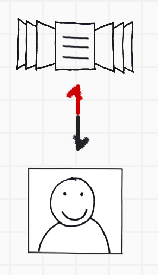
\includegraphics[width=0.3\textwidth]{figure/fig_twowayCommunication.PNG}
			\newline
			\textbf{Fuente:} Elaboraci\'on propia basada en \textit{The evolution of
			communication from one-way to many-way on the web}, visto por Porter en
			\cite{Porter2008}, p\'agina 15, Figura 1.2.
			\label{fig:twoWayCommunication}
		\end{figure}
		
		\begin{figure}[here]
			\centering
			\caption{Comunicaci\'on Many--to--Many o multi--direccional}
			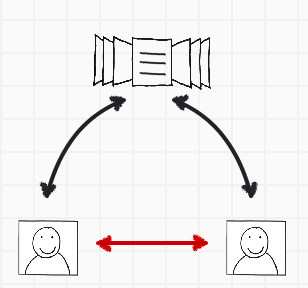
\includegraphics[width=0.5\textwidth]{figure/fig_manywayCommunication.PNG}
			\newline
			\textbf{Fuente:} Elaboraci\'on propia basada en \textit{The evolution of
			communication from one-way to many-way on the web}, visto por Porter en
			\cite{Porter2008}, p\'agina 15, Figura 1.2.
			\label{fig:ManyWayCommunication}
		\end{figure}
	 
		Adicionalmente se tendr\'ia que conversar sobre el t\'ermino
		comunicaci\'on, ya que de esto nace la socializaci\'on de una aplicaci\'on
		web; a continuaci\'on se muestra los tipos de comunicaci\'on los cuales Porter
		en \cite{Porter2008} utiliz\'o para diferenciar web tradicional, web 2.0 y la
		web social; que, como se puede notar en la Figura
		\ref{fig:oneWayCommunication} la comunicaci\'on \'unicamente proven\'ia de la
		p\'agina web, hacia el usuario; en la Figura \ref{fig:twoWayCommunication} se
		logra romper el esquema anterior y se consigue la bi--direccionalidad de la
		p\'agina web--usuario y viceversa y en la Figura 
		\ref{fig:ManyWayCommunication} en la cual la comunicaci\'on gracias a
		diferentes medios, como por ejemplo las redes sociales, se da p\'agina
		web--usuario y viceversa y adicionalmente una comunicaci\'on usuario--usuario.
		
		Entre estos tipos de comunicaci\'on, se busca un tipo de aplicaci\'on
		com\'unmente llamada ``Aplicaci\'on sofisticada'' en la cual Kamthan en
		\cite{Kamthan2009} a\~nade que en este tipo de interacci\'on se les considera
		a las personas como si estas fuesen un tipo de tecnolog\'ias primarias y/o
		secundarias y la web solamente un broker\footnote{Entidad que act\'ua como
		intermediario entre una entidad productora y una entidad consumidora.},
		adem\'as de considerarla como uno de los factores primarios para la visi\'on
		de la web social junto con la ``madurez de la infraestructura
		tecnol\'ogica y la disponibilidad del mismo en c\'odigo abierto'' y la
		``participaci\'on del p\'ublico en general a gran escala''.
		
		A partir de lo nombrado anteriormente se puede revisar los tipos de
		conversaci\'on:
		\begin{itemize}
		  \item Early/static: P\'aginas web con contenido est\'atico (con el que las
		  personas no pueden interactuar), esto se ve de forma m\'as clara en
		  la Figura \ref{fig:oneWayCommunication} en la cual la
		  informaci\'on viaja desde las p\'aginas web hacia el usuario.
		  \item Early web applications: El contenido es din\'amico y privado, el cual
		  cambia basada en las entradas del usuario, la comunicaci\'on entre
		  la aplicaci\'on y las personas, esto se ve de forma m\'as clara en
		  la Figura \ref{fig:twoWayCommunication} donde se muestra como la informaci\'on
		  va desde la p\'agina web al usuario y viceversa.
		  \item Share easily: Social web application: Contenido p\'ublico din\'amico
		  que cambia seg\'un la entrada de muchas personas, esto se ve de forma m\'as
		  clara en la Figura \ref{fig:ManyWayCommunication} donde la informaci\'on
		  viaja tambi\'en entre los mismos usuarios en conjunto con las p\'aginas web,
		  sus caracter\'isticas seg\'un Kamthan en \cite{Kamthan2009} son:
		  
		  \begin{itemize}
		  	\item Enfoque en la actividad primaria (?`para qu\'e interact\'uan?)
		  	\item Identificaci\'on de objetos sociales (?`con qu\'e interact\'uan?)
		  	\item Capacidad de elegir el core de las caracter\'isticas (acciones)
		  \end{itemize}
		\end{itemize}
		
	\section{Desarrollo Dirigido por Modelos}
	\label{sec:MDD}
	Cohen en \cite{Cohen2008} coment\'o que por los a\~nos $80$'s algunas de las
	compa\~n\'ias m\'as representativas a nivel mundial, como por ejemplo
	Integrated Development Environments (IDE - StP), Higher Order Software (ahora
	conocida como Hamilton Technologies, Inc., HTI), incursionaron por primera vez
	en el campo del \ac{MDE} con la propuesta de \ac{MDD} que con los a\~nos se
	convertir\'ia en una metodolog\'ia de desarrollo de software enfocada en el
	dise\~no de modelos y/o abstracciones, los cuales se acercar\'ian en mayor
	medida a los conceptos de alg\'un dominio en particular, m\'as que a conceptos de
	computaci\'on como algoritmos. Esto significaba incrementar la productividad al maximizar la
	compatibilidad entre sistemas, simplificando el proceso de dise\~no y
	promoviendo la comunicaci\'on entre individuos y equipos de trabajo en el
	sistema, Frattini y Silva en \cite{Frattini2007} comenta que las
	funcionalidades del mismo pueden primero ser definidas como un \ac{PIM}, despu\'es de lo cual se comienza
	a pensar reci\'en en un \ac{PDM} correspondiente a la aplicaci\'on web, el
	\ac{PIM} puede ser traducido a uno o m\'as \ac{PSM} para la implementaci\'on deseada. En
	este contexto se defini\'o una \ac{MDA}, en espec\'ifico no se refiere a los
	componentes del sistema, sino al dise\~no que lo dirige y en este los
	requerimientos funcionales y/o casos de uso, mientras tanto que la arquitectura
	propiamente dicha la provee la infraestructura a trav\'es de requerimientos no
	funcionales.
	
	Frattini y Silva en \cite{Frattini2007} resalt\'o que en el \ac{MDD} los
	elementos clave son aquellos que expresan los resultados de las diferentes actividades a
	desarrollarse y estos son los mismos modelos.
	Que el nivel de abstracci\'on en el desarrollo de software debe ser llevado a
	un nivel de modelo, los cuales separen los requerimientos funcionales y su
	implementaci\'on de los aspectos no funcionales y otros.
	
	\begin{figure}[here]
		\centering
		\caption{Proceso: Model-Driven Development}
		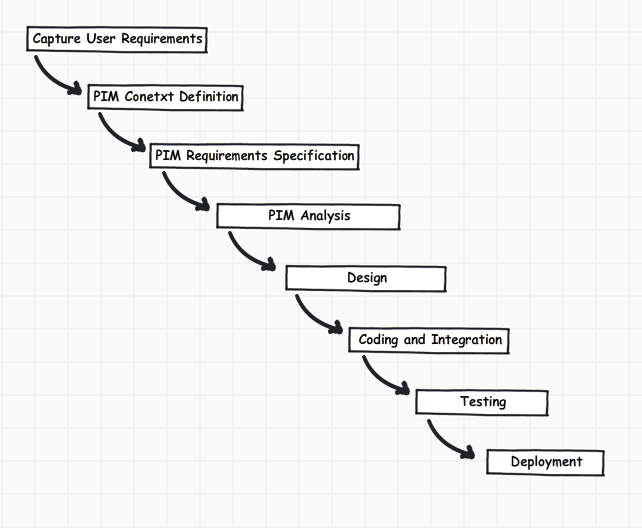
\includegraphics[width=0.9\textwidth]{figure/fig_MDDProcess.png}
			\newline
			\textbf{Fuente:} Elaboraci\'on propia basada en \textit{The MDD
			Process}, visto por Frattini y Silva en \cite{Frattini2007}, p\'agina 75,
			Figura 19.
		\label{fig:MDDProcess}
	\end{figure}
	 
	En la Figura \ref{fig:MDDProcess} se muestran las etapas del proceso de
	\ac{MDD} desde la etapa de captura de requerimientos
	hasta la etapa de liberaci\'on. Como se puede notar en la segunda etapa del
	proceso se realiza la definici\'on del contexto del \ac{PIM} etapa en la cual se
	define el proceso de negocio en el cual la abstracci\'on ser\'a modelada, as\'i como
	tambi\'en en la etapa de dise\~no se realiza los preparativos para el desarrollo
	del \ac{PDM} en la etapa de codificaci\'on e integraci\'on.
	
	\section{Web Modeling Language}
	\label{sec:WebML}
%	El lenguaje est\'a orientado a proporcionar una especificaci\'on de alto nivel de%
%	aplicaciones web, las cuales pueden ser traducidas en c\'odigo ejecutable por
%	medio de un \ac{CASE}, 
	
	
	Bongio et al. en \cite{Ceri2000} comenta que \ac{WebML} est\'a basado en
	otras propuestas de lenguajes de dise\~no web como por ejemplo:
	
	\begin{itemize}
	  \item HDM: Pionero en \ac{MDD} de aplicaciones hipermedia (HDM-lite, HDM,
	  RMM, Strudel, OOHDM) cuyos lenguajes construyen constructores
	  navegacionales, a diferencia de \ac{WebML} este no incluye composici\'on
	  ortogonal y primitivas de navegaci\'on.
	  \item Araneus: Propuesta de dise\~no web e ingenier\'ia inversa
	  en la que la informaci\'on se describ\'ia por medio de un \ac{ERM} y el
	  modelo de navegaci\'on se realizaba mediante un \ac{NCM}.
	  Araneus pose\'ia un ciclo de vida el cual estaba compuesto por: un modelado
	  conceptual, un dise\~no l\'ogico y un \ac{ADM} para los
	  aspectos de navegaci\'on.
	  Pose\'ia primitivas predefinidas de navegaci\'on pero no modelaba la
	  presentaci\'on a un nivel abstracto.
	  \item OOHDM: El cual dirigi\'o las t\'ecnicas de modelado conceptual de
	  \ac{WebML}, era una metodolog\'ia para dise\~no de hipertexto que comparte
	  junto a \ac{WebML} la visi\'on de dimensiones ortogonales.
	  \item \ac{UML}: Ha servido de base para muchas metodolog\'ias incluso para
	  dise\~no web, un ejemplo de ello puede ser visto en el trabajo realizado por
	  Fraternalli et al. en \cite{Moreno2006} en el cual mediante una extensi\'on
	  de \ac{UML} se logra modelar como si de \ac{WebML} se tratase, esto se
	  realiza mediante la utilizaci\'on de diagramas de clases, los cuales son
	  mejor descritos por Fowler en \cite{Fowler2003}.
	\end{itemize}
	 
	Bongio et al. en \cite{Ceri2000} comenta que las herramientas que antes exist\'ian, entre
	ellas las antes nombradas, ofrec\'ian poco apoyo para acortar la brecha entre la
	recolecci\'on de requerimientos y las fases sub--siguientes del proceso de
	desarrollo de aplicaciones web, es por esta raz\'on que el Proyecto \ac{W3I3} 
	(fundado por la Comunidad Europea bajo el Fourth Framework Program) se enfoc\'o
	en ``Intelligent Information Infrastructure'' para ``data intensive web
	application'', el proyecto fue dirigido por Otto Versand (e-commerce) y
	PTT(KPN) (web hosting service) los cuales produjeron un lenguaje de modelado
	web llamado \ac{WebML} y un \ac{CASE} que lo soporte, llamado Toriisoft.
	\ac{WebML} estaba dise\~nado para ser un lenguaje de alto nivel que pudiera
	cumplir con cubrir especificaciones independientes de la plataforma de data
	intensive web application, una personalizaci\'on one--to--one, acceso a
	m\'ultiples dispositivos y Toriisoft pod\'ia cumplir con estos aspectos
	adem\'as de cubrir el ciclo de vida entero y siguiendo un enfoque dirigido por
	modelos para dise\~no web centrado en el uso de \ac{WebML} ya que como comenta
	Lowe y Tongrungrojana en \cite{Lowe2003} los enfoques de modelado web eran
	raramente dirigidos a las conexiones entre aspectos de dise\~no detallado y la
	amplia informaci\'on del ambiente, particularmente en t\'erminos del flujo de
	informaci\'on entre el sistema, la organizaci\'on y entidades externas, lo cual
	si se lograba con un dise\~no dirigido por modelos.

	A lo anteriormente explicado Nugraha en \cite{Nugraha2007} y
	Ceri et al. en \cite{Matera2003} comentan que \ac{WebML} es un \ac{DSL}, el
	cual describe la composici\'on, navegaci\'on, contenido, organizaci\'on y representaci\'on en un
	hipertexto, todo ello para especificar la estructura del contenido de una
	aplicaci\'on web mientras que Bongio et al. en \cite{Ceri2000} dice que \ac{WebML} es una
	notaci\'on para especificar p\'aginas web complejos en un nivel conceptual y capaz de
	describir a alto nivel una p\'agina web bajo distintas dimensiones ortogonales
	como lo hacia HDM y OOHDM, como por ejemplo:
	
	\begin{itemize}
	  \item Su contenido (modelo estructural)
	  \item Las p\'aginas que lo componen (modelo de composici\'on)
	  \item La topolog\'ia de sus links entre p\'aginas (modelo de navegaci\'on)
	  \item Requerimientos gr\'aficos
	  \item Las capas para renderizaci\'on de p\'aginas (modelo de presentaci\'on)
	  \item Las caracter\'isticas de personalizaci\'on para el contenido de entrega
	  one--to--one (modelo de personalizaci\'on).
	\end{itemize}
	
	Brambilla et al. en \cite{Brambilla2010} comenta tambi\'en que \ac{WebML} es
	una metodolog\'ia de un alto nivel de notaci\'on para datos, servicios y procesos centrados en el desarrollo
	de aplicaciones web. Ya que este permite especificar el modelo de datos de una
	aplicaci\'on web y uno o m\'as modelos de hipertexto que puede ser basado en
	especificaci\'on de procesos de negocio y que puede explotar la invocaci\'on de
	servicios web, personalizar la l\'ogica del back--end y las interfaces web
	enriquecidas.

	\begin{figure}[here]
    	\centering
    	\caption{Ciclo de Vida de Software en WebML}
    	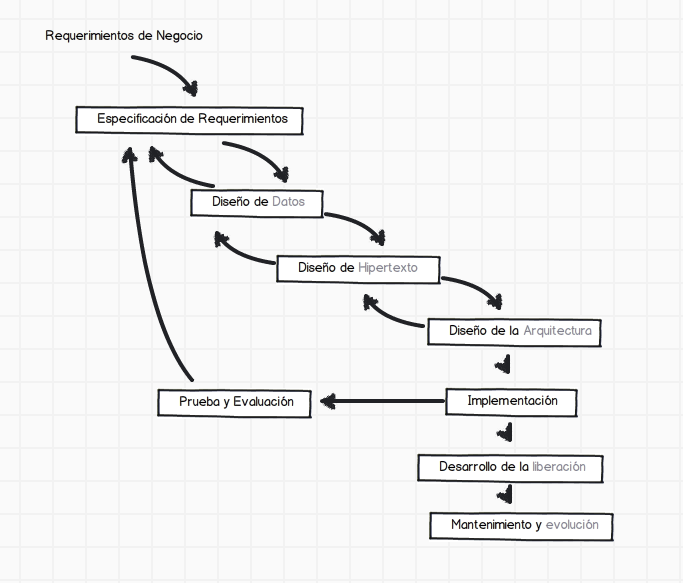
\includegraphics[width=0.9\textwidth]{figure/fig_WebMLLifeCicle.PNG}
		\newline
			\textbf{Fuente:} Elaboraci\'on propia basada en \textit{The extended WebML
			process}, visto por Frattini y Silva en \cite{Frattini2007}, p\'agina 81,
			Figura 24.
		\label{fig:WebML_LifeCicle}
    \end{figure}
	
%Consultar si es correcto requisitos o requerimientos
	Como se muestra en la Figura \ref{fig:WebML_LifeCicle} el enfoque de \ac{WebML}
	esta dividido en diferentes fases, Bongio et al. en \cite{Ceri2003} nos comenta
	que el dise\~no fue inspirado en la espiral de Boehm, proceso el cual debe de ser aplicado de
	una manera iterativa e incremental en la cual varias fases son repetidas y
	refinadas hasta que los resultados cumplan con los requisitos de la aplicaci\'on.
	
	A pesar de que podemos notar varias fases, se puede diferenciar
	un total de $3$ estados principales cuando se modela y/o trabaja con
	\ac{WebML}, las cuales Brambilla et al. en \cite{Brambilla2010} denomina como
	las etapas m\'as importantes del proceso de desarrollo, las cuales son las
	etapas de Dise\~no de datos, Dise\~no de hipertexto y el Dise\~no de la
	Arquitectura ya que el lenguaje est\'a orientado a proporcionar una
	especificaci\'on de alto nivel de aplicaciones web.\\\newline
	
	\fbox{\parbox[b]{\linewidth}{\textbf{\underline{\emph{Nota:}}} Haciendo un
	par\'entesis. Brambilla et al. en \cite{Brambilla2010} comenta tambi\'en que
	estas aplicaciones web pueden ser traducidas en c\'odigo ejecutable, como se
	comento anteriormente por medio de un \ac{CASE}, como Toriisoft por
	ejemplo, la cual debe de proveer algunas propiedades como son: 
	
	\begin{itemize}
	  \item Una representaci\'on visual que transmita las caracter\'isticas esenciales
	  de sus primitivas lo que puede ser visualizado en diagramas, pudiendo sus
	  conceptos ser representados mediante un \ac{ERM} y/o \ac{UML}.
	  \item Estar provisto de una representaci\'on textual basada en \ac{XML}.
	\end{itemize}
	
	Un \ac{CASE} con estas caracter\'isticas Acerbis et al. en \cite{Acerbis2007}
	comenta que es m\'as f\'acil el dominar la complejidad del desarrollo de aplicaciones web.}}
	\\\newline
	
	Dentro de las etapas nombradas anteriormente (Dise\~no de Datos, de
	Hipertexto y de Arquitectura) se pueden diferenciar estados muy importantes y
	que se ven durante la mayor parte del desarrollo de aplicaciones basadas en web
	mediante \ac{WebML} los cuales Bongio et al. en \cite{Ceri2000} nombra como dimensiones
	ortogonales o como Ceri et al. en \cite{Matera2003} y Frattini y Silva en
	\cite{Frattini2007} lo identifican, con el nombre de Modelado Conceptual y estos son:
	
	\begin{itemize}
	  \item \ac{WebML} Data Model o Structural Model - Est\'a
	  estrechamente ligado a la etapa ``Dise\~no de Datos'' en la cual se modela
	  mediante diagramas \ac{ERM} y/o \ac{UML} de clases primitivos con un valor a\~nadido de
	  relaciones (llamadas derivadas) en las cuales se utiliza un lenguaje
	  declarativo (como \ac{OQL} y/o \ac{OCL}, en este contexto es mayormente usado
	  el modelado mediante \ac{ERM} en la cual las entidades son definidas como
	  contenedores de elementos de datos y las relaciones definidas como conexiones
	  sem\'anticas entre entidades. Las entidades tienen propiedades nombradas,
	  llamadas atributos y tipos asociados como lo nombra Ceri et al. en
	  \cite{Matera2003}.
	  Las entidades pueden ser organizadas en generalizaciones jer\'arquicas y las
	  relaciones pueden ser restringidas por medio de cardinalidad limitada. En
	  esta fase se puede nombrar algunas actividades importantes.		  

	  \begin{itemize}
	    \item Modelado de grupos - En la cual se modela los requerimientos de
	    grupos de usuarios en entidades y relaciones.
	    \item Identificaci\'on de sincronizaci\'on de objetos - Similar al ciclo de
	    vida del productor--consumidor en la cual se ve como los actores
	    trabajan con cada objeto y su interacci\'on con estos.
	    \item Identificaci\'on de objetos compartidos - Aqu\'i se observa que
	    fase son utilizados que objetos.
  	  \end{itemize}
  	  
  	  Bongio et al. en \cite{Ceri2000} enfatiza este modelo a las entidades, las cuales como se
  	  comenta: \textit{son la base de las relaciones sem\'anticas}.

	  \item WebML Hypertext Model - Est\'a estrechamente ligado a la
	  etapa de ``Dise\~no de hipertexto'' en la cual se modela las interfaces de
	  Front--End de la aplicaci\'on web y en la cual se realiza una organizaci\'on
	  interna en t\'erminos de componentes, o tambi\'en llamados en \ac{WebML}
	  \textit{Content Units} o \textit{Unidades de contenido}.
	  Es aqu\'i donde se inicia el dise\~no propiamente dicho y en donde se producen
	  esquemas de site views en el \textit{top} del esquema de datos previamente modelado,
	  es aqu\'i donde se utilizan elementos de contenido como son:
	  
%%%%%%%%%%%%%%%%  Modificaciones a ralizar.	  
	  \begin{itemize}
		\item Site Views - Es el producto del modelado espec\'ifico para un conjunto
		de requerimientos, el cual consiste en el conjunto de las \textit{\'areas}
		las cuales son las principales secciones del hipertexto y comprende
		recursivamente otras \textit{sub--\'areas} o \textit{p\'aginas} que se
		encuentran en uno de los varios contenedores de informaci\'on entregados por
		el usuario.
		\item Content Units - Este representa una abstracci\'on de un objeto el cual
		ser\'a publicado en la aplicaci\'on web. Habiendo varios tipos del mismo, como por
		ejemplo:
			  
		  \begin{itemize}
		    \item Data Unit - Existe en una relaci\'on $1 \to 1$, entre un atributo y
		    una instancia de entidad.
		    \item Multi--data unit - Existe en una relaci\'on de $n \to n$, entre
		    atributos e instancias de entidades.
		    \item Index unit - Existe en una
		    relaci\'on $ n \to 1$, entre una lista de atributos a una instancia de
		    entidad (la cual se le considera como: una selecci\'on)
		    \item Scroller Unit - Se utiliza para realizar una b\'usqueda en un
		    conjunto ordenado de objetos
		    \item Entry Unit - Su funci\'on principal es la de implementar
		    formularios y poder servir de interfaz para los content units anteriores.
		  \end{itemize}
			  
%			  \begin{figure}[here]
%				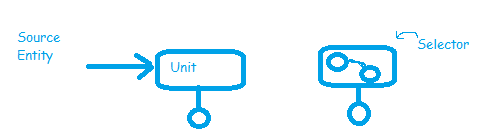
\includegraphics[width=0.9\textwidth]{figure/fig_ContentUnit.png}
%				\caption{Content Units}
%				\label{fig:ContentUnits}
%			  \end{figure}

		\item Pages - Llamadas tambi\'en sub--\'areas, las cuales ser\'an el
		contenedor de los Content Units y ser\'an los que se muestren como parte
		l\'ogica al desarrollador y parte visual al usuario final, estas pueden ser de diferentes
		tipos:

		  \begin{itemize}
		    \item Home Page
		    \item Default
		    \item Landmark - Estas se dividen por tipo de enlace, entre ellas como:
		    Link/Unit y Link/Pages, llamados com\'unmente links contextuales y no
		    contextuales respectivamente.
		  \end{itemize}
	  \end{itemize}
			
        \begin{figure}[here]
        	\centering
        	\caption{Modelado en WebML}
			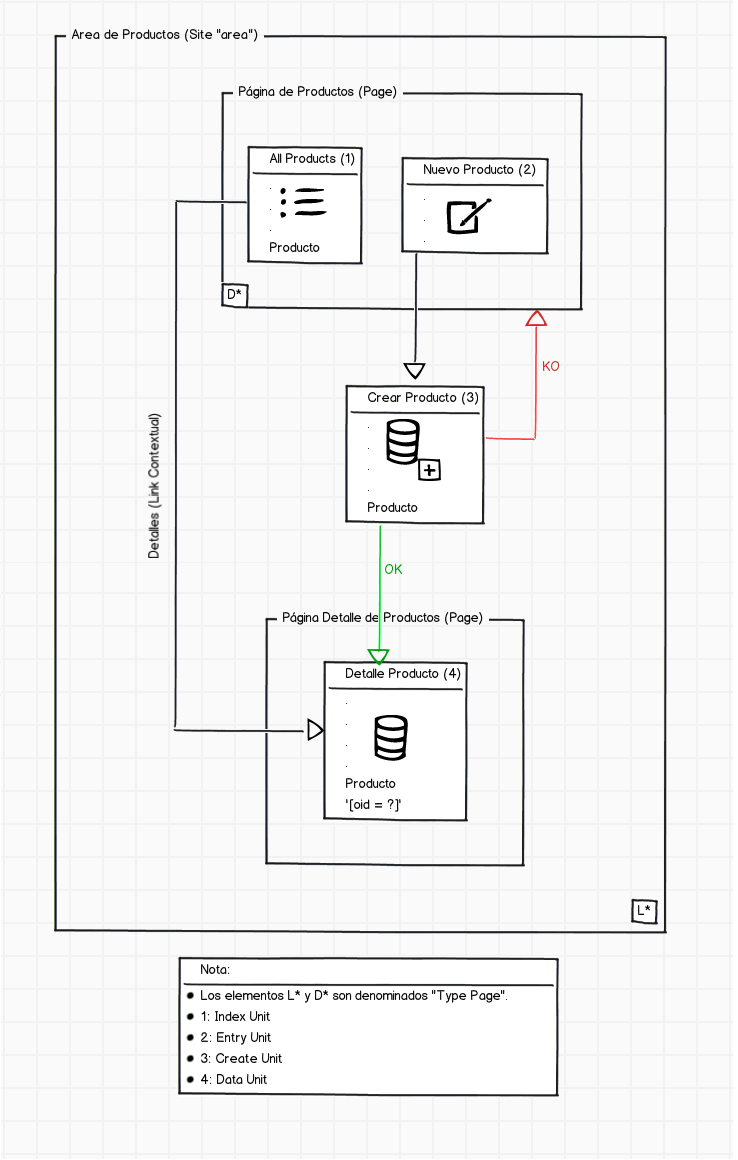
\includegraphics[width=0.9\textwidth]{figure/fig_ModelingWebML.png}
			\newline
			\textbf{Fuente:} Elaboraci\'on propia de elementos de modelado de hipertexto
			para WebML.	
			\label{fig:ModelingWebML} 
        \end{figure}
        
        En la Figura \ref{fig:ModelingWebML} se muestra un ejemplo en el cual
        podemos ver todos los elementos comentados anteriormente, as\'i como
        algunos de tipo behavioral (de comportamiento), se tiene que tener
        especial cuidado en los tipos de link: Link/Unit y Link/Pages
        (contextuales y no contextuales respectivamente), ya que de ellos
        depender\'a la navegabilidad de la aplicaci\'on, para este ejemplo se
        presentan ambos tipos:
        \begin{itemize}
          \item Links contextuales: \textit{Detalle} y \textit{OK}, los cuales
          como se puede ver, el $1^o$ navega, desde un Index Unit hasta un Data
          Unit y el $2^o$ desde un Create Unit hasta un Data Unit (al link se le
          coloc\'o \textbf{OK}, ya que se seguira ese flujo si es que la
          operaci\'on de guardado de esta unidad era exitoso).
          \item Link no contextual:\textit{KO}, el cual seg\'un la l\'ogica del
          Create Unit, si es que la operaci\'on de guardado es fallida, entonces
          esta seguira un flujo hacia un p\'agina (generalmente marcada como
          p\'agina de error).
        \end{itemize}
		
		Habiendo visto la mayor parte de los elementos de los que consta el Modelo
		de Hipertexto Web, siendo su unidad b\'asica: la unidad de
		contenido cabe nombrar que Davies y Mintz en \cite{Davies2009} lo denotan con
		el nombre de Unit Types, en el cual su comportamiento
		tomando una postura orientada a objetos y comentando que estos debieran tener
		un comportamiento polim\'orfico, en otras palabras deber\'ian tener varios
		comportamientos o disponibilidades para los usuarios. Pero a este comentario
		tambi\'en se dio una contraparte, en la cual se dice que el cliente/servidor
		puede romper el polimorfismo para aplicaciones web sociales, entre los aspectos
		m\'as importantes el causante puede ser que el navegador no sea compatible con
		estas unidades, es por ello que propone algunos puntos para que los Unit Types
		conserven su aspecto polim\'orfico, como son:
		
		\begin{itemize}
		  \item El comportamiento de las unidades debe de ser extensible y deben
		  poseer la capacidad de  poder modificarse.
		  \item Los contenedores o tags\footnote{Los tag o etiquetas son un tipo de
		  metadatos, pues proporcionan informaci\'on que describe una determinada
		  unidad de informaci\'on.} deben ser referenciales es por ello que se
		  hace una relaci\'on $1 \to 1$ entre puntero e instrucciones por objeto o archivo.
		  \item El Type Structure\footnote{Los type structure representa las
		  relaciones entre los unit types.} debe ser ``jer\'arquicamente heredado'' en
		  otras palabras, el contenido debe de ser heredado por cada tag.
		  \item Las relaciones deben de ser \'integramente inicializables \'osea que las
		  relaciones entre unidades de contenido como hiperv\'inculos tradicionales
		  sean links de unidad a unidad, lo que vendr\'ian a ser relaciones.
%aqu\'i va el nombre para las unidades de tipo operacional
		  \item En aplicaciones sociales basadas en web se definen como relaciones
		  entre unidades y unidades externas\footnote{En el contexto de la web social
		  estas unidades externas toman el comportamiento de componentes (o mash up's)
		  o aplicaciones externas, como por ejemplo las conexiones con
		  componentes de Facebook o componentes de Google hacia otras aplicaciones.}.
		  \item Se debe buscar que el control de acceso sea de tipo fluid--granular
		  donde:
		  
		  	\begin{itemize}
		  	  \item Fluidez o fluidity: Existencia de distinci\'on marcada entre un
		  	  usuario y un administrador de la aplicaci\'on.
		  	  \item Granularidad o granularity: Control sobre cada campo de la unidad.
		  	\end{itemize}
		  	
		  \item El direccionamiento debe ser independiente del dominio, por ejemplo:
		  si se mueve el contenido todo deber\'ia de funcionar igual.
		  \item En el momento de la construcci\'on debe existir alg\'un
		  tipo de versionamiento comprensible.
		  \item Si se desarrolla alg\'un componente que utilice m\'etodos de borrado,
		  estos deben de ser controlados por el usuario (existencia de un borrado
		  verdadero de los archivos propios\footnote{Cuando se habla sobre
		  borrado o eliminaci\'on de un registro en base de datos se habla
		  sobre 2 tipos de borrado; uno l\'ogico y uno f\'isico, el primero
		  solo elimina el registro dependiendo de una l\'ogica de
		  visualizaci\'on a diferencia del segundo que elimina el registro desde la
		  misma base de datos.})
		  \item Al momento de la construcci\'on se debe considerar que las licencias de
		  software deben ser free/open source: para poder inspeccionar y modificar el
		  c\'odigo.
		\end{itemize}
		
		Bongio et al. en \cite{Ceri2000} definen esta dimensi\'on como un conjunto de
		hipertextos para la p\'agina web en el cual cada hipertexto define un siteview y cada siteview est\'a
		compuesto por sub--modelos, los cuales representan la fase de
		``Dise\~no de la Arquitectura'' en la cual se realiza el modelado de la
		apariencia gr\'afica y los estilos a ser utilizados en la aplicaci\'on web
		respectivamente, y estos son:
		
		\begin{itemize}
		  \item [a.] Modelo de Presentaci\'on - Representa la interfaz gr\'afica o
		  \textit{look and feel} de las p\'aginas identificadas en el modelo de
		  composici\'on la cual el usuario final vera cuando acceda a la aplicaci\'on, independiente de
		  la informaci\'on ha ser mostrada. Estas en \ac{WebML} son renderizadas
		  mediante hojas de estilo.
		  \item [b.] Modelo de Personalizaci\'on - Que representa la variaci\'on de
		  estilos que tendr\'a la aplicaci\'on en su parte gr\'afica. Este sub--modelo
		  va enlazado con las entidades llamadas \textbf{User} y \textbf{Group} en las
		  cuales se puede definir reglas de negocio espec\'ificas para usuarios y grupos a los que estos
		  pertenecen (puede ser hecho con \ac{OQL}).
		  \item [c.] Modelo de Composici\'on - En la cual se especifica que
		  unidad de contenido pertenece a la p\'agina y que p\'agina
		  pertenece a que hipertexto.
		  \item [d.] Modelo de Navegaci\'on - Expresa como es que las unidades
		  de contenido y las p\'aginas ser\'an enlazadas en el hipertexto
		  mediante links (o enlaces) los cuales se dividen en:
		  
		  \begin{itemize}
		    \item Enlaces contextuales: Conecta unidades dependiendo de una sem\'antica
		    expresada por el esquema de la aplicaci\'on. Un enlace contextual acarrea
		    informaci\'on (llamado contexto), sint\'acticamente se denota por un elemento
		    ``INFOLINK''.
		    \item Enlaces no contextuales: Conecta p\'aginas que sean independientes
		    de las unidades que ellos contengan, sint\'acticamente se denota por un elemento
		    ``HYPERLINK''.
		  \end{itemize}  
		  
		\end{itemize}
		
		Adem\'as de los enlaces, un Modelo de Navegaci\'on debe
		cumplir con poseer una l\'ogica de hipertexto valida, \'osea que se cumplan
		las siguientes reglas:
		 
		\begin{itemize}
		  \item Accesibilidad o reachability: No debe haber p\'aginas sin alg\'un tipo
		  de enlace (posiblemente el homepage rompe esta regla).
		  \item Flujo de contexto: Si alguna unidad de contenido necesita en alg\'un
		  momento de su ciclo de vida de informaci\'on contextual esta debe ser dada por
		  un link contextual desde otra(s) unidad(es) o p\'agina(s).
		  \item Unicidad de contexto: Si no existe o si hay m\'as de una forma de
		  recibir contexto,  solo una debe de ser habilitada y las dem\'as
		  des--habilitadas.
		\end{itemize}
		
		Bongio et al. en \cite{Ceri2000} nos habla de la existencia de $3$ actores
		principales en todo el proceso de dise\~no de \ac{WebML}:
		
		\begin{itemize}
		  \item Un experto de datos el cual dise\~na el ``structural model''.
		  \item Un arquitecto de aplicaciones el cual dise\~na p\'aginas y la navegaci\'on
		  entre ellas.
		  \item Un arquitecto de estilos el cual dise\~na los estilos de presentaci\'on de
		  las p\'aginas.
		\end{itemize}
		
		Adicionalmente a estos $3$ actores de dise\~no tambi\'en es necesario un actor
		administrador de la p\'agina web, quien dise\~na las opciones de usuario y
		personalizaci\'on, incluyendo las reglas de negocio.
		
		Estos actores participar\'an en el proceso de dise\~no de \ac{WebML} de forma
		iterativa y como comenta Ceri et al. en \cite{Matera2003} y Frattini y Silva
		en \cite{Frattini2007} se realiza las siguientes etapas.
		
		\begin{itemize}
		  \item Especificaci\'on y/o an\'alisis de Requerimientos (tambi\'en llamada
		  Requirement Collection): Es la etapa en la cual se recolecta informaci\'on
		  acerca del dominio de la aplicaci\'on, funciones esperadas, limitaciones y se
		  le espec\'ifica a trav\'es de descripciones f\'aciles de entender.
			\begin{itemize}
			  \item INPUT - Requerimientos de negocio
			  \item OUTPUT - Identificaci\'on de grupos de usuario, especificaci\'on de
			  requerimientos funcionales, identificaci\'on de objetos de informaci\'on CORE y
			  descomposici\'on de la aplicaci\'on web en site views.
			  \item Adicionalmente se observa que es necesario el uso de determinados
			  diagramas \ac{UML}, tales como:
	
			  \begin{itemize}
			    \item Diagrama de actividades - Para poder modelar los escenarios
			    y actividades as\'incronas
			    \item Diagrama de casos de uso - En la cual se realiza una variante
			    determinada y se utiliza \'arbol jer\'arquico de usuarios, en el cual se
			    puede describir los niveles de acceso de los mismos hacia y/o desde la
			    aplicaci\'on web.
			    \end{itemize}
	
			\end{itemize}
		  
		  \item Data Design: Se dise\~na el Structural Model y si ya existieran
		  esquemas legados se hace ingenier\'ia reversa.
		  \item Hypertext Design ``in the large'': Se identifican p\'aginas y unidades,
		  enlaz\'andolos, en pocas palabras se define el ``esqueleto'' del site view las
		  cuales se mejorar\'an iterativamente. (Para esta etapa las herramientas
		  basadas en Web deben soportar el r\'apido prototipado y
		  retro--alimentaci\'on).
		  \item Hypertext Design ``in the small'': En esta segunda etapa de dise\~no de
		  hipertexto se enfocan en tratar cada p\'agina y unidad individualmente.
		  Durante el dise\~no de la p\'agina el arquitecto de la aplicaci\'on web puede
		  descubrir que una p\'agina requiere informaci\'on adicional o alg\'un cambio de
		  conceptos sem\'anticos.
		  \item Presentation Design: Se dise\~na el estilo para las p\'aginas cuando ya
		  estas son lo suficientemente estables.
		  \item User and Group Design: El administrador define las caracter\'isticas de
		  los perfiles de usuarios basados en requerimientos de personalizaci\'on.
%******* aqu\'i comienza desde el inicio en una nueva iteraci\'on *******
		  \item Customization Design: Se realiza la personalizaci\'on de la p\'agina
		  web mediante reglas de negocio.
			
		\end{itemize}

	\end{itemize}
	
%Secci\'on para la explicaci\'on de RUP3C	
	\section{Trabajos Relacionados}
	\label{sec:RelatedWorks}	
		\subsection{RUP3C}
		\label{ssec:RUP3C}
		RUP3C fue desarrollado para poder resolver la falencia de una metodolog\'ia para
		el desarrollo de aplicaciones groupware. Esta metodolog\'ia se desarroll\'o en base
		a $3$ aspectos:
		
		\begin{enumerate}
		  \item Office Automation
		  \item Hipertexto
		  \item Enfoque grupal 
		\end{enumerate}
		
		Dentro de estos $3$ aspectos actualmente podemos notar que el punto $1$ y $2$
		poseen al menos una forma de desarrollo de aplicaciones como Gerosa et al. en
		\cite{Gerosa2005} comenta, pero en lo referente a desarrollo de aplicaciones groupware era
		casi imposible y aun inclusive hoy en d\'ia se requiere de programadores
		calificados, ya que se carec\'ia de una gu\'ia para desarrollar aplicaciones
		mientras se generaban artefactos relacionados. Estas fueron algunas de las razones para
		el desarrollo del modelo RUP3C el cual Gerosa et al. en \cite{Gerosa2005}
		comenta que su nombre proviene de una extensi\'on de la metodolog\'ia \ac{RUP}
		a la cual se le incremento el enfoque de desarrollo groupware bas\'andose en $3$ puntos, los
		cuales son:
		
		\begin{itemize}
		  \item Comunicaci\'on: Ya que se basa en un intercambio de mensajes y
		  negociaci\'on de compromisos.
		  \item Coordinaci\'on: Es la administraci\'on de recursos para resolver conflictos
		  y de esta manera facilitar la cooperaci\'on.
		  \item Cooperaci\'on: Esta es la producci\'on conjunta de miembros de un grupo
		  dentro de un espacio compartido (para completar tareas).
		\end{itemize}
		
		Aspectos b\'asicos del dise\~no: Asociaci\'on
		
		\begin{itemize}
		  \item Administrador de versiones
		  \item Registro de accesos
		  \item An\'alisis est\'atico
		  \item Sistema de recomendaci\'on
		  \item Mecanismo de b\'usqueda y ranking 
		\end{itemize}
		
		
	    \begin{figure}[here]
	    	\centering
	    	\caption{Modelo: RUP3C}
	    	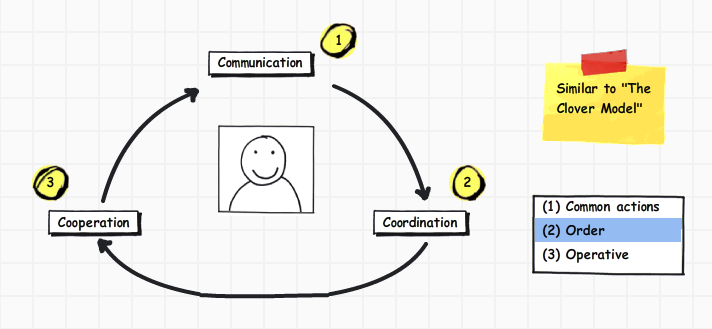
\includegraphics[width=0.9\textwidth]{figure/fig_rup3cModel.png}
			\newline
			\textbf{Fuente:} Elaboraci\'on propia basada en \textit{Diagram of the 3C
			collaboration model} de Gerosa et al. en \cite{Gerosa2005}, p\'agina 5,
			Figura 1.
			\label{fig:RUP3CModel}
	    \end{figure}
		
		
		Algo que Gerosa et al. en \cite{Gerosa2005} comenta es que es muy importante seguir la
		filosof\'ia de ``un problema por versi\'on'', es por ello que se puede notar en la
		Figura \ref{fig:RUP3CModel} cada uno de los $3$ puntos base de esta
		metodolog\'ia posee una parte del ciclo de interacci\'on con el usuario as\'i como
		consigo mismas\footnote{Adem\'as de ser una extensi\'on de la metodolog\'ia
		\ac{RUP} tambi\'en lo es del cl\'asico modelo en tr\'ebol y de la misma forma
		extendido de la forma en que con esta metodolog\'ia se pueda soportar el
		desarrollo de aplicaciones groupware.}.
		
\chapter{PROPUESTA}		   		
\label{chap:Proposal}
	En este cap\'itulo se presenta el desarrollo de la propuesta de este trabajo
	dividida en $3$ secciones de la siguiente manera:
	
	\begin{enumerate}
	  \item \textbf{Comunicaci\'on:} En esta secci\'on se brinda una descripci\'on
	  de como se realizar\'a la captura de requerimientos o espec\'ificamente  en como
	  este modelo desarrollar\'a la primera parte del ciclo de vida de esta
	  propuesta.
	  %\item \textbf{Planeaci\'on:} Para esta secci\'on se dara una breve rese\~na
	  %de como se realizara la planeaci\'on o divisi\'on de tiempo en el desarrollo
	  %de un proyecto.
	  \item \textbf{Modelado:} En esta secci\'on se muestra el panorama de
	  \textit{an\'alisis} y \textit{dise\~no} de esta propuesta.
	  \item \textbf{Construcci\'on:} Para esta secci\'on se mostrar\'a la
	  construcci\'on de las custom units necesarias para el desarrollo de una
	  aplicaci\'on social\footnote{Para este cap\'itulo y secci\'on se
	  presentar\'a el desarrollo de nuestra propuesta, para
	  el siguiente cap\'itulo es donde se presentara un caso de estudio con la
	  utilizaci\'on de cada una de estas etapas.}.
	  %\item \textbf{Despliegue:} Aunque esta etapa no se tomara para nuestra
	  %propuesta cabe mencionar que toda metodolog\'ia ha de tener siempre una etapa
	  %de \textit{Despliegue} o \textit{liberaci\'on} del producto.
	\end{enumerate}
	
	\section{Comunicaci\'on}
	\label{sec:communication}
	En esta secci\'on se presenta una propuesta de variaci\'on del ciclo
	de vida de la metodolog\'ia de desarrollo de software \ac{WebML}, para soportar
	el paradigma social.
	
%	\begin{figure}[here]
%    	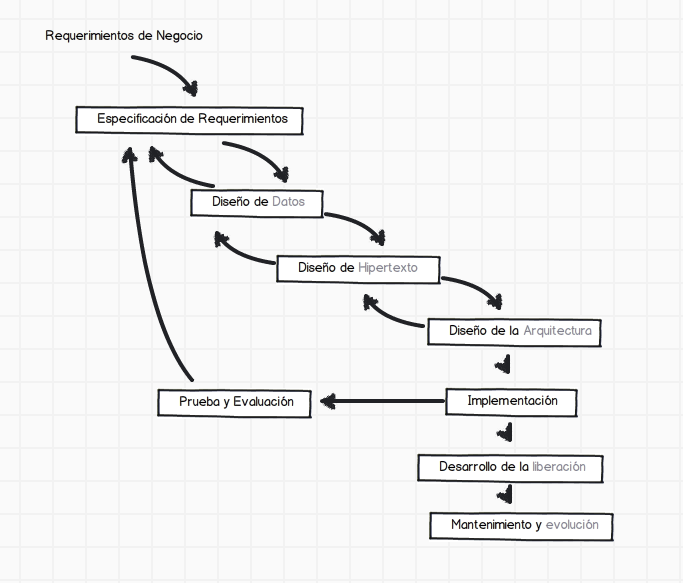
\includegraphics[width=0.9\textwidth]{figure/fig_WebMLLifeCicle.PNG}
%		\caption{Ciclo de Vida de Software en WebML}
%		\label{fig:WebML_LifeCicle}
%    \end{figure}
    
    \begin{figure}[here]
        \centering
    	\caption{Propuesta de Ciclo de Vida de Software en Social WebML}
    	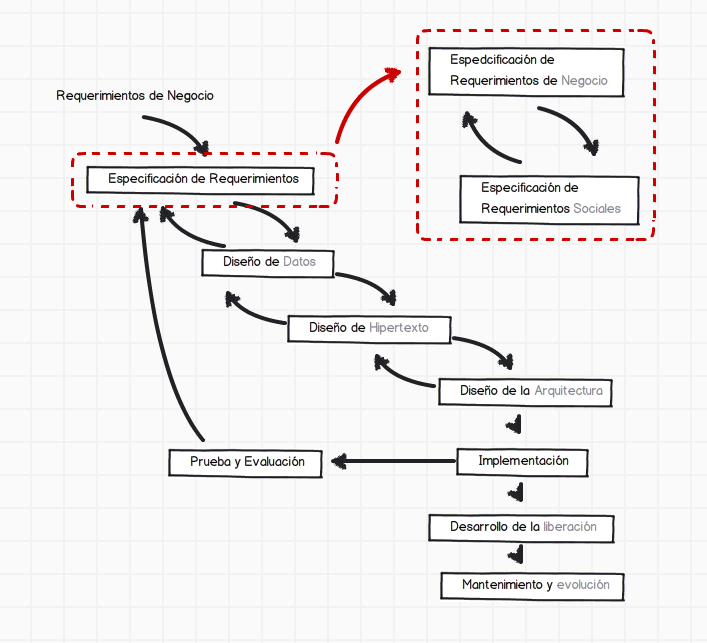
\includegraphics[width=0.9\textwidth]{figure/fig_SocialWebMLLifeCicle.PNG}
		\newline
			\textbf{Fuente:} Elaboraci\'on propia basada en \textit{The extended WebML
			process}, visto por Frattini y Silva en \cite{Frattini2007}, p\'agina 81,
			Figura 24.
		\label{fig:SocialWebML_LifeCicle}
    \end{figure}
    
	Como se observa en la Figura \ref{fig:WebML_LifeCicle} vista anteriormente
	cuando se describ\'ia los estados por los que el software desarrollado bajo la
	metodolog\'ia \ac{WebML} pasa. Se dar\'a hincapi\'e en la primera etapa, la
	\textit{Especificaci\'on de Requerimientos}, aquella que para esta secci\'on
	posee mayor relevancia y aquella que representa la propuesta inicial ya que es
	donde se realizar\'a la captura de requerimientos sociales, esto se ve reflejado en la Figura
	\ref{fig:SocialWebML_LifeCicle}, en la cual, enmarcada en l\'ineas punteadas
	rojas, se encuentra una nueva rama en el proceso o para ser mas espec\'ifico un
	desglose de una de las etapas en dos nuevas etapas, las cuales han
	sido etiquetadas como:

	\begin{enumerate}
	  \item \textbf{Especificaci\'on de Requerimientos de Negocio:} En esta etapa se
	  realizar\'a todas las acciones tradicionales de \textbf{captura de
	  requerimientos}, elicitaci\'on, ``especificaci\'on", educci\'on, etc., con
	  respecto al negocio del aplicativo por intermedio del stakeholder y/o
	  usuario, esto siguiendo las bases de \ac{UML} y \ac{WebML}.
	  \item \textbf{Especificaci\'on de Requerimientos Sociales:} En esta etapa
	  se presenta parte de la propuesta, la cual se realizar\'a una
	  \textbf{captura} de \textit{requerimientos sociales} o un conjunto de
	  \textit{necesidades sociales} inicialmente comprendidas como parte de un
	  conjunto de patrones sociales de dise\~no, los cuales se pueden ver en
	  la Tabla \ref{tab:socialPatternDesign} en la cual se presenta un resumen del
	  trabajo realizado por Frattini y Silva en \cite{Frattini2007} y por Bozzon en
	  \cite{Bozzon2009}, adicional de una referencia de cuales son los otros
	  patrones sociales de dise\~no con los que se relacionan los patrones sociales
	  de dise\~no nombrados en la Tabla \ref{tab:socialPatternDesign}.
	  
	  	\begin{table}[htbp]
	  	\caption{Patrones Sociales de Dise\~no}
	  	\centering
			\begin{tabular}{|c|l|l|}
			\hline
				\textbf{C\'odigo} & \textbf{Nombre} & \textbf{Patrones Relacionados}  \\
				\hline \multicolumn{3}{|c|}{\textbf{Front-End Patterns}} \\\hline
				\multicolumn{3}{|c|}{\textbf{Patrones Navegacionales}} \\\hline
				1 & Aggregation -- Mashup & 04, 20, 24 \\ \hline
				2 & Browse by connections & 14, 20 \\ \hline
				3 & Browse by tag -- Folksonomy & 06, 20 \\ \hline
				\multicolumn{3}{|c|}{\textbf{Patrones de Contribuci\'on}} \\ \hline
				4 & Exportation & 20, 21, 22, 25 \\ \hline
				5 & Flagging & 18, 20, 22 \\ \hline
				6 & Organization -- Grouping -- Tagging & 03, 18, 20, 21, 23, 24 \\ \hline
				7 & Publication & 06, 19, 21, 23, 24 \\ \hline
				8 & Rating & 17, 20, 23 \\ \hline
				9 & Recommendation -- Suggestion & 12, 19, 20, 23 \\ \hline
				\multicolumn{3}{|c|}{\textbf{Patrones Sociales}} \\ \hline
				10 & Group creation & 19, 20 \\ \hline
				11 & Group participation & 12, 13, 18, 20, 22 \\ \hline
				12 & Invitation & 18, 19, 23 \\ \hline
				13 & Permission setting & 20 \\ \hline
				14 & Relationship setting & 17, 20, 22 \\ \hline
				15 & Social visualization & 17, 22, 23 \\ \hline
				16 & Talk & 18, 20 \\ \hline
				\multicolumn{3}{|c|}{\textbf{Back-End Patterns}} \\ \hline
				17 & Evaluation & 21, 22 \\ \hline
				18 & Notification & 09, 12, 14, 16 \\ \hline
				19 & Payment & 23 \\ \hline
				20 & Permission check & 13 \\ \hline
				21 & Relevance adjustment & 17, 22 \\ \hline
				22 & Reputation adjustment & 17 \\ \hline
				23 & Reward & 17, 22 \\ \hline
				24 & Syndication & 06, 07 \\ \hline
				25 & Importation &  \\ \hline
			\end{tabular}
			\newline
			\textbf{Fuente:} Elaboraci\'on propia basada en el trabajo de Frattini y
			Silva en \cite{Frattini2007}, Cap\'itulo: Patterns (p\'agina 24) e
			Implementation (p\'agina 112).
			\label{tab:socialPatternDesign}
		\end{table}
	
	  De los patrones sociales de dise\~no mostrados, aquellos los cuales son
	  m\'as relevantes para este trabajo son:
	  
	  \begin{itemize}
	    \item \textbf{Aggregation: } tambi\'en conocido como \textit{MashUp} en donde
	    la actividad mas importante es la de poder empotrar ``servicios'' de otros
	    proveedores dentro de una aplicaci\'on, pudiendo ser: juegos, canales
	    IRC, widgets, etc.
	    \item \textbf{Publication: } La actividad m\'as importante es la de
	    compartir contenido (comentarios, fotos, videos, etc.) a otros individuos, asociados
	    de una determinada forma al individuo que lo ``public\'o''.
	    \item \textbf{Organization: } tambi\'en conocido como \textit{Grouping} o
	    \textit{Tagging}; mediante la cual se podr\'a hacer una ``referencia'' a
	    otros individuos o contenido creado por los mismos.
	  \end{itemize}
	  
	  En la Figura \ref{fig:SocialFlowDiagram} se puede ver un Diagrama de Flujo
	  del comportamiento b\'asico de un individuo, seg\'un esta propuesta, para
	  ello se tienen que explicar algunos t\'erminos, importantes que dar\'an
	  m\'as sentido a la figura anterior.
	  
	  	\begin{itemize}
			\item \textbf{\ac{FOAF}}:\footnote{Para este contexto se tomar\'a en cuenta
			uno de los primeros comentarios en este trabajo, acerca de los estudios
			realizados acerca de los grados de separaci\'on entre dos personas} Este
			t\'ermino, m\'as usado en Web Sem\'antica, se usa para describir los grados de
			separaci\'on entre $2$ individuos, su uso m\'as allegado a la web sem\'antica,
			sin salir del contexto es mejor explicado por Brambilla y Facca en
			\cite{Brambilla2007} donde se busca modelar la Web Sem\'antica basado en la
			metodolog\'ia \ac{WebML} siendo uno de los principales conceptos: \ac{FOAF},
			este aspecto es utilizado para la mayor\'ia de las caracter\'isticas que
			sirvieron para comparar \ac{WebML} con otras, en donde esta metodolog\'ia
			a\~nadida al concepto sem\'antico result\'o en poseer o soportar todas las
			caracter\'isticas relevantes total o parcialmente.
			\item \textbf{Compartir Informaci\'on:} Representa una de las acciones m\'as
			importantes en el proceso de socializaci\'on ya que es otro nombre que se le
			da a la caracter\'istica de: \textit{Comunicaci\'on}, la cual se divide en
			$2$ tipos de Informaci\'on.
			\begin{itemize}
				\item \textbf{Informaci\'on Propia:} Este tipo de informaci\'on es aquella
				que le pertenece de una u otra forma al individuo. Por ejemplo, fotos
				personales, comentarios, etc.
				\item \textbf{Informaci\'on No Propia:} En este aspecto se refiere cuando la
				informaci\'on a ser compartida, no naci\'o desde el individuo, sino que fue
				extra\'ida desde otra fuente; un amigo, un art\'iculo, etc. Este tipo de
				informaci\'on act\'ua de igual forma que la sociedad, solo aquellos que
				involucrados en la adquisici\'on de la informaci\'on la conocer\'an, si es
				que estos desean compartirla alg\'un allegado m\'as, puede conocer esta
				informaci\'on, o un amigo de un amigo y as\'i sucesivamente, algo que se
				define con la nomenclatura de \ac{FOAF}.
			\end{itemize}
			\item \textbf{Perfil:} Representa a un conjunto de caracter\'isticas que
			describen a un individuo: gustos, disgustos, necesidades, actividades, etc.
			Los cuales brindan alg\'un tipo de informaci\'on para conocer mejor al
			individuo y poder diferenciarlo dentro de una sociedad (virtual), algo que
			brinda una \textit{diferenciaci\'on}.
		\end{itemize}
		
	Regresando a la Figura \ref{fig:SocialFlowDiagram}, se puede notar unas
	primeras acciones desde y hacia el mismo individuo: \textit{individualizar} y
	\textit{pertenecer}, ambos ligados al mismo proceso: identificaci\'on del
	individuo en la Internet, el primer paso como la creaci\'on de un perfil \'unico
	(individualizar) para su identificaci\'on y como segundo paso, el cual se
	repetir\'a posiblemente ``eternamente'', la identificaci\'on y/o presentaci\'on
	del individuo hacia una red, una comunidad, una sociedad (pertenecer) en la
	cual este se desenvolver\'a de una u otra forma siguiendo un conjunto de reglas
	establecidas por sus miembros, momento desde el cual el individuo adicional, de
	ser individuo tambi\'en llega a ser miembro de ``esa'' comunidad. En la cual
	podr\'a ``compartir'' informaci\'on con otros miembros, actualizar su perfil,
	entablar (aceptar o rechazar o ser aceptado o ser rechazado) una amistad.
	
	Estas caracter\'isticas no solo se presentan en un \'unico individuo sino en
	todos los individuos sociales que al final es capacidad de todo el mundo por la misma
	presencia de un \ac{FOAF}.
	\end{enumerate}


	\begin{figure}[here]
		\centering
		\caption{Diagrama de Flujos de Interacci\'on de un Individuo Social}
		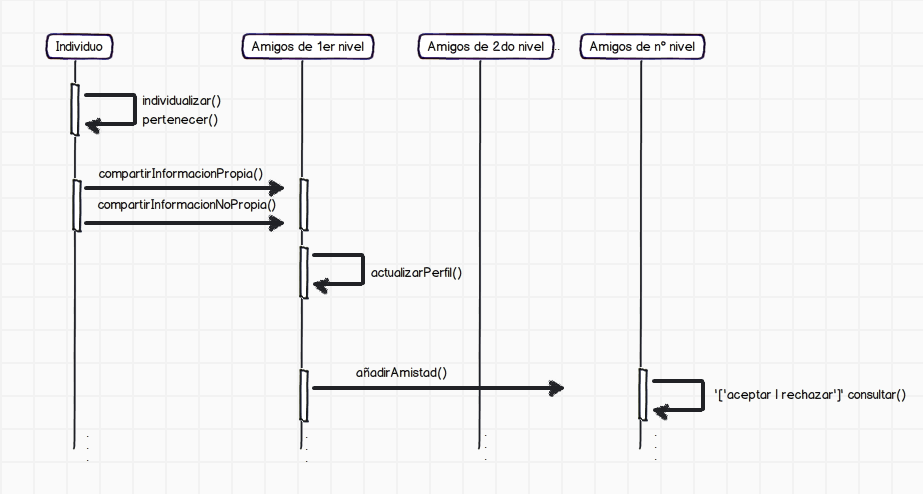
\includegraphics[angle=90,width=0.7\textwidth]{figure/fig_socialFlowDiagram.PNG}
			\newline
			\textbf{Fuente:} Elaboraci\'on propia de representaci\'on de \ac{FOAF} en un
			Diagrama de Flujos (Diagrama \ac{UML}).
		\label{fig:SocialFlowDiagram}	
	\end{figure}
	
	\section{An\'alisis y Dise\~no: Modelado}
	\label{sec:modelling}
	En esta secci\'on se abarcar\'a todas las bases par realizar el an\'alisis y
	dise\~no de una aplicaci\'on social basada en web, como se muestra en la Figura
	\ref{fig:SocialWebMLModelling} en el ciclo de vida de Social WebML se
	abarcar\'a las etapas de Dise\~no y/o Modelado de Base de Datos, Hipertexto y
	la Arquitectura.
	
	\begin{figure}[here]
		\centering
		\caption{Modelado: Social WebML Modelling}
		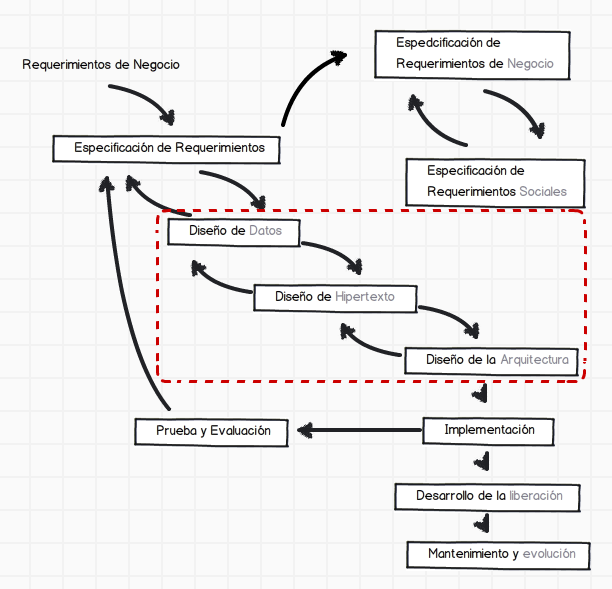
\includegraphics[width=1.0\textwidth]{figure/fig_SocialWebMLModelado.PNG}
			\newline
			\textbf{Fuente:} Elaboraci\'on propia basada en \textit{The extended WebML
			process}, visto por Frattini y Silva en \cite{Frattini2007}, p\'agina 81,
			Figura 24.
		\label{fig:SocialWebMLModelling}
	\end{figure}
	
		
		\subsection{Modelado de la Base de Datos}
		\label{sec:proposalDB}
		
		\begin{figure}[here]
			\centering
			\caption{Propuesta: Base de Datos (Inicial) para Social WebML}
			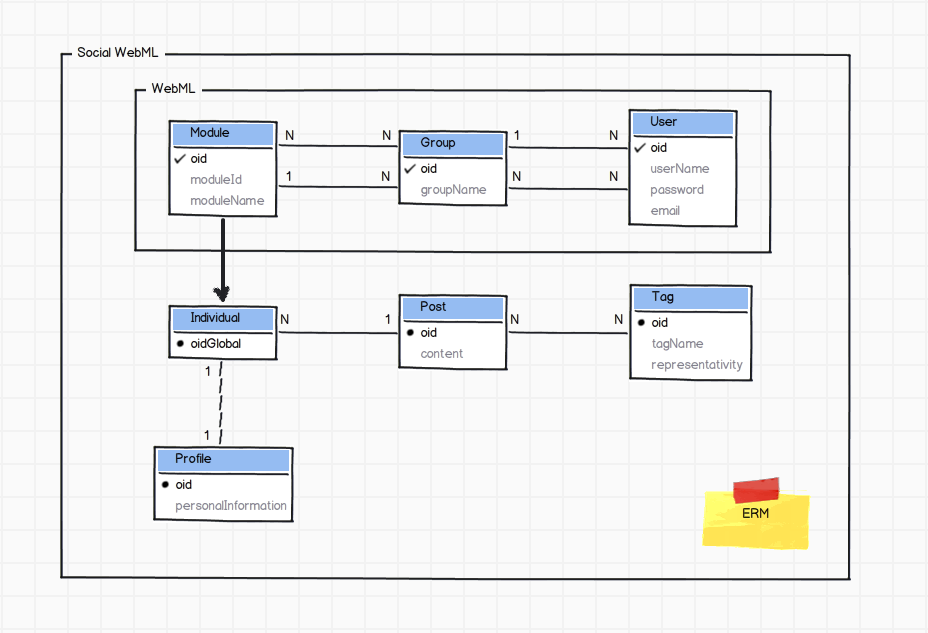
\includegraphics[angle=90,width=1.0\textwidth]{figure/fig_proposalBD.png}
			\newline
			\textbf{Fuente:} Elaboraci\'on propia de la extensi\'on de la Base de
			Datos inicial para Social WenML basado en la Base de Datos inicial de
			\ac{WebML}.
			\label{fig:proposalDB}
		\end{figure}
			  
		Como se puede ver en la Figura \ref{fig:proposalDB} se esta dividiendo en $2$
		conjuntos ``l\'ogicos'', los cuales representan la visi\'on actual de
		\ac{WebML} y la propuesta de este trabajo, siendo etiquetadas las mismas en el
		gr\'afico.
		
		En el conjunto \textbf{Social WebML} se propone un total de $4$ tablas,
		etiquetadas con los nombres:
		
		\begin{itemize}
		  \item Tag
		  \item Post
		  \item Individual 
		  \item \textbf{Profile}
		\end{itemize}
		
		Para poder explicar este \ac{ERM} se tiene que tener presente que se esta
		utilizando una notaci\'on \ac{UML} comentada por Bongio et al. en
		\cite{Ceri2003}, la cual se lee de forma inversa a la forma tradicional de
		lectura \ac{ERM}\footnote{Por ejemplo: la relaci\'on \ac{UML} entre la tabla
		Individual y Post es $N \to 1$, la cual significa: que \textbf{1} elemento de
		la tabla Individual posee relaci\'on con \textbf{N} elementos de la tabla Post
		y \textbf{1} elemento de la tabla Post posee relaci\'on con \textbf{1} elemento
		de la tabla Individual.}.
		
		Se pasar\'a a explicar el porque de cada una de estas tablas, comenzando desde
		la tabla \textbf{Individual}, como se puede ver se esta usando herencia de
		tablas, el cual como lo indica Maier y Zdonik en \cite{Zdonik1990} cuando se
		refiere a la herencia de tipos en bases de datos orientadas a objetos, en este
		caso se agregar\'a todos los elementos de la tabla padre a la tabla hija
		(tabla heredada) adicion\'andole ciertas caracter\'isticas (ciertos
		atributos), al igual como si de ``Herencia de Clases'' se tratase, el cual
		Fowler en \cite{Fowler2003} explica al referirse a \textbf{sub--classing}, el
		atributo el cual se esta adicionando es \textit{\textbf{oidGlobal}}, el cual
		almacenar\'a un identificador \'unico, no solo a nivel de aplicaci\'on sino a
		nivel web, este actualmente se le considera el identificador generado por el
		est\'andar OpenSocial, como se indica en \cite{OpenSocial} la finalidad de
		poseer un \'unico identificador es lograr un \'unico medio de acceso a la
		Internet o como Panzer y Smarr en \cite{Smarr2010} comentan, evitar dispersar
		la identidad y ser diferentes individuos para diferentes aplicaciones, en
		otras palabras la unificaci\'on de la identidad, lograr reconocer a un
		usuario: como un \textbf{individuo \'unico}, con sus problemas, con anhelos,
		sus deseos, etc. y de esta forma brindarle lo que quiere infiriendo esto desde
		su comportamiento.
		
		La Tabla \textbf{Profile} como se puede notar apenas consta de $2$ atributos y
		su relaci\'on con la tabla \textbf{Individual} es diferente a lo com\'unmente
		visto, esta tabla a diferencia de las tablas que ser\'an almacenadas en una
		base de datos, esta se considerar\'ia desde este punto como una tabla temporal
		o como Brambilla et al. \cite{Brambilla2003} le llaman: ``Virtual o Volatile
		Entity'', la cual almacenar\'a todos los objetos y/o entidades en el \'ambito de la
		sesi\'on de una aplicaci\'on o tambi\'en llamada memoria principal, en lugar de usar la
		base de datos para almacenar los atributos presentes en el modelo los cuales
		ser\'an obtenidos gracias a la informaci\'on que el \textbf{Individuo} (como
		se llamar\'a al usuario social desde ahora) permita compartir con el
		aplicativo y utilizados dependiendo de las necesidades y objetivos del
		aplicativo social.
		El atributo \textbf{\textit{oid}} indica en una relaci\'on $1 \to 1$ a que
		individuo en la red pertenece la informaci\'on que se esta capturando y el
		atributo \textbf{personalInformation} no representa solamente un atributo
		sino un conjunto de los mismos, los cuales ser\'an, como se dijo
		anteriormente, almacenados temporalmente dependiendo de las necesidades y objetivos del
		aplicativo social, con lo cual se brindar\'ia un servicio personalizado a cada
		individuo.
		
		La tabla \textbf{Post} como se puede notar esta relacionado con la tabla
		\textbf{Individual} en un relaci\'on $N \to 1$ es decir muchos \textit{post's}
		pueden ser hechos por un \underline{\'unico} \textit{individuo}, con esto
		se quiere dar a entender que un individuo puede expresar uno o muchos
		``contenidos'', siendo estos: ideas, im\'agenes, audios, videos, etc.
		dependiendo del contexto sobre el cual este desarroll\'andose  su interacci\'on,
		se dice interacci\'on, ya que mediante la \textbf{comunicaci\'on} de los
		contenidos antes nombrados es como los individuos sociales interact\'uan unos
		con otros, siendo esta la finalidad de la presencia de esta tabla en la cual
		cada contenido ``compartido'' pertenece \'unicamente a un individuo, pero
		sobre este puede existir una interacci\'on sobre otro individuo, el cual quiera
		compartir un contenido sobre el contenido antes nombrado, pero siempre
		guardando la unicidad entre un \textit{post} y el \textit{individuo} que lo
		comunic\'o. 
		
		%Anhadir comentario relacionado a los patrones sociales.
		%averiguar nombre de los tags @ de las redes sociales
		Por \'ultimo la tabla \textbf{Tag} relacionada indirectamente a la tabla
		\textbf{Post} ya que guardan una relaci\'on $N \to N$ guarda el mismo
		significado que actualmente se ve en los blogs, el cual se le adiciona el
		potencial de los ``hashtags o tags @\footnote{Los hashtags y los tags @ son
		m\'as utilizados desde la aparici\'on de Twitter, en la cual se utilizan los
		primeros para crear alg\'un tema de conversaci\'on o de seguimiento y los
		segundos para crear una referencia a alg\'un usuario en especial.}''
		de las redes sociales, con la cual se busca adem\'as de una referenciaci\'on,
		el cual complementa el objetivo de la tabla \textbf{Individual} y de esta
		forma obtener una representatividad, una marcada presencia del individuo dentro de
		la Web Social, no solo por quien es, sino tambi\'en por lo que hace.
		
		Gracias a estas $4$ tablas se logra a\~nadir el valor social al modelo de
		datos en \ac{WebML}, representado por:
		
		\fbox{\parbox[b]{\linewidth}{ 
		\begin{itemize}
		  \item Individualidad: Abstra\'ido gracias a la presencia de la tabla
		  \textbf{Individual} y \textbf{Profile}.
		  \item Comunicaci\'on: Conseguida a trav\'es de la presencia de la
		  interacci\'on de las tablas \textbf{Individual} y \textbf{Post}.
		  \item Referenciaci\'on y representatividad: Esto por una interacci\'on de
		  las tablas \textbf{Individual}, \textbf{Post} y en especial del enlace que
		  se logra por la presencia de la tabla \textbf{Tag}.
		\end{itemize}
		}}
		
		\subsection{Modelado del Hipertexto}
		\label{sec:proposalHypertext}
		
		\begin{figure}[here]
			\centering
			\caption{Propuesta: jerarqu\'ia de usuarios en Social WebML}
			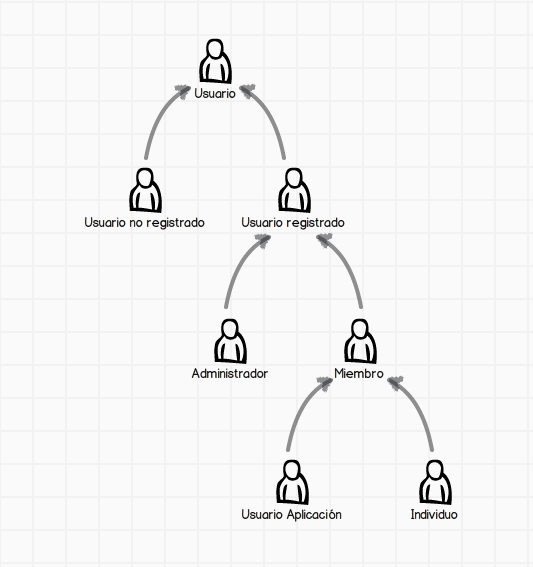
\includegraphics[width=0.9\textwidth]{figure/fig_proposalUserHierarchical.png}
			\newline
			\textbf{Fuente:} Elaboraci\'on propia basada en \textit{Example of group
			hierarchy diagram} vista por Bongio et al. en \cite{Ceri2003}, p\'agina
			211, Figura 7.2.
			\label{fig:proposalUser}
		\end{figure}
		
		En la Figura \ref{fig:proposalUser} se representa mediante un Diagrama de
		Casos de Uso el cual fue extendido por Bongio et al. en \cite{Ceri2003} para
		crear una jerarqu\'ia de actores y poder de esta forma dise\~nar hipertextos espec\'ificos para cada
		uno, inicialmente Frattini y Silva en \cite{Frattini2007} comentan que
		existir\'ia una jerarqu\'ia de actores de $3$ niveles siendo los hipertextos asociados los de:
		\textit{visitante o an\'onimo, miembro y administrador}; en el se
		extiende esta estructura para dise\~nar un nivel adicional
		disgregando al \textit{miembro} en $2$ actores adicionales que al ser
		heredados de este \'ultimo poseen todos sus atributos y adicionalmente se le a\~naden nuevos, estos son:
		\textbf{Usuario Aplicaci\'on} e \textbf{Individuo}; el primero para soportar
		todas las interacciones tradicionales de las aplicaciones web en donde la
		comunicaci\'on entre la p\'agina web y el usuario era o uni o bi--direccional,
		conservando as\'i la posibilidad de mantenerse an\'onimo seg\'un sea la
		necesidad del usuario, y la presencia del actor \textit{Individuo} ya nos
		brinda la idea de la existencia de un ambiente de desenvolvimiento o, la de un
		hipertexto de tipo social. Se mantuvo la existencia del actor \textit{Usuario
		Aplicaci\'on} conjunta con \textit{Individuo} para, en una primera instancia
		proveer del poder de decisi\'on al individuo de: que y como querer comportarse
		durante su viaje por el mundo de la Social Web, pero como lo dijo
		O'Reilly en \cite{OReilly2007} se debe de llegar a un punto en el cual exista
		la computaci\'on ubicua, en donde no se pueda notar la diferencia de la
		conexi\'on con el mundo virtual, hacerlo mas llevadero y por lo tanto hacer
		m\'as placentero este viaje, para ello es que la entrada del aspecto social el
		cual ayude a brindar una personalizaci\'on de servicios es muy importante.
		
		\begin{figure}[here]
			\centering 
			\caption{Propuesta: Unidades Sociales}
			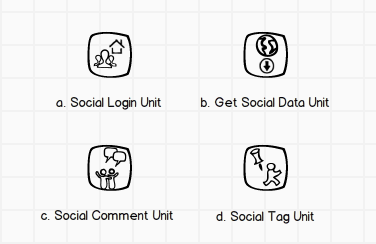
\includegraphics[width=0.8\textwidth]{figure/fig_SocialUnits.png}
			\newline
			\textbf{Fuente:} Elaboraci\'on propia para la representaci\'on de
			unidades sociales asociadas al comportamiento de los grupos definidos
			para el Modelado del Hipertexto.
			\label{fig:proposalSocialUnits}
		\end{figure}
	
		En la Figura \ref{fig:proposalSocialUnits} se puede identificar los aspectos
		sociales que se implementar\'an para esta propuesta, mediante el dise\~no y
		codificaci\'on de las Custom Units (cuyo nombre son los que recibe la
		creaci\'on de nuevas unidades de contenido y/o de operaci\'on en el \ac{CASE}
		WebRatio siendo estas Ad--hoc a las necesidades del programador), los cuales son:
		
		\begin{itemize}
		  \item[a.] \textbf{Social} Login Unit
		  \item[b.] Get \textbf{Social} Data Unit
		  \item[c.] \textbf{Social} Comment Unit
		  \item[d.] \textbf{Social} Tag Unit
		\end{itemize}
				
		En el caso de \textbf{Social Login Unit} esta tiene como finalidad proveer al
		dise\~no de hipertexto de la caracter\'istica social de \textbf{Individualidad}
		la cual mediante la implementaci\'on de OpenSocial se utilizar\'a o en
		determinados casos se generar\'a el uso de un \'unico individuo desde y para
		la aplicaci\'on.
		
		La finalidad de la unidad \textbf{Get Social Data Unit} fue la previa
		utilizaci\'on de la unidad \textit{Social Login Unit} de la cual se
		extraer\'ia una conexi\'on hacia la informaci\'on gen\'erica del individuo almacenado en
		la sesi\'on y de la cual dependiendo del negocio del aplicativo extraer
		informaci\'on relevante para el usuario y para el aplicativo, la cual
		previamente el individuo acept\'o compartir con los dem\'as, que pudiese
		ayudar a personalizar el contenido brindado por la aplicaci\'on social.
		
		Para \textbf{Social Comment Unit} se tiene como base brindar una opci\'on de
		soluci\'on a la caracter\'istica social de \textit{Comunicaci\'on many-to-many}
		``desde, hacia y por'' el individuo que haga uso de una determinada aplicaci\'on
		social.
		
		Finalmente para el caso del \textbf{Social Tag Unit} la caracter\'istica de la
		\textit{Referenciaci\'on} fue la base para su dise\~no en la cual busca una
		representatividad tanto del individuo como de su forma de ser y actuar, lo cual
		le brinda con el tiempo una identidad m\'as representativa y \'unica.
		
		%\subsection{Modelado de la Arquitectura}
		%\label{sec:proposalArchytectural}
		%-------------------------
	\section{Construcci\'on}
	\label{sec:construction}
	En esta secci\'on se mostrar\'a el desarrollo e implementaci\'on de los
	componentes sociales (Custom Units) para la presente propuesta:
	
	\begin{itemize}
	  \item[a.] \textbf{Social} Login Unit
	  \item[b.] Get \textbf{Social} Data Unit
	  \item[c.] \textbf{Social} Comment Unit
	  \item[d.] \textbf{Social} G Maps Unit
	\end{itemize}
	
	Con respecto a la secci\'on anterior se puede notar que no se implmentar\'a la
	Custom Unit \textit{Social Tag Unit} ya que para efectos de reutilizaci\'on de
	componentes se utilizar\'a el Custom Unit implementada por De Andreis en
	\cite{Andreis2010}, como se puede ver en la Figura \ref{fig:NuvulaDiTags} se
	muestra el como debiera ser la implementaci\'on, en el modelado del hipertexto,
	de esta unidad.
		
		\begin{figure}[here]
			\centering 
			\caption{Custom Unit: Tag Unit}
			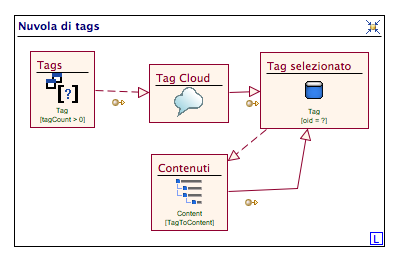
\includegraphics[width=0.6\textwidth]{figure/fig_NuvulaDiTags.png}
			\newline
			\textbf{Fuente:} Proyecto
			WRCommunity\footnote{http://code.google.com/p/webratio-community-patterns/}:
			Componente \textit{Tag Cloud Unit}.
			\label{fig:NuvulaDiTags}
		\end{figure}

	Para el desarrollo de estas \textit{Social} Custom Units nos hemos basado en 3
	fuentes, la $1^a$ es el wiki de
	WebRatio\footnote{http://wiki.webratio.com/index.php/Custom\_Unit\_Guide}, en
	la cual se brinda una breve descripci\'on, en palabras de los desarrolladores de
	WebRatio, de la forma adecuada de implementar Custom Units; como $1^a$ fuente
	nos basaremos en el \textit{Appendice A: Realizzare unit\`a personalizzate in
	WebRatio} del trabajo realizado por De Andreis en \cite{Andreis2010}, el cual
	se le sufrio un versionamiento adicionandole algunos aspectos importantes como
	por ejemplo que para el dise\~no de la capa visual no era necesario a\~nadir
	c\'odigo complicado para su correcto funcionamiento (este trabajo juega un
	papel importante en el trabajo, pero al no ser objeto de estudio de la
	propuesta se a\~nade en el Anexo \ref{ane:customUnits}) y como fuente final el
	GoogleGroup de
	WebRatio\footnote{https://groups.google.com/forum/?fromgroups\#!topic/webratio/rGeLxDCJELY}
	ahora migrado a WebRatio Forum\footnote{http://forum.webratio.com/}.
	
	Con respecto a la configuraci\'on inicial de estas unidades se tiene que
	enfatizar que estas Custom Units no ser\'an solamente unidades de contenido
	(en otras palabras no solo mostraran alguna referencia visual en el aplicativo)
	y tampoco ser\'an solamente unidades de operaci\'on, las cuales se encarguen en
	background de realizar alguna acci\'on sobre el aplicativo, sino que ser\'an de
	ambos tipos, es por ello que como podemos ver en la Figura
	\ref{fig:configCustomUnit} en la secci\'on \textit{Type}, continuando en las configuraciones generales de
	las Custom Units tambi\'en se tiene que tener en cuenta la propiedad
	\textit{Default Link to Operation} el cual debe de poseer como atributo el
	valor \textit{transport} para que de esta forma la informaci\'on viaje por la
	sesi\'on y no se pierda en la unidad misma, las otras propiedades son
	importantes para el dise\~no de Custom Units de contenido por ello tambi\'en
	las resaltamos, ya que como se coment\'o las \textit{Social} Custom Units de la
	presente propuesta cumplira ambos roles; el der una unidad de contenido y el de
	ser una unidad de operaci\'on.
	
	\begin{figure}[here]
		\centering 
		\caption{Custom Unit: Configuraci\'on de Propiedades Generales}
		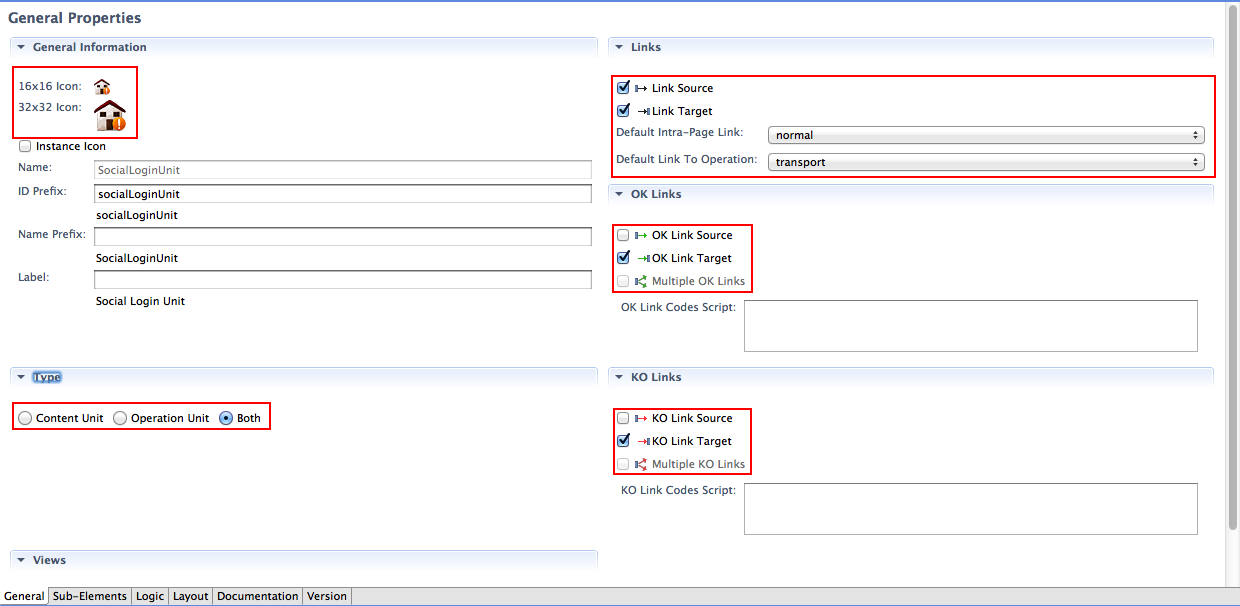
\includegraphics[angle=90,width=0.7\textwidth]{figure/dev/fig_SocialLoginUnit_dev.png}
		\newline
		\textbf{Fuente:} Elaboraci\'on Propia basada en las configuraciones
		mostradas por De Andreis en \cite{Andreis2010}.
		\label{fig:configCustomUnit}
	\end{figure}
	
	Con lo anteriormente expuesto la configuraci\'on general del modelado de las
	Social Custom Units est\'a finalizado, para acabar con la configuraci\'on
	inicial de la unidad, previa a la codificaci\'on del comportamiento que debe
	poseer la unidad, se debe modificar (si fuera necesario) los \textit{input y
	output templates}, un ejemplo de ellos se muestra a continuac\'on:
	
\begin{lstlisting}[language=xml, style=eclipse]
	#?delimiters <%,%>,<%=,%>
	<%
	setXMLOutput()
	def unitId = unit.valueOf("@id")
	%>
	
	<OutputParameters>
	  <OutputParameter name="myResult" type="" label="myResult"/>
	  <OutputParameter name="uid" type="" label="uid"/>
	  <OutputParameter name="name" type="" label="name"/>
	</OutputParameters>      
\end{lstlisting}

	A continuaci\'on se debe de codificar 2 aspectos:
	\begin{itemize}
	  \item \textbf{El comportamiento de background} de la Custom Unit, el cual es
	  codificado en
	  \textit{Java}\footnote{http://www.oracle.com/technetwork/java/index.html} o
	  en \textit{Groovy}\footnote{http://groovy.codehaus.org/}.
	  \item \textbf{El comportamiento visual}, el cual puede ser codificado
	  enteramente en \textit{html}, \textit{css}, \textit{javascript}, \textit{jsp}, entre otros,
	  adicionalmente utilizando un conjunto de tags \textit{jstl} propios de
	  Webratio, con lo cual se maneja una inter--conexi\'on entre las diferentes
	  capas de la arquitectura de WebRatio.
	\end{itemize}
	
	En el Anexo \ref{ane:srcCustomUnits} se muestra la codificaci\'on realizada
	para cada Social Custom Unit.
	
	Para poder realizar el dise\~no y modelado de las Social Custom Units se
	tomaron ciertos aspectos importantes, estas son descritas y mejor explicadas en
	la Tabla \ref{tab:customUnits} donde se ve el nombre que se le brindo a la
	unidad, los patrones sociales de dise\~no en que fue basado, el tipo de unidad
	que representa, si es unidad de contenido o unidad de operaci\'on y una breve
	descripci\'on de la misma en el campo funcionalidad.

	\begin{table}[htbp]
	\centering
	\caption{Unidades Sociales}
		\begin{tabular}{|l|p{12cm}|}
			\hline
			\multicolumn{2}{|c|}{--\textbf{Social Login Unit}--}					\\\hline 
			\textbf{Patrones Sociales}	&	Aggregation -- Mashup					\\
										&	Permission setting 						\\
										&	Permission check 						\\\hline
			\textbf{Tipo}				&	Content Unit \& Operation Unit			\\\hline
			\textbf{Imagen} & 
\includegraphics{units/SocialLoginUnit.png}			\\\hline
			\textbf{Funcionalidad}		&	Acceso a la aplicaci\'on brindando acceso a
			ciertos datos personales del individuo social, que permitan a la
			aplicaci\'on brindar un servicio personalizado al individuo.			\\\hline
			
			\multicolumn{2}{|c|}{--\textbf{Get Social Data Unit}--}					\\\hline 
			\textbf{Patrones Sociales}	&	Aggregation -- Mashup					\\
										&	Social visualization					\\
										&	Permission setting						\\
										&	Permission check						\\
										&	Importation								\\\hline
			\textbf{Tipo}				&	Content Unit \& Operation Unit			\\\hline 
			\textbf{Imagen} & 
\includegraphics{units/GetSocialDataUnit.png}			\\\hline
			\textbf{Funcionalidad}		&	Extrae cierta informaci\'on del individuo social
			que accedi\'o a la aplicaci\'on con las credenciales de una red
			social.																	\\\hline
			
			\multicolumn{2}{|c|}{--\textbf{Social Comment Unit}--}					\\\hline 
			\textbf{Patrones Sociales}	&	Aggregation -- Mashup					\\
										&	Social visualization					\\
										&	Permission setting						\\
										&	Permission check						\\
										&	Publication								\\
										&	Talk									\\
										&	Notification							\\\hline 
			\textbf{Tipo}				&	Content Unit \& Operation Unit			\\\hline
			\textbf{Imagen} & 
\includegraphics{units/SocialCommentUnit.png}			\\\hline 
			\textbf{Funcionalidad}		&	Permite usar alguna informaci\'on del individuo
			social que accedi\'o al aplicativo para que el pueda expresar sus
			impresiones sobre un determinado hecho.									\\\hline
			
			\multicolumn{2}{|c|}{--\textbf{Social G Maps Unit}--}					\\\hline 
			\textbf{Patrones Sociales}	&	Aggregation -- Mashup					\\
										&	Social visualization					\\
										&	Permission setting						\\
										&	Permission check						\\\hline 
			\textbf{Tipo}				&	Content Unit \& Operation Unit			\\\hline 
			\textbf{Imagen} & 
\includegraphics{units/SocialGMapsUnit.png}			\\\hline
			\textbf{Funcionalidad}		&	Usando cierta informaci\'on del individuo social
			que accedi\'o a la aplicaci\'on permite mostrar las relaciones de amistad
			existente a nivel mundial del individuo social.							\\\hline
		\end{tabular}
	\newline
	Fuente: Elaboraci\'on propia -- Unidades Sociales dise\~nadas para el
	Dise\~no de Hipertexto.
	\label{tab:customUnits}
	\end{table}
			
 				
\chapter{CASO DE ESTUDIO}	
\label{chap:studyCase}	
En este cap\'itulo se presenta un caso de estudio did\'actico para describir el
uso de la metodolog\'ia Social WebML en el desarrollo de la aplicaci\'on
\textit{``WebRatio Travel Agency''}, esta aplicaci\'on estar\'a basada
inicialmente en el portal de una agencia de viajes, la cual estar\'a
complementada con el paradigma social implementado desde la propuesta de Social
WebML.

	\section{Contexto}
	\label{sec:context}
	\textbf{Web Ratio Travel Agency (WRTA)} es una agencia de viajes que brinda
	el servicio de informaci\'on y reservaci\'on a sus clientes desde su p\'agina web. 
	En esta p\'agina un usuario puede ver todos los aspectos acerca de los viajes
	ofertados por la agencia, por ejemplo: \textit{viajes, reservaciones, costos,
	fechas, etc.}; adicional puede recibir noticias, promociones por temporada,
	etc.
	Actualmente WRTA se siente en la necesidad de brindar un servicio m\'as
	personalizado a sus clientes, como por ejemplo permitir a sus clientes
	\textbf{comentar} y \textbf{recomendar} los lugares hacia donde han ido y
	sobre todo el servicio que han utilizado y de esta manera lograr promocionar el
	servicio que brindan. 
	Principalmente por estas razones es que WRTA ha decidido adicionar ciertas
	funcionalidades que le permitan cubrir las necesidades que sus clientes
	desean para lo cual se har\'a uso de la metodolog\'ia de desarrollo \ac{WebML}
	y Social WebML con lo cual cubriremos las necesidades de negocio y las
	necesidades sociales, identificadas en primera instancia, por WRTA.
	
	\section{WRTA - An\'alisis de Requerimientos del Negocio}
	\label{sec:reqAnalysis}
		
	En esta secci\'on se realizar\'a la identificaci\'on de actores, grupos  y
	escenarios de desarrollo de sus funciones.
	
	Inicialmente para la aplicaci\'on se presenta la existencia de los actores
	\textbf{administrador} y \textbf{usuario} en si mismos.
	
	\begin{itemize}
	  \item \textbf{Administrador: } Actor a cargo de la administraci\'on de
	  la aplicaci\'on en su totalidad.
	  \item \textbf{Usuario: } Actor el cual puede revisar informaci\'on referente
	  a viajes, realizar operaciones sobre los mismos como reservas, petici\'on de
	  informaci\'on, etc.
	\end{itemize}
	
		\subsection{Identificaci\'on de grupos}
		\label{ssec:groupIdentification}
		Para la identificaci\'on de los grupos se tomar\'a como base los actores
		previamente identificados adicion\'andole la presencia de un actor de tipo
		\textbf{an\'onimo}, los cuales tomar\'an el nombre de grupos.

		\begin{itemize}
		   \item \textbf{Grupo -- Administrador: } Registro pre--existente en la
		   aplicaci\'on con el rol de \textit{Admin}.
		   \item \textbf{Grupo -- Usuario: } Registrado por si mismo en la
		   aplicaci\'on.
		   \item \textbf{Grupo -- (Usuario) An\'onimo: } No registrado en la
		   aplicaci\'on y limitado a la visibilidad de ciertos contenidos.
		\end{itemize}
		  
		\begin{table}[htbp]
		\centering
		\caption{WRTA: Descripci\'on de Grupos}
			\begin{tabular}{|l|l|}
				\hline
				\multicolumn{2}{|c|}{\textbf{GRUPOS}} \\\hline
				\multicolumn{2}{|c|}{\textbf{Grupo -- Administrador}} \\\hline
				Descripci\'on		& Administraci\'on de la aplicaci\'on en su totalidad.\\\hline 
				Escenarios			& Acceso al SiteView de Administrador.					\\
									& Inscripci\'on \underline{de} viajes.					\\
									& Inscripci\'on \underline{de} promociones.				\\
									& Inscripci\'on \underline{de} descuentos.				\\
									& Administraci\'on del ciclo de vida de un viaje.		\\\hline
			    Data Profile 		& UserName, Password, Email.							\\\hline 
				Acceso de lectura   & Informaci\'on de viajes y de usuarios.				\\\hline
				Acceso de escritura & Informaci\'on de viajes y de usuarios.				\\\hline
				\multicolumn{2}{|c|}{\textbf{Grupo -- Usuario}} \\\hline
				Descripci\'on 		& Agrupa los usuarios que se registran en la
				aplicaci\'on.\\\hline 
				Escenarios 			& Acceso al SiteView de Usuario.							\\
									& Inscripci\'on \underline{a} un viaje: normal,
									promoci\'on o descuento.								\\\hline 
				Data Profile 		& UserName, Password, Nombre, Apellido, Email.			\\\hline
				Acceso de lectura	& Informaci\'on de viajes.								\\\hline
				Acceso de escritura & Informaci\'on de usuario (limitado a su propia
				informaci\'on). 																\\\hline
				\multicolumn{2}{|c|}{\textbf{Grupo -- (Usuario) An\'onimo}} \\\hline
				Descripci\'on 		& Agrupa a los visitantes o personas no registradas.    \\\hline
				Escenarios 			& Acceso al SiteView de Visitante.						\\
									& Registro de usuario.									\\\hline
				Data Profile 		& Perfil no requerido.									\\\hline 
				Acceso de lectura	& Informaci\'on de la empresa.							\\\hline
				Acceso de escritura & Ninguna												\\\hline
				
			\end{tabular}
			\newline
			\textbf{Fuente:} Elaboraci\'on Propia para describir aspectos
			importantes acerca de los Grupos/Usuarios elementales del aplicativo
			WRTA.
			\label{tab:descriptionTable}
		\end{table}
		
		
		En la Tabla \ref{tab:descriptionTable} se presenta cada grupo con un poco
		m\'as de detalle, siendo el campo \textit{Descripci\'on}: la principal
		acci\'on a realizar por los integrantes del grupo, \textit{Escenarios}
	    representa las acciones generales a realizarse por defecto dentro del
	    grupo (los cuales representan a los requerimientos
	    funcionales\footnote{Algunos de estos requerimientos podr\'ian ser
	    desconocidos u obviados durante una primera sesi\'on de an\'alisis, sin
	    embargo como se explico en la Figura \ref{fig:WebML_LifeCicle},
	    \ac{WebML} es un proceso iterativo, por consiguiente en sesiones
	    posteriores se identificar\'ian requerimientos adicionales si estas fuesen
	    necesarias.} en el aplicativo), \textit{Data Profile}: la informaci\'on
	    resaltante a ser almacenada acerca de cada uno de lo integrantes de este grupo,
	    \textit{Accesos de lectura y escritura} se refiere a la facultad que posee
	    el grupo de poder acceder a la informaci\'on almacenada en la aplicaci\'on
	    ya sea solo para visualizaci\'on o modificaci\'on.
	    
		\subsection{An\'alisis de Requerimientos Funcionales}
		\label{ssec:functionalReq}
		
		\begin{figure}[here]
			\centering 
			\caption{WRTA: jerarqu\'ia de Grupos}
			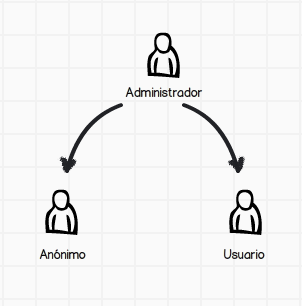
\includegraphics[width=0.5\textwidth]{figure/fig_WRTA_Hierarchy.png}
			\newline
			\textbf{Fuente:} Elaboraci\'on propia basada en \textit{Example of group
			hierarchy diagram} vista por Bongio et al. en \cite{Ceri2003}, p\'agina
			211, Figura 7.2.
			\label{fig:WRTA_Hierarchy} 
		\end{figure}
	    
	    En la Figura \ref{fig:WRTA_Hierarchy} se presenta en un Diagrama de Casos
	    de Uso que representa la jerarqu\'ia de los actores que intervienen en la
	    aplicaci\'on, siendo agregado el usuario an\'onimo, de los cuales los nodos
	    en esta jerarqu\'ia representan lo que se convertir\'a en los
	    \textit{SiteView} en el modelado del hipertexto.
	    
	    En la Tabla \ref{tab:descriptionTable} se present\'o el campo
	    \textbf{Escenarios} mediante la cual se realizar\'ia la primera captura de
	    requerimientos funcionales, para lo cual se har\'a uso de los grupos y los
	    escenarios en los cuales estos interact\'uan, esto se har\'a mediante la
	    utilizaci\'on de un Diagrama de Actividades visto por Ceri et al. en
	    \cite{Matera2003} en t\'erminos de \ac{UML}, en donde se podr\'a analizar
	    cada grupo por separado y su interacci\'on con los dem\'as.
	    
	    \begin{figure}[here]
			\centering 
			\caption{WRTA: Diagrama de Flujo entre grupos de actores}
			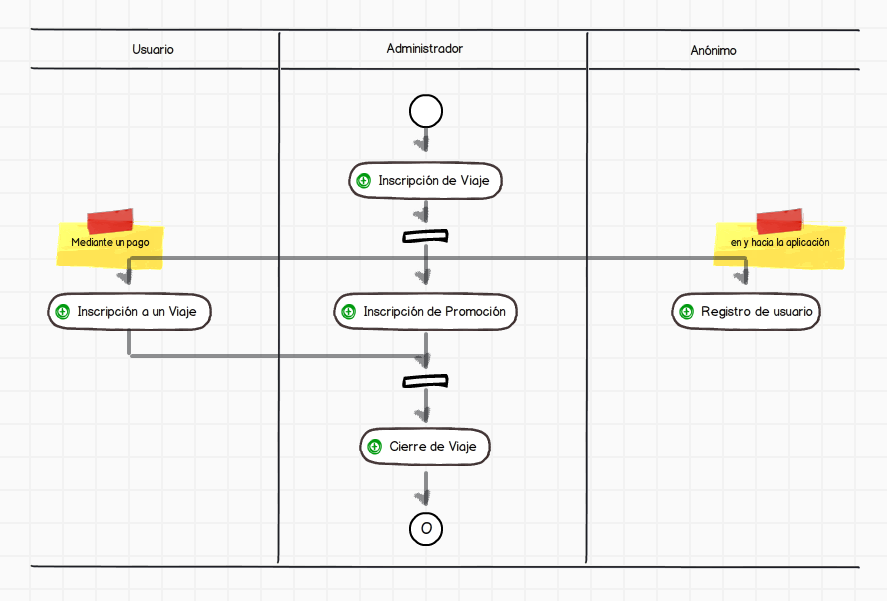
\includegraphics[width=0.9\textwidth]{figure/fig_WRTA_flowDiagram.png}
			\newline
			Fuente: Elaboraci\'on propia basada en el contexto del caso de estudio.
			\label{fig:WRTA_flowDiagram}
		\end{figure}

		En la Figura \ref{fig:WRTA_flowDiagram} se presenta la interacci\'on que poseen
		los grupos de usuario unos entre otros, as\'i como sus acciones principales (a
		transformarse en requerimientos funcionales) representados anteriormente con
		el nombre de \textit{Escenarios}.
 
	    
		\subsection{Identificaci\'on de Objetos Core de Informaci\'on}
		\label{ssec:coreObjects}
		Mediante la identificaci\'on de grupos y el an\'alisis de requerimientos
		funcionales se pudo distinguir $3$ objetos core de informaci\'on que despu\'es
		pasar\'an a ser parte de la etapa de modelado, estos son:
		
		\begin{itemize}
		  \item \textbf{Usuarios y grupos:} Representa la informaci\'on
		  fundamental acerca de los usuarios de la aplicaci\'on, los roles
		  pueden ser derivados de los grupos a los que ellos pertenecen as\'i
		  como sus permisos de lectura/escritura sobre diferentes objetos.
		  \item \textbf{Informaci\'on del Viaje:} Propiedades como: fechas de inicio y
		  fin de promociones, viajes, lugares, etc.
		  \item \textbf{Boletos o tickets:} Informaci\'on principal para la
		  administraci\'on de los viajes, objeto importante en la fase de
		  ``Inscripci\'on a un Viaje''.
		\end{itemize}
		
		\subsection{Identificaci\'on de SiteViews}
		\label{ssec:siteViews}
		En la Tabla \ref{tab:associationUG_SV} se refleja en m\'as detalle cada uno de
		los SiteViews presentes cuando se identific\'o los grupos de usuarios
		asociados a los escenarios o requerimientos funcionales de cada uno de ellos.
		
		\begin{table}[htbp]
		\centering
		\caption{Relaci\'on entre los SiteViews (Grupos) con Requerimientos
		Funcionales}
			\begin{tabular}{|l|l|l|}
			\hline
			Administrador	& Usuario	& An\'onimo\\ \hline
			Acceso al SV\footnote{SV = SiteView} de Administraci\'on & Acceso al SV de
			Usuario & Acceso al SV de Visitante \\\hline
			Inscripci\'on de un Viaje &
			Inscripci\'on a un Viaje & Registrarse como usuario \\\hline
			Inscripci\'on de una Promoci\'on & Inscripci\'on a una Promoci\'on &
			\multicolumn{1}{c|}{---}\\
			\hline Administraci\'on del Viaje & \multicolumn{1}{c|}{---} & \multicolumn{1}{c|}{---}
			\\
			\hline
			\end{tabular}
		\newline
		Fuente: Elaboraci\'on propia basada en las acciones relacionadas entre los
		actores.
		\label{tab:associationUG_SV}
		\end{table}
		
	\section{WRTA - An\'alisis de Requerimientos Sociales}
	\label{sec:socReqAnalysis}
	En esta secci\'on se realizar\'a un complemento al an\'alisis de
	requerimientos de negocio para a\~nadirle el paradigma social.
	
		\subsection{Identificaci\'on de Grupos -- Sociales}
		\label{ssec:socialGroup}
		En la Figura \ref{fig:WRTA_Hierarchy} se present\'o el modelo jer\'arquico de
		grupos para WRTA, en esta secci\'on se realizar\'a una actualizaci\'on al
		Diagrama de Casos de Uso utilizado para representar un aspecto social dentro
		de WRTA, en la cual se utiliza los t\'erminos \textit{Visitante}, en lugar de
		\textit{An\'onimo} y el  actor (grupo) \textit{Usuario} se ha dividido en $2$
		grupos ``simb\'olicos'', se utiliza el t\'ermino simb\'olico ya que en
		realidad la divisi\'on de este grupo no significara la divisi\'on en $2$
		SiteViews como se hizo con los dem\'as grupos sino que la informaci\'on de
		cada grupo ser\'a tratada de forma diferente, como se puede ver en la Figura
		\ref{fig:WRTA_SocialHierarchy} estos actores (grupos) son:
		 
		\begin{figure}[here]
			\centering 
			\caption{WRTA: jerarqu\'ia de Grupos v2.0 -- Grupo Social}
			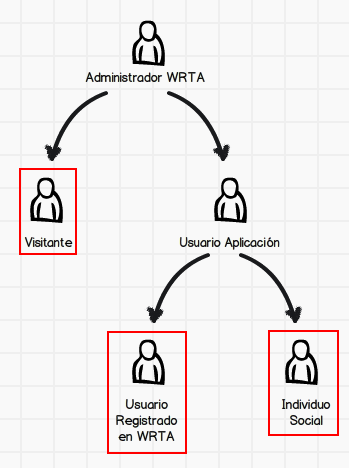
\includegraphics[width=0.45\textwidth]{figure/fig_WRTA_Socialhierarchy.png}
			\newline
			\textbf{Fuente:} Elaboraci\'on propia basada en \textit{Example of group
			hierarchy diagram} vista por Bongio et al. en \cite{Ceri2003}, p\'agina
			211, Figura 7.2.
			\label{fig:WRTA_SocialHierarchy}
		\end{figure} 
				
		\begin{itemize}
		  \item \textbf{Usuario Registrado en WRTA:} Este grupo es representado por
		  las personas que deseen guardar su identidad global para otros fines y se
		  inscriben de forma tradicional a la aplicaci\'on brindando solo cierta
		  informaci\'on al aplicativo y recibiendo un tratamiento del mismo de forma
		  tradicional.
		  \item \textbf{Individuo Social:} Este grupo esta representado por el
		  \textit{Individuo} Social que posee ya, una identidad en la Internet y desea
		  utilizar esta identidad para formar parte m\'as activa en la aplicaci\'on,
		  esto se logra a trav\'es de un acceso al aplicativo brindando credenciales
		  globales al aplicativo; por ejemplo O'Auth, Facebook Connect, etc.
		\end{itemize}

 
		Adicionalmente al realizar el an\'alisis de grupos se hizo un an\'alisis
		usando un Diagrama de Actividades, visto en la Figura \ref{fig:WRTA_flowDiagram},
		para representar los requerimientos funcionales representativos de la
		aplicaci\'on. Para complementar los requerimientos funcionales del aplicativo
		se a\~nade los requerimientos sociales, para WRTA se usar\'a los
		requerimientos sociales vistos anteriormente en la Figura
		\ref{fig:SocialFlowDiagram} en el Cap\'itulo \ref{chap:Proposal} de este trabajo.

	\section{WRTA - Dise\~no de Datos}
	\label{sec:dataDesign}
	Para el modelado de la base de datos se usar\'a como base el \ac{ERM} visto en
	la Figura \ref{fig:proposalDB}, esta estar\'a modelada con el \ac{IDE}
	WebRatio\footnote{http://www.webratio.com} como se puede ver en la Figura
	\ref{fig:WRTA_fig_WR_DataModel}.
 
	\begin{figure}[here]
		\centering 
		\caption{WRTA: Modelo (Inicial) de Base de Datos (Social) -- WebRatio}
		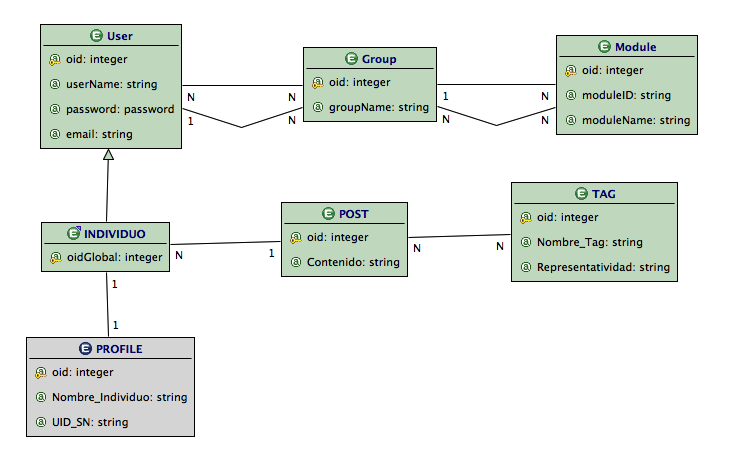
\includegraphics[width=0.8\textwidth]{figure/fig_WR_DataModel.png}
		\newline
		\textbf{Fuente:} Elaboraci\'on Propia -- Dise\~no del modelo de Base de Datos
		\label{fig:WRTA_fig_WR_DataModel}
	\end{figure} 
			
	En esta figura se muestra como se ha modelado la base de datos inicial
	mostrada anteriormente con WebRatio; se ha modelado las relaciones
	\textit{many--to--many}, ya que el \ac{IDE} transforma estas relaciones en
	sus respectivas relaciones \textit{one--to--many} y \textit{many--to--one} con
	la tabla intermedia respectiva de forma autom\'atica, como puede verse en la
	Figura \ref{fig:WRTA_fig_WR_autoModelling}, donde las Tablas: \textit{User},
	\textbf{Group}, \textbf{Module} y \textbf{TAG} se han transformado de forma
	autom\'atica en tablas \textbf{group\_module}, \textbf{tag\_post} y
	\textbf{user\_group}.
	
	\begin{figure}[here]
		\centering 
		\caption{WRTA: Mapeo Autom\'atico del \ac{ERM} -- WebRatio}
		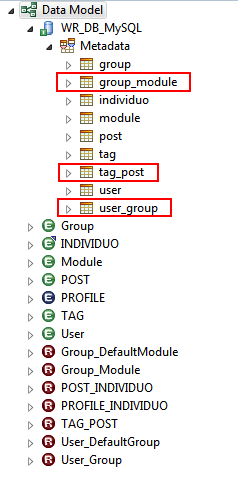
\includegraphics[width=0.4\textwidth]{figure/fig_WR_autoModelling.png}
		\newline
		\textbf{Fuente:} Elaboraci\'on Propia -- Dise\~no del modelo de Base de Datos
		(Relaciones)
		\label{fig:WRTA_fig_WR_autoModelling}
	\end{figure} 
	
	Algo importante a comentar es la existencia de la Tabla \textbf{PROFILE}, la
	cual posee una presentaci\'on distinta en el modelado, esto es porque se le ha
	cambiado un atributo en su estructura con la cual esta se vuelve una
	entidad vol\'atil\footnote{Como se coment\'o una entidad volatil es aquella
	la cual no se almacenar\'a en disco, sino que se almacenar\'a en memoria
	principal.}, espec\'ificamente para el \'ambito de la sesi\'on como se ve en la
	Figura \ref{fig:profileTableProperties}.
	
	\begin{figure}[here]
		\centering
		\caption{WRTA: Properties -- Tabla PROFILE}
		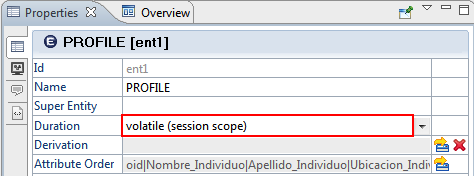
\includegraphics[width=0.5\textwidth]{figure/fig_profileProperties.png}
		\newline
		\textbf{Fuente:} Elaboraci\'on Propia -- Dise\~no del modelo de Base de Datos
		(Entidades)
		\label{fig:profileTableProperties}
	\end{figure}
	
	Para finalizar el modelado del Dise\~no de Datos, se a\~nade la parte
	funcional del aplicativo sobre la propuesta inicial de la Base de Datos de
	Social WebML. Como se puede ver en la Figura \ref{fig:WRTA_SocialDataModel} se han
	a\~nadido las tablas:
	
	\begin{itemize}
	  \item DESTINO
	  \item VIAJE
	  \item TICKET
	  \item TIPO\_VIAJE
	\end{itemize}
	
	Estas, basadas y a\~nadidas a la parte superior de \ac{WebML}, esto
	significar\'ia que la mayor\'ia de los requerimientos sociales a nivel de Base
	de Datos estar\'an en mayor proporci\'on ligadas a las tablas a\~nadidas para el
	desarrollo de la propuesta de Social WebML y los requerimientos funcionales a
	nivel de Base de Datos a las tablas cl\'asicas de \ac{WebML}.
	
	 \begin{figure}[here]
		\centering
		\caption{WRTA: Modelo (Final) de Base de Datos -- WebRatio}
		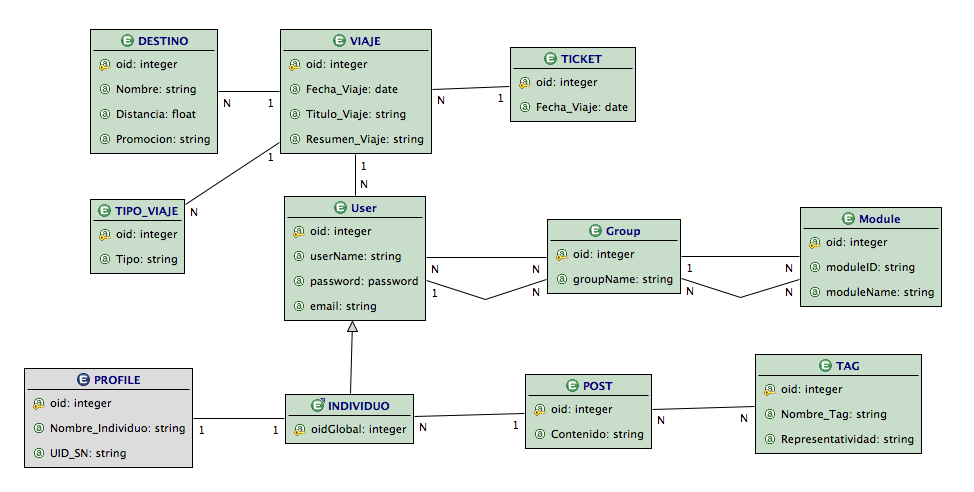
\includegraphics[width=1.0\textwidth]{figure/fig_WRTA_SocialDataModel.png}
		\newline
		\textbf{Fuente:} Elaboraci\'on Propia -- Dise\~no del modelo de Base de Datos
		\label{fig:WRTA_SocialDataModel}
	\end{figure}	
	
	En este modelo se agreg\'o la tabla \textbf{DESTINO} para almacenar los lugares
	hacia donde el cliente, usuario y/o individuo pudiera viajar utilizando el
	servicio brindado por WR Travel Agency. La tabla \textbf{TIPO\_VIAJE}
	representa una tabla de enumerativos donde se almacena todas las clases de viaje que WR Travel
	Agency maneje, como puede ser: \textit{simple, royal, empresarial, etc.} La
	tabla \textbf{VIAJE} representa una oferta de viaje hacia un determinado
	\textit{destino} con los \textit{tipos de viaje} ofertados para una fecha
	determinada con un costo dependiendo de las caracter\'isticas del viaje.
	Finalmente la tabla \textbf{TICKET} almacena la reservaci\'on de un cliente,
	usuario o individuo en una fecha determinada de un \textit{viaje}.
	
	 
	\section{WRTA - Dise\~no de Hipertexto}
	\label{sec:hypertextDesign}
	
	Esta secci\'on se basa en el an\'alisis socio/funcional visto
	en la Tabla \ref{tab:associationUG_SV} y Figura \ref{fig:WRTA_SocialHierarchy}
	en la cual se vio que se trabajar\'ia con un total de $3$ siteviews b\'asicos;
	como se puede ver en la Figura \ref{fig:WRTA_hypertextModel} en la parte
	inferior al \textbf{Data Model} se presentan $3$ siteviews representados en el
	\ac{IDE} WebRatio.
	
	Estos siteviews son:
	
	\begin{itemize}
	  \item P\'ublico
	  \item Administrador
	  \item Aplicaci\'on
	\end{itemize}
	
	\begin{figure}[here]
		\centering
		\caption{WRTA: Modelo de Hipertexto (SiteViews) -- WebRatio}
		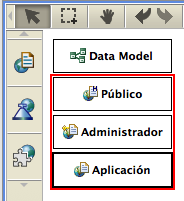
\includegraphics[width=0.3\textwidth]{figure/fig_WRTA_hypertextModel.png}
		\newline
		\textbf{Fuente:} Elaboraci\'on Propia -- Dise\~no del hipertexto de WRTA
		\label{fig:WRTA_hypertextModel}
	\end{figure}	
	
	
		\subsection{Siteview P\'ublico}
		\label{ssec:svPublico}
			
			El siteview de nombre \textit{P\'ublico} es el encargado de acoger a todo
			aquel cliente, usuario y/o individuo el cual no este registrado en la
			aplicaci\'on y/o a\'un no haya realizado un \textit{log--in}, por ello
			en el an\'alisis realizado se llamo grupo y/o usuario \textit{Visitante}.
			Como se puede ver en la Figura \ref{fig:WRTA_svPublico} el principal
			requerimiento funcional y social implementado es el de permitir el acceso a
			usuarios registrados en la aplicaci\'on y a Individuos Sociales (para este
			caso en particular, registrados en la Red Social Facebook).
			
			\begin{figure}[here]
				\centering
				\caption{WRTA: SiteView de acceso p\'ublico}
				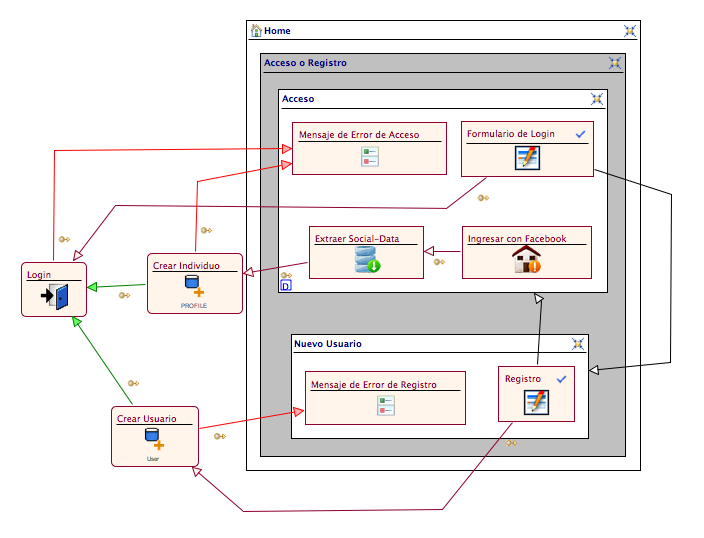
\includegraphics[width=1.0\textwidth]{figure/fig_WRTA_svPublico.png}
				\newline
				\textbf{Fuente:} Elaboraci\'on Propia -- Dise\~no del siteview p\'ublico
				\label{fig:WRTA_svPublico}
			\end{figure}	
			
			Para el desarrollo de este siteview se crearon $2$ p\'aginas: \textit{Acceso}
			y \textit{Nuevo Usuario} cuya funcionalidad es la de permitir o negar el
			acceso al aplicativo y la de registrar y acceder autom\'aticamente al
			aplicativo respectivamente.
			
			En la Tabla \ref{tab:svPublico} se presenta una relaci\'on entre las unidades
			de contenido, el tipo de unidad y la p\'agina a donde
			pertenecen, adem\'as de las unidades de operaci\'on las cuales no pertenecen
			a ninguna p\'agina.
					
			\begin{table}[htbp]
			\centering
			\caption{Unidades utilizadas para SiteView: P\'ublico}
				\begin{tabular}{|l|l|l|}
					\hline
					\textbf{P\'agina}	&	\textbf{Nombre Unidad}	&	\textbf{Tipo Unidad}\\\hline 
					Acceso			&	Formulario de Login			&	Entry Unit	\\\hline
					Acceso			&	Mensaje de Error de Acceso	&	Multi Message Unit\\\hline
					Acceso			&	Ingresar con Facebook		&	\textit{Social Login Unit}\\\hline
					Acceso			&	Extraer Social--Data		&	\textit{Get Social Data Unit}\\\hline
					Nuevo Usuario	&	Registro					&	Entry Unit	\\\hline
					Nuevo Usuario	&	Mensaje de Error de Registro&	Multi Message Unit\\\hline
					\multicolumn{1}{|c|}{---}&	Crear Usuario		&	Create Unit	\\\hline
					\multicolumn{1}{|c|}{---}&	Login				&	Login Unit	\\\hline
					\multicolumn{1}{|c|}{---}&	Crear Individuo		&	Create Unit	\\\hline
				\end{tabular}
			\newline
			Fuente: Elaboraci\'on propia -- Resumen de unidades de contenido y de
			operaci\'on para SiteView: P\'ublico.
			\label{tab:svPublico}
			\end{table}
			
			En la Figura \ref{fig:WRTA_paginaPublica} se puede ver como las unidades de
			contenido y operaci\'on interact\'uan y generan un modo de acceso de forma
			cl\'asica y una de tipo social, los cuales se enmarcaron en un cuadro rojo.
			
			\begin{figure}[here]
				\centering
				\caption{WRTA: Prototipo del siteView p\'ublico}
				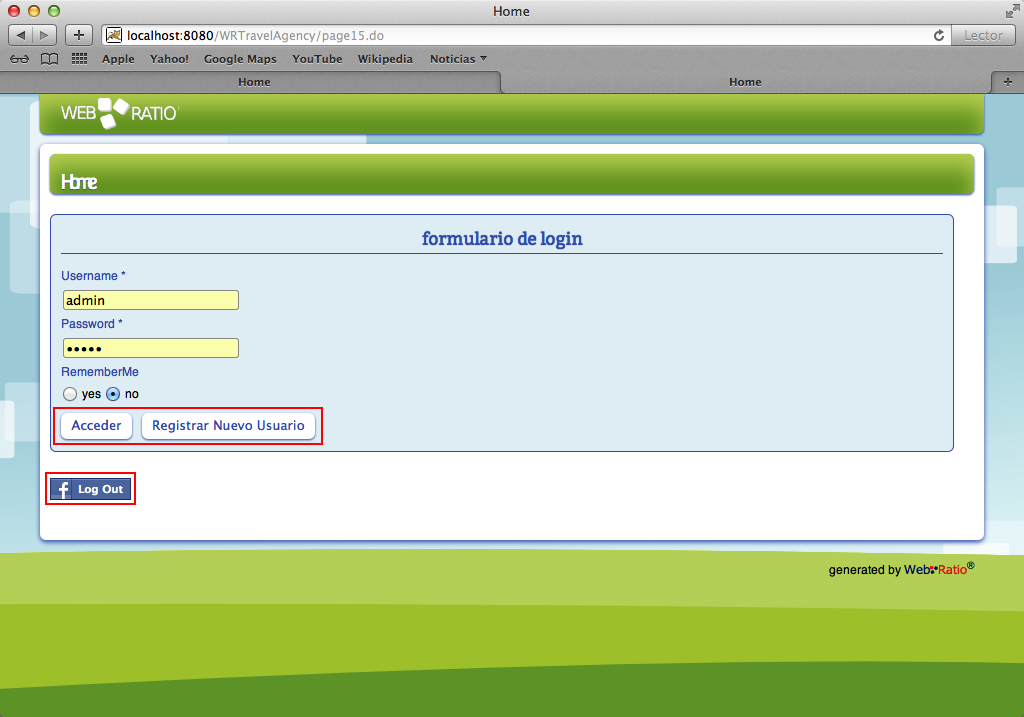
\includegraphics[width=1.0\textwidth]{figure/fig_WRTA_Publico.png}
				\newline
				\textbf{Fuente:} Elaboraci\'on Propia -- Prototipo en navegador del
				siteview p\'ublico
				\label{fig:WRTA_paginaPublica}
			\end{figure}
			
			
		\subsection{Siteview Administrador}
		\label{ssec:svAdministrador}
		
			El siteview de nombre \textit{Administrador} se encarga de proveer al
			aplicativo de las nuevas promociones, viajes, etc. Siendo los usuarios que
			tienen permitido el acceso, solo aquellos que pertenezcan al
			grupo de \textit{Administradores WRTA}.
			
			En la Figura \ref{fig:WRTA_svAdministrador} podemos ver representado el
			principal requerimiento funcional del siteview \textit{Administrador}, el cual
			es el registro de un Viaje.
	
			\begin{figure}[here]
				\centering
				\caption{WRTA: SiteView de acceso restringido para el administrador}
				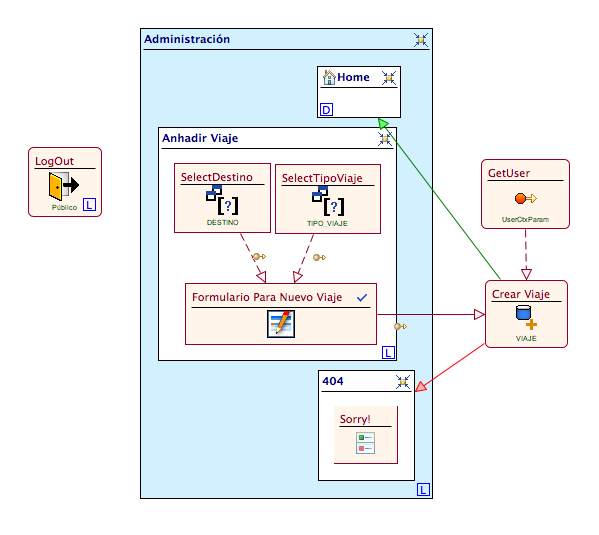
\includegraphics[width=1.0\textwidth]{figure/fig_WRTA_svAdministrador.png}
				\newline
				\textbf{Fuente:} Elaboraci\'on Propia -- Dise\~no del siteview Administrador
				\label{fig:WRTA_svAdministrador}
			\end{figure}
			
			
		 	En la Tabla \ref{tab:svAdministrador} se presenta una relaci\'on entre las unidades
			de contenido, el tipo de unidad y la p\'agina a donde
			pertenecen, adem\'as de las unidades de operaci\'on las cuales no pertenecen
			a ninguna p\'agina, en este siteview se hace menci\'on a $3$ p\'aginas de
			las cuales solo $2$ poseen un contenido, la raz\'on es que al momento de
			realizar un log--in exitoso el usuario Administrador ser\'a redirigido
			autom\'aticamente. la p\'agina  marcada con los atributos \textit{Home} y
			\textit{Default} ( marcado con: \fbox{D} en la parte inferior izquierda de
			las p\'aginas) y por consiguiente esta mostrar\'a en el landmark las dem\'as
			p\'aginas para su acceso.
		 	 
			\begin{table}[htbp]
			\centering
			\caption{Unidades utilizadas para SiteView: Administrador}
				\begin{tabular}{|l|l|l|}
					\hline
					\textbf{P\'agina}	&	\textbf{Nombre Unidad}	&	\textbf{Tipo Unidad}\\\hline 
					Anhadir Viaje		&	SelectDestino			&	Selector Unit\\\hline
					Anhadir Viaje		&	SelectTipoViaje			&	Selector Unit\\\hline 
					Anhadir Viaje		&	Formulario Para Nuevo Viaje&	Entry Unit\\\hline 
					$404$				&	Sorry!					&	Multi Message Unit\\\hline 
					\multicolumn{1}{|c|}{---}&	GetUser				&	Get Unit	\\\hline
					\multicolumn{1}{|c|}{---}&	Crear Viaje			&	Create Unit	\\\hline
					\multicolumn{1}{|c|}{---}&	LogOut				&	Logout Unit	\\\hline
				\end{tabular}
			\newline
			Fuente: Elaboraci\'on propia -- Resumen de unidades de contenido y de
			operaci\'on para SiteView: Administrador.
			\label{tab:svAdministrador}
			\end{table}
			
			
			En la Figura \ref{fig:WRTA_paginaAdministrador} se puede ver como se
			gener\'o con la interacci\'on de las unidades de contenido y operaci\'on 
			para poder cubrir el requerimiento funcional de \textit{Creaci\'on de
			Viajes}.

			
			\begin{figure}[here]
				\centering
				\caption{WRTA: Prototipo del siteView de administraci\'on}
				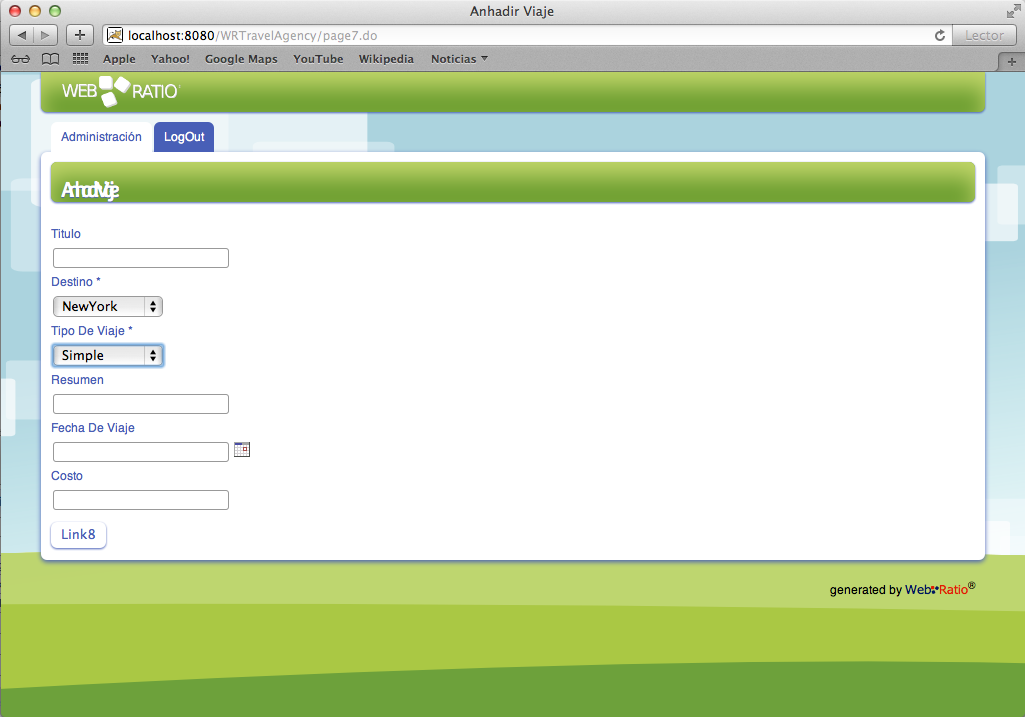
\includegraphics[width=1.0\textwidth]{figure/fig_WRTA_Administracion.png}
				\newline
				\textbf{Fuente:} Elaboraci\'on Propia -- Prototipo en navegador del
				siteview administrativo.
				\label{fig:WRTA_paginaAdministrador}
			\end{figure}
			
			
		\subsection{Siteview Aplicaci\'on}
		\label{ssec:svAplicacion}
			
			El siteview de nombre \textit{Aplicaci\'on} tiene por objetivo el de permitir
			su acceso a diferencia de otros siteviews a $2$ tipos de grupos/usuarios,
			estos son: el \textit{Usuario Registrado en WRTA} y el \textit{Individuo
			Social}, los cuales representan: al usuario que se registr\'o en la
			aplicaci\'on y expondr\'a informaci\'on verdadera o falsa dependiendo aquella
			que brindo al momento del registro, en cambio el segundo representa al
			individuo que se expone no \'unicamente en el aplicativo sino en Internet a
			nivel global.
		
			\begin{figure}[here]
				\centering
				\caption{WRTA: SiteView de acceso restringido para el usuarios e individuos}
				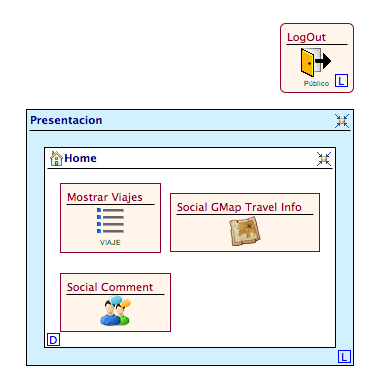
\includegraphics[width=0.5\textwidth]{figure/fig_WRTA_svAplicacion.png}
				\newline
				\textbf{Fuente:} Elaboraci\'on Propia -- Dise\~no del siteview Aplicaci\'on
				\label{fig:WRTA_svAplicacion}
			\end{figure}	
		
			En la Tabla \ref{tab:svAplicacion} se presenta una relaci\'on entre las unidades
			de contenido, el tipo de unidad y la p\'agina a donde
			pertenecen, adem\'as de las unidades de operaci\'on las cuales no pertenecen
			a ninguna p\'agina, en la cual se muestran las unidades suficientes para
			cubrir el requerimiento funcional de mostrar los viajes creados por los
			administradores para su posterior registro en el mismo y como requerimiento
			social el de mostrar al individuo los lugares donde sus amistades se
			encuentran en el mundo, proveyendo as\'i informaci\'on al aplicativo para
			brindarle promociones especificas al individuo, lo cual personaliza m\'as su
			experiencia al individuo en el aplicativo.


			\begin{table}[htbp]
			\centering
			\caption{Unidades utilizadas para SiteView: Aplicaci\'on}
				\begin{tabular}{|l|l|l|}
					\hline
					\textbf{P\'agina}	&	\textbf{Nombre Unidad}	&	\textbf{Tipo Unidad}\\\hline 
					Home				&	Mostrar Viajes			&	Index Unit\\\hline
					Home				&	Social Comment			&	\textit{Social Comment Unit}\\\hline 
					Home				&	Social GMap Travel Info	&	\textit{Social G Maps Unit}\\\hline 
					\multicolumn{1}{|c|}{---}&	LogOut				&	Logout Unit	\\\hline
				\end{tabular}
			\newline
			Fuente: Elaboraci\'on propia -- Resumen de unidades de contenido y de
			operaci\'on para SiteView: Aplicaci\'on.
			\label{tab:svAplicacion}
			\end{table}
 
			En la Figura \ref{fig:WRTA_paginaAplicacion} se puede ver los
			requerimientos funcionales y sociales propios del grupo, usuario e
			individuo social, en el cual se muestra los viajes a los cuales puede
			registrarse, adicional en el componente \textit{Google Maps} se muestra las
			ubicaciones de todos los amigos del individuo social que accedi\'o al
			aplicativo y un bloque de comentarios en el cual el individuo social puede comentar sus
			experiencias y apreciaciones acerca de los viajes realizados con
			anterioridad.

			
			\begin{figure}[here]
				\centering
				\caption{WRTA: Prototipo del siteView propio de la aplicaci\'on}
				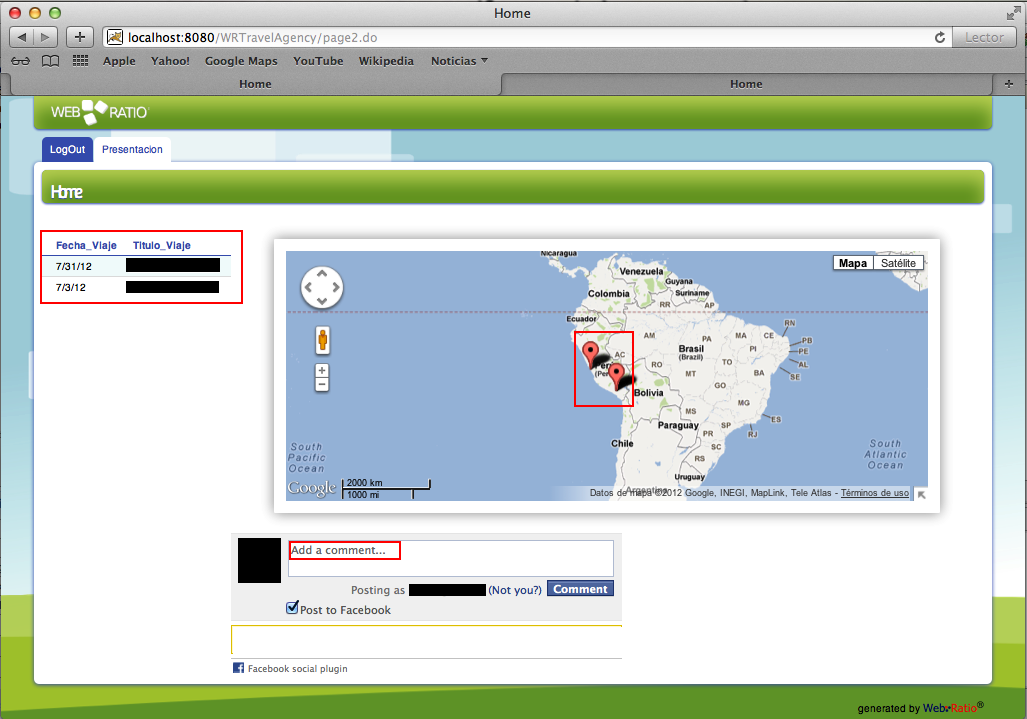
\includegraphics[width=1.0\textwidth]{figure/fig_WRTA_Aplicacion.png}
				\newline
				\textbf{Fuente:} Elaboraci\'on Propia -- Prototipo en navegador del
				siteview del aplicativo.
				\label{fig:WRTA_paginaAplicacion}
			\end{figure}
				
			

		
				
\chapter{CONCLUSIONES} % 1 to 2 pages
\label{chap:Conclusions}

\begin{itemize}
  \item Los seres humanos son seres sociales por naturaleza, por consiguiente
  todo aquello que hacen, incluso el software que desarrollan y usan, debe de
  ser tambi\'en social.

  \item Los pilares de la Web Social son:
  \begin{itemize}
  	\item Comunicaci\'on (multi--direccional)
  	\item Interacci\'on
	\item Cooperaci\'on
  	\item Contribuci\'on
  	\item Individualidad
  	\item Representatividad o diferenciaci\'on
  \end{itemize}  
  %Las 4 tablas de la bd bindan estas caracteristicas a nivel de bd
  \item La inteligencia colectiva es el recurso m\'as importante a ser
  explotado.
  \item La Web Social busca eliminar la relaci\'on actualmente existente entre
  usuario final y desarrollador, convirtiendo al usuario final como parte del
  ciclo de vida del software, convirti\'endolo en parte desarrollador y parte
  tester.
  \item La forma m\'as confiable de conocer la naturaleza de un producto es
  mediante los \textbf{comentarios} de otros individuos que hayan tenido
  contacto con el mismo.
  \item Con la Web Social el marketing ad--hoc es posible.
  \item A nivel de base de datos se observa que las tablas relacionadas a
  requerimientos funcionales estar\'an enlazadas a las tablas nativas de
  \ac{WebML} y aquellas tablas relacionadas a requerimientos sociales estar\'an
  enlazadas a las tablas nativas de Social WebML.
\end{itemize}




\renewcommand{\chapternamenum}{\scshape---~Anexo~}
\appendix
\clearpage




\chapter{MODELADO DE CUSTOM UNITS\\De Andreis -- \cite{Andreis2010}}
\label{ane:customUnits}
	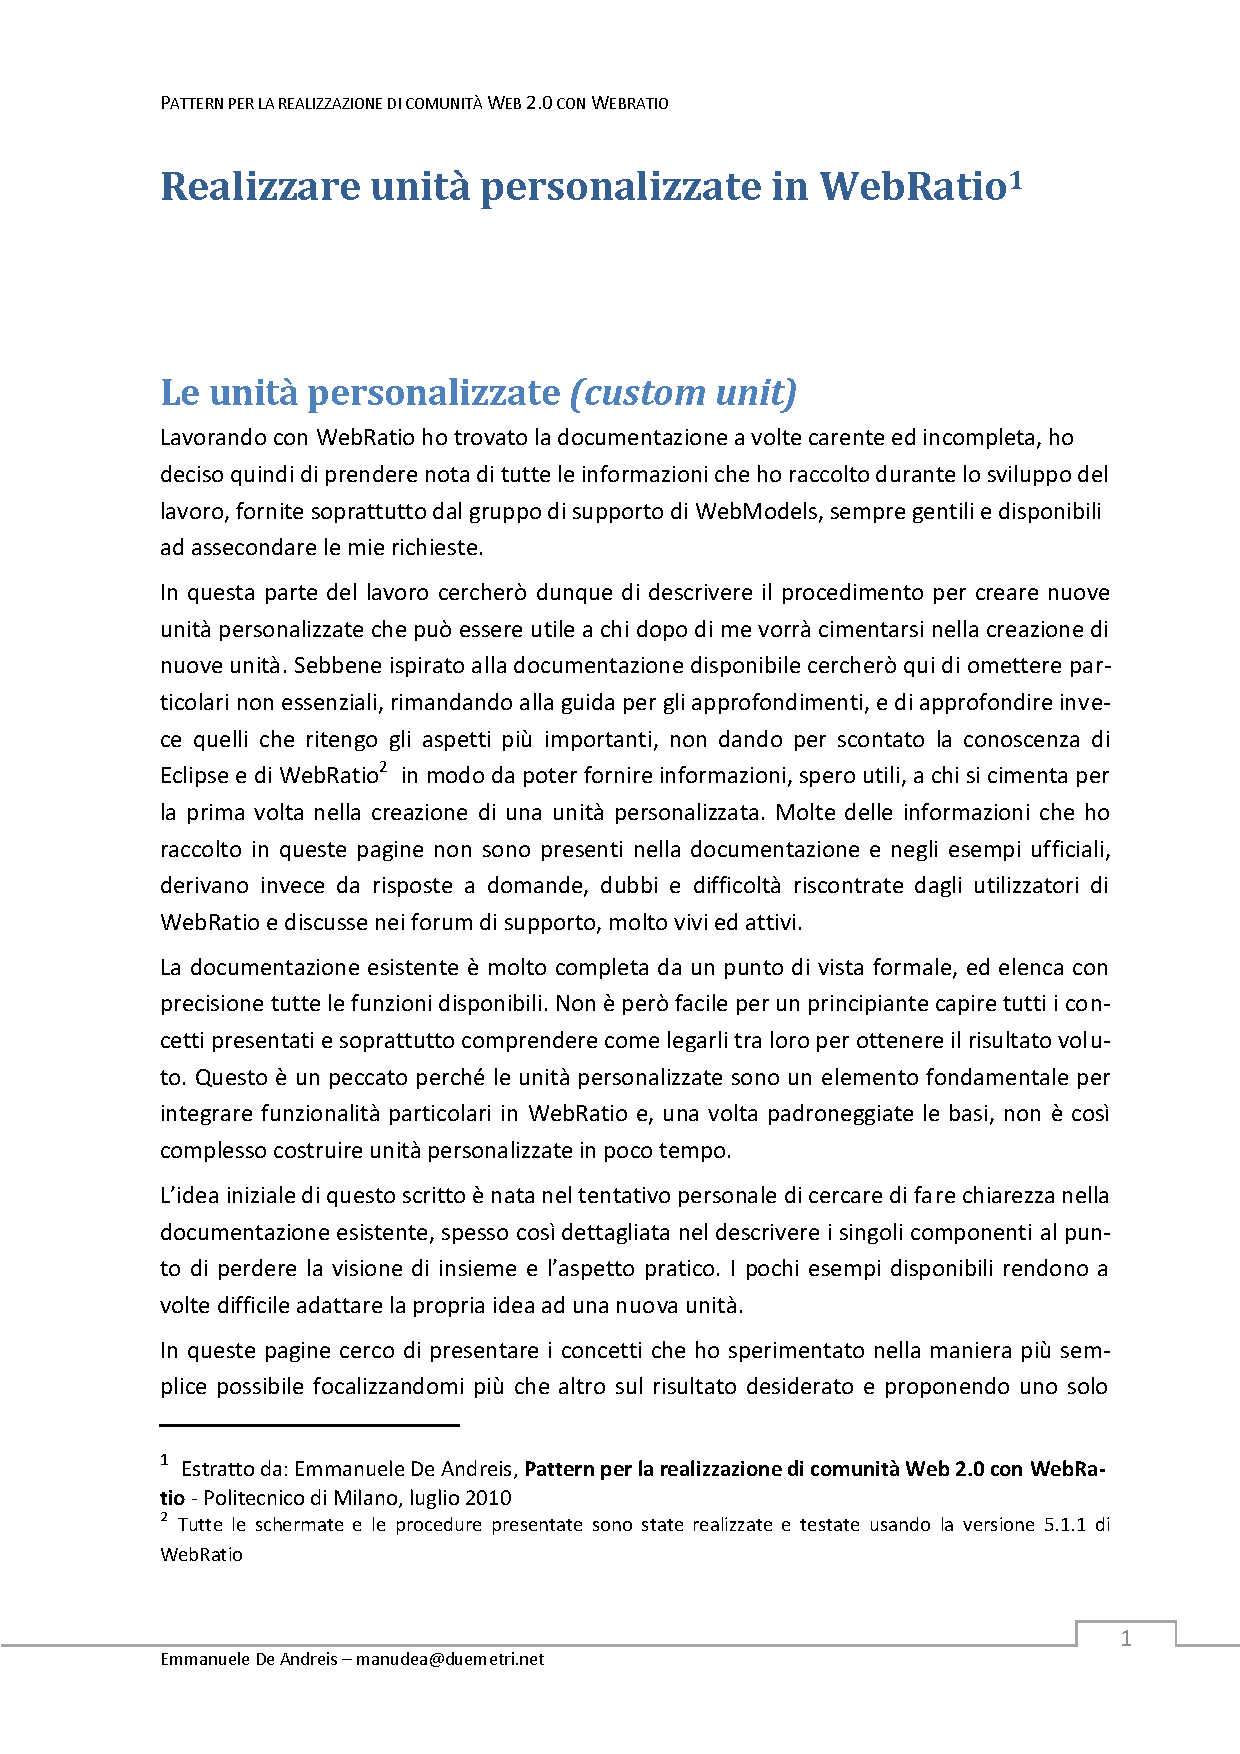
\includepdf[pages={1-22}]{include/anexo_customUnits}



\chapter{CODIFICACI\'ON DE CUSTOM UNITS}
\label{ane:srcCustomUnits}
\section{SocialLoginUnitService}
\begin{landscape}
\begin{lstlisting}[language=java, style=eclipse]  
package com.webratio.units.custom.socialloginunit;
import java.util.Map;

//Bibliotecas usadas para la integraci\'on con WebRatio
import org.dom4j.Element;
import com.webratio.rtx.RTXConstants;
import com.webratio.rtx.RTXContentUnitService;
import com.webratio.rtx.RTXException;
import com.webratio.rtx.RTXManager;
import com.webratio.rtx.RTXOperationUnitService;
import com.webratio.rtx.beans.ExtendedOperationUnitBean;
import com.webratio.rtx.core.AbstractService;
import com.webratio.rtx.core.BeanHelper;
import com.webratio.rtx.core.DescriptorHelper;


public class SocialLoginUnitService extends AbstractService implements RTXContentUnitService, RTXOperationUnitService{
	String myResult="";
	String app_id="";
	
	public SocialLoginUnitService(String id, RTXManager mgr, Element descr) {
		super(id, mgr, descr);
		
		//Seleccionado el elemento que contiene el valor de la unidad actual
		Element currentUnit = descr.element("SocialLoginUnit");
		
		//Lectura de parametros estaticos
		try{
			app_id = DescriptorHelper.getAttribute(currentUnit, "app_id", true, this).toString();
		}
		catch(Exception e){}
	}
	

    public Object computeParameterValue(String outputParamName, Map pageContext, Map sessionContext) throws RTXException {
		SocialLoginUnitBean unitBean = getUnitBean(pageContext, sessionContext);
		return BeanHelper.getBeanProperty(unitBean, outputParamName,
				this);
    }

    public Object execute(Map localContext, Map sessionContext) throws RTXException {
    	SocialLoginUnitBean unitBean = (SocialLoginUnitBean)getUnitBean(localContext, sessionContext);
		if (unitBean == null) {
			return null;
		}
		return unitBean;
    }

    public void dispose() {
        // TODO Auto-generated method stub
    } 

	protected SocialLoginUnitBean getUnitBean(Map pageContext, Map sessionContext)
	throws RTXException {
		SocialLoginUnitBean unitBean = (SocialLoginUnitBean) pageContext
		.get('_' + getId());
		if (unitBean == null ||
				Boolean.TRUE.equals(pageContext.get(RTXConstants.IN_OPERATION_KEY)))
		{
			unitBean = (SocialLoginUnitBean) createUnitBean(pageContext, sessionContext);
		}
		
		unitBean.put("uid", app_id);
		
		pageContext.put('_' + getId(), unitBean);
		return unitBean;
	}
	 
	private ExtendedOperationUnitBean createUnitBean(Map pageContext,
			Map sessionContext)throws RTXException {
		
		SocialLoginUnitBean bean =  new SocialLoginUnitBean();

		myResult = "Hello World!!";
		try {
			bean.put("myResult", myResult);
			bean.put("uid", 1);
			
			bean.setResultCode(RTXConstants.SUCCESS_CODE);

		} catch (Exception e) {
			logError("Error in executing http method", e);
			bean.setResultCode(RTXConstants.ERROR_CODE);
		}
		return bean;
	}
}   
\end{lstlisting}
\end{landscape}





\section{GetSocialDataUnitService}
\begin{landscape}
\begin{lstlisting}[language=java, style=eclipse] 
package com.webratio.units.custom.getsocialdataunit;
import java.util.Map;
//Biblioteca para poder extraer la sesi\'on como un objeto y poder trabajar con este
import javax.servlet.http.HttpServletRequest;

//Biblioteca para poder desencriptar los parametros traids desde la parte cliente
import org.apache.commons.codec.binary.Base64;

//Bibliotecas usadas para la integraci\'on con WebRatio
import org.dom4j.Element;
import com.webratio.rtx.RTXConstants;
import com.webratio.rtx.RTXContentUnitService;
import com.webratio.rtx.RTXException;
import com.webratio.rtx.RTXManager;
import com.webratio.rtx.core.AbstractService;
import com.webratio.rtx.core.BeanHelper;


public class GetSocialDataUnitService extends AbstractService implements RTXContentUnitService{
	private String uid_social_network;
	private String name_social_network;

	public GetSocialDataUnitService(String id, RTXManager mgr, Element descr) throws RTXException {
		super(id, mgr, descr);
	}

	public Object computeParameterValue(String outputParamName, Map pageContext, Map sessionContext) throws RTXException {
		//Para enviar los parametros de sesi\'on para el link de output
		GetSocialDataUnitBean unitBean = getUnitBean(pageContext, sessionContext);
		return BeanHelper.getBeanProperty(unitBean, outputParamName,
				this);
	}

	public Object execute(Map pageContext, Map sessionContext) throws RTXException {
		GetSocialDataUnitBean unitBean = getUnitBean(pageContext, sessionContext);
		if (unitBean == null) {
			return null;
		}
		return unitBean;
	}

	public void dispose() {
		// TODO Auto-generated method stub
	}

	@SuppressWarnings("unchecked")
	protected GetSocialDataUnitBean getUnitBean(Map pageContext, Map sessionContext)
	throws RTXException {
		//Extracci\'on de la sesi\'on
		HttpServletRequest request = (HttpServletRequest) pageContext.get(RTXConstants.HTTP_SERVLET_REQUEST_KEY);
		
		//Extracci\'on de parametros de la sesi\'on y encriptaci\'on
		uid_social_network = request.getParameter( "slu_uid" );
		name_social_network = request.getParameter( "slu_n" );
		try{
			uid_social_network = new String(Base64.decodeBase64(uid_social_network));
			name_social_network = new String(Base64.decodeBase64(name_social_network));
		}catch(Exception e){}	

		GetSocialDataUnitBean unitBean = (GetSocialDataUnitBean) pageContext.get('_' + getId());
		if (unitBean == null) {
			unitBean = new GetSocialDataUnitBean();

			//Inserci\'on de datos a la sesi\'on
			try {
				unitBean.put("name", name_social_network);
				unitBean.put("uid", uid_social_network);
				unitBean.setResultCode(RTXConstants.SUCCESS_CODE);

			} catch (Exception e) {
				logError("Error in executing http method", e);
				unitBean.setResultCode(RTXConstants.ERROR_CODE);
			}


		}
		pageContext.put('_' + getId(), unitBean);

		return unitBean;
	}
}

\end{lstlisting}
\end{landscape}


\section{SocialCommentUnitService}
\begin{landscape}
\begin{lstlisting}[language=java, style=eclipse] 
package com.webratio.units.custom.socialcommentunit;
import java.util.Map;
import org.dom4j.Element;
import com.webratio.rtx.RTXContentUnitService;
import com.webratio.rtx.RTXException;
import com.webratio.rtx.RTXManager;
import com.webratio.rtx.core.AbstractService;


public class SocialCommentUnitService extends AbstractService implements RTXContentUnitService{

    public SocialCommentUnitService(String id, RTXManager mgr, Element descr) throws RTXException {
        super(id, mgr, descr);
        // TODO Auto-generated constructor stub
    }

    public Object computeParameterValue(String outputParamName, Map pageContext, Map sessionContext) throws RTXException {
        // TODO Auto-generated method stub
        return null;
    }

    public Object execute(Map pageContext, Map sessionContext) throws RTXException {
        // TODO Auto-generated method stub
        return null;
    }

    public void dispose() {
        // TODO Auto-generated method stub
    }

}
\end{lstlisting}
\end{landscape}



\section{SocialGMapsUnitService}
\begin{landscape}
\begin{lstlisting}[language=java, style=eclipse] 
package com.webratio.units.custom.socialgmapsunit;
import java.util.Map;
import org.dom4j.Element;
import com.webratio.rtx.RTXContentUnitService;
import com.webratio.rtx.RTXException;
import com.webratio.rtx.RTXManager;
import com.webratio.rtx.core.AbstractService;


public class SocialGMapsUnitService extends AbstractService implements RTXContentUnitService{

    public SocialGMapsUnitService(String id, RTXManager mgr, Element descr) throws RTXException {
        super(id, mgr, descr);
        // TODO Auto-generated constructor stub
    }

    public Object computeParameterValue(String outputParamName, Map pageContext, Map sessionContext) throws RTXException {
        // TODO Auto-generated method stub
        return null;
    }

    public Object execute(Map pageContext, Map sessionContext) throws RTXException {
        // TODO Auto-generated method stub
        return null;
    }

    public void dispose() {
        // TODO Auto-generated method stub
    }

}
\end{lstlisting}
\end{landscape}
\backmatter
\pagestyle{plain} 

% Bibliography
%\bibliographystyle{authordate4}% se comento en preamble.tex los newcomand de
% reference
\bibliographystyle{ieeetr}
\bibliography{main2}




\end{document}
